\chapter{Preliminaries}\label{ch:preliminaries}
\vspace*{-6mm}
\chapterquote{The present d-separates the future from the past.}{Stefano Ermon}

In this chapter, we provide background on concepts used in this thesis: sequential decision making frameworks, planning algorithms, surrogate modeling, and safety~validation.

\section{Markov Decision Processes}
The \textit{Markov decision process} (MDP) \cite{bellman1957dynamic,dmbook}, shown in \cref{fig:mdp_ddn}, is a sequential decision making framework used to model problems where the state-transition dynamics are uncertain.
An MDP is defined by the tuple $\langle \mathcal{S}, \mathcal{A}, T, R, \gamma \rangle$, where $\mathcal{S}$ is the space of all states $s \in \mathcal{S}$ (discrete or continuous), the action space is denoted $\mathcal{A}$ where $a \in \mathcal{A}$ (discrete or continuous), the state-transition function is denoted $s' \sim T(\cdot \mid s, a)$ for a next state $s'$, the reward function is denoted $r = R(s,a)$ or $r = R(s,a,s')$, and the discount factor $\gamma \in [0, 1)$ controls the problem's degree of myopia, where the discount factor could be $\gamma = 1$ for undiscounted problems (noting that the focus of this thesis is on \textit{discounted MDPs}).

To solve an MDP, planning algorithms (\cref{sec:planning_algs}) construct a policy $\pi$ that maps states to actions: $a = \pi(s)$ or $a \sim \pi(\cdot \mid s)$.
The objective of planning algorithms is to find a policy that maximizes the expected discounted sum of rewards (referred to as the \textit{value}):
\begin{equation}
    \operatornamewithlimits{maximize}_\pi \,\, V^\pi(s_0) = \mathbb{E}_\pi \Bigg[ \sum_{t=0}^\infty \gamma^t R(s_t, a_t) \mid s_0 \sim \mathcal{S}_0,\, a_t \sim \pi(\cdot \mid s_t) \Bigg]
\end{equation}
where the initial state $s_0$ is sampled from the initial state distribution $\mathcal{S}_0$ (also denoted $\mu_0$).

\begin{figure}[t]
    \centering
    \begin{subfigure}[t]{0.49\linewidth}
        \centering
        \tikzset{
    >=stealth',
    every node/.style={line width=1pt},
    every path/.append style={line width=1pt},
}
\begin{tikzpicture}[x=1cm, y=1cm, baseline=(current bounding box.north)]
    \node[minimum size=1cm, draw=pastelBlue!60!black, fill=pastelBlue!10, circle] (s) {$s_t$};
    \node[minimum size=1cm, draw=black, fill=white, circle, right=1cm of s] (s2) {$s_{t+1}$};
    \node[minimum size=1.3cm, draw=black, fill=white, diamond, above=0.5cm of s] (r) {$r_t$};
    \node[minimum size=1cm, draw=black, fill=white, rectangle, above=0.5cm of r] (a) {$a_t$};
    \node[minimum size=1cm, draw=black, fill=white, rectangle, left=1cm of a] (am1) {$a_{t-1}$};

    \node[minimum size=1.3cm, draw=lightgray, fill=white, diamond] (rm1) at (am1|-r) {\textcolor{lightgray}{$r_{t-1}$}};
    \node[minimum size=1cm,   draw=lightgray, fill=white, circle]  (sm1) at (am1|-s) {\textcolor{lightgray}{$s_{t-1}$}};

    \node[minimum size=1cm,   draw=lightgray, fill=white, rectangle] (ap1) at (s2|-a) {\textcolor{lightgray}{$a_{t+1}$}};
    \node[minimum size=1.3cm, draw=lightgray, fill=white, diamond]   (rp1) at (s2|-r) {\textcolor{lightgray}{$r_{t+1}$}};

    \draw[->] (s) -- (s2);
    \draw[->] (s) -- (r);
    \draw[->] (a) -- (r);
    \draw[->] (a) [out=0, in=145, looseness=0.8] to (s2);
    \draw[->] (am1) [out=0, in=145, looseness=0.8] to (s);
\end{tikzpicture}

        \vspace*{15mm}
        \caption{The MDP problem formulation.}\label{fig:mdp_ddn}
    \end{subfigure}
    \hfill
    \begin{subfigure}[t]{0.49\linewidth}
        \centering
        \tikzset{
    >=stealth',
    every node/.style={line width=1pt},
    every path/.append style={line width=1pt},
}
\begin{tikzpicture}[x=1cm, y=1cm, baseline=(current bounding box.north)]
    \node[minimum size=1cm, draw=black, fill=lightgray!30, circle] (s) {$s_t$};
    \node[minimum size=1cm, draw=black, fill=lightgray!30, circle, right=1cm of s] (s2) {$s_{t+1}$};
    \node[minimum size=1cm, draw=pastelBlue!60!black, fill=pastelBlue!10, circle, below=0.5cm of s] (o) {$o_t$};
    \node[minimum size=1.3cm, draw=black, fill=white, diamond, above=0.5cm of s] (r) {$r_t$};
    \node[minimum size=1cm, draw=black, fill=white, rectangle, above=0.5cm of r] (a) {$a_t$};
    \node[minimum size=1cm, draw=black, fill=white, rectangle, left=1cm of a] (am1) {$a_{t-1}$};

    \node[minimum size=1.3cm, draw=lightgray, fill=white, diamond] (rm1) at (am1|-r) {\textcolor{lightgray}{$r_{t-1}$}};
    \node[minimum size=1cm,   draw=lightgray, fill=lightgray!30, circle]  (sm1) at (am1|-s) {\textcolor{lightgray}{$s_{t-1}$}};
    \node[minimum size=1cm,   draw=lightgray, fill=white, circle]  (om1) at (am1|-o) {\textcolor{lightgray}{$o_{t-1}$}};

    \node[minimum size=1cm,   draw=lightgray, fill=white, rectangle] (ap1) at (s2|-a) {\textcolor{lightgray}{$a_{t+1}$}};
    \node[minimum size=1.3cm, draw=lightgray, fill=white, diamond]   (rp1) at (s2|-r) {\textcolor{lightgray}{$r_{t+1}$}};
    \node[minimum size=1cm,   draw=lightgray, fill=white, circle]    (op1) at (s2|-o) {\textcolor{lightgray}{$o_{t+1}$}};

    \draw[->] (s) -- (o);
    \draw[->] (s) -- (s2);
    \draw[->] (s) -- (r);
    \draw[->] (a) -- (r);
    \draw[->] (a) [out=0, in=145, looseness=0.8] to (s2);
    \draw[->] (am1) [out=0, in=145, looseness=0.8] to (s);
\end{tikzpicture}

        \caption{The POMDP problem formulation.}\label{fig:pomdp_ddn}
    \end{subfigure}
    \caption{Dynamic decision networks for the MDP and POMDP problem formulations.}
    \label{fig:dnns}
\end{figure}

\section{Partially Observable Markov Decision Processes}\label{sec:pomdps}

The \textit{partially observable Markov decision process} (POMDP) \cite{cassandra1998exact,kaelbling1998planning,dmbook} is a model for sequential decision making problems where the true state is unobservable, modeling the real world.
Defined by the tuple $\langle \mathcal{S}, \mathcal{A}, \mathcal{O}, T, R, O, \gamma \rangle$, 
the POMDP is an extension to the MDP framework used in reinforcement learning and planning with the addition of an observation space $\mathcal{O}$ (where $o \in \mathcal{O}$) and observation model $O(o \mid a, s')$.
Given a current state $s \in \mathcal{S}$ and taking an action $a \in \mathcal{A}$, the agent transitions to a new state $s'$ using the transition model $s' \sim T(\cdot \mid s, a)$.
Without access to the true state, an observation is received $o \sim O(\cdot \mid a, s')$ and used to update the belief $b$ over the possible next states $s'$ to get the posterior:
\begin{equation}    
    b'(s') \propto O(o \mid a, s')\int T(s' \mid s, a)b(s) \diff s
\end{equation}
where the belief is a distribution over states---capturing state uncertainty.
Examples of the different types of belief representations and updating methods are detailed in \cref{sec:belief_updating}.

A stochastic POMDP policy $\pi(a \mid b)$ is defined as the distribution over actions given the current belief $b$.
After taking an action $a \sim \pi(\cdot \mid b)$, the agent receives a reward $r$ from the environment according to the reward function $R: \mathcal{S} \times \mathcal{A} \to \mathbb{R}$ or $R: \mathcal{S} \times \mathcal{A} \times \mathcal{S} \to \mathbb{R}$ using the next state.
Note that the policy may be deterministic, i.e., $a = \pi(b)$.

\subsection{Belief-State MDPs}\label{sec:belief_state_mdps}
In \textit{belief-state MDPs}, a POMDP is converted to an MDP by treating the belief as a state \cite{kaelbling1998planning,dmbook}.
The reward function then becomes a weighting of the state-based reward function:
\begin{align}\label{eq:belief_reward}
    R_b(b,a) = \!\int b(s)R(s,a) \,\mathrm{d}s
\end{align}
The belief-state MDP (BMDP) shares the same action space as the underlying POMDP and operates over a belief space $\mathcal{B}$ that is the simplex over the state space $\mathcal{S}$. The belief-state MDP defines a new belief-state transition function $b' \sim T_b(\cdot \mid b, a)$ as:
\begin{align}
    s \sim b(\cdot) \qquad s' \sim T(\cdot \mid s, a) \qquad o \sim O(\cdot \mid a, s') \qquad b' \leftarrow \textsc{Update}(b, a, o) \label{eq:tb_update}
\end{align}
where the belief update can be done using methods from \cref{sec:belief_updating}.
Therefore, the belief-state MDP is defined by the tuple $\langle \mathcal{B}, \mathcal{A}, T_b, R_b, \gamma \rangle$ with the finite-horizon discount factor $\gamma \in [0,1)$ that controls the effect that future rewards have on the current action.

The objective to solve BMDPs is to find a policy $\pi$ that maximizes the \textit{value function}:
\begin{equation}
    \operatornamewithlimits{maximize}_\pi \,\, V^\pi(b_0) = \mathbb{E}_\pi \left[\sum_{t=0}^T \gamma^t R_b(b_t,a_t) \bigmid\mid b_t \sim T_b(\cdot \mid s_t, a_t),\, a_t \sim \pi(\cdot \mid b_t) \right]
\end{equation}
given an initial belief $b_0$, the transitioned belief $b_t$, and an action $a_t$ from the policy $\pi$.
Different belief updating methods are used depending on the problem structure (i.e., discrete or continuous state and observation spaces and potentially nonlinear transition dynamics).

\subsection{Belief Updating}\label{sec:belief_updating}
Beliefs can be represented in different ways, namely parametric or non-parametric representations \cite{dmbook}.
For parametric beliefs, the belief distribution is represented by a set of parameters for a fixed distribution family (e.g., categorical distribution where probability mass is assigned to each discrete state or multivariate Gaussian distributions for continuous problems).
For non-parametric beliefs, the belief distribution is represented by a collection of states (often called \textit{state particles}), which are points sampled from the posterior state space.
Depending on the belief representation, different belief updating algorithms can be used.

\paragraph{Discrete state filtering.}
If the state and observation spaces are discrete, then we can perform exact belief updates \cite{dmbook}.
This means we can arrive at an analytical solution to the belief updating without approximations.
For discrete states and observations with relatively small space sizes $|\mathcal{S}|$ and $|\mathcal{O}|$, we can use the \textit{discrete state filter} (also called \textit{recursive Bayesian estimation}) to infer the unknown belief distribution.
The discrete state filter updates the belief recursively over time, using the Markov assumption which says that the current state $s_t$ is conditionally independent of all past states and actions given the previous state $s_{t-1}$ and action $a_{t-1}$.
Due to the independence assumption, if an agent with belief $b$ takes an action $a$ and receives an observation $o$, then the new belief $b^\prime$ becomes:
\begin{align*}
    b^\prime(s^\prime) &= P(s^\prime \mid b, a, o)\\
                       &\propto P(o \mid b, a, s^\prime) P(s^\prime \mid b, a) \tag{Bayes' rule}\\
                       &\propto O(o \mid a, s^\prime) P(s^\prime \mid b, a)\tag{observation definition}\\
                       &\propto O(o \mid a, s^\prime) \sum_s P(s^\prime \mid b, a, s) P(s \mid b, a) \tag{law of total probability}\\
                       &\propto O(o \mid a, s^\prime)\sum_s T(s^\prime \mid s, a)b(s) \tag{state transition model}
\end{align*}
We can call this the \textit{unnormalized} belief $\hat{b}'$. The exact belief update is then normalized so that beliefs sum to one:
\begin{equation}
    b^\prime(s^\prime) = \frac{\hat{b}'(s')}{\sum_{s^{\prime\prime}} \hat{b}'(s^{\prime\prime})} = \frac{O(o \mid a, s^\prime)\sum_s T(s^\prime \mid s, a)b(s)}{\sum_{s^{\prime\prime}} O(o \mid a, s^{\prime\prime}) \sum_s T(s^{\prime\prime} \mid s, a) b(s)}
\end{equation}
This ensures that $b'(s') \ge 0$ for all $s' \in \mathcal{S}$ and that $\sum_{s'} b'(s') = 1$, making $b'$ a valid probability distribution (i.e, a valid probability mass function in the discrete case).

\paragraph{Kalman filtering.}
So far, we have shown how to update beliefs for discrete POMDPs (discrete states and observations).
In continuous state and observation problems, updating the belief involves integrating instead of summing:
\begin{equation}
    b'(s') \propto O(o \mid a, s')\int T(s' \mid s, a)b(s) \diff s
\end{equation}
Integrating over the state space may be intractable; therefore, methods have been developed to address this challenge.
If certain linear-Gaussian assumptions are met, then we can update the belief using a \textit{Kalman filter} \cite{kalman1960new,welch1995introduction,dmbook}.
In a standard Kalman filter, we can compute the exact belief update under the following assumptions.
We assume the transition model $T$ and observation model $O$ to be linear-Gaussian and assume the belief $b$ to be Gaussian, then:
\begin{align*}
    T(\mathbf{s}^\prime \mid \mathbf s, \mathbf a) &= \mathcal{N}(\mathbf{s}^\prime \mid \mathbf{T}_s \mathbf{s} + \mathbf{T}_a \mathbf{a},\, \mat{\Sigma}_s) \tag{linear-Gaussian transition} \\
    O(\mathbf o \mid \mathbf{s}^\prime) &= \mathcal{N}(\mathbf o \mid \mathbf{O}_s \mathbf{s}^\prime,\, \mat{\Sigma}_o) \tag{linear-Gaussian observation} \\
    b(\mathbf{s}) &= \mathcal{N}(\mathbf{s} \mid \vec{\mu}_b,\, \mat{\Sigma}_b) \tag{Gaussian belief}
\end{align*}
where $\vec{\mu}_b$ and $\vec{\Sigma}_b$ are the mean vector and covariance matrix that define the Gaussian belief, the state transition covariance is $\vec{\Sigma}_s$, and the observation covariance is $\vec{\Sigma}_o$.
As shown in \cref{alg:kalman_filter}, the first step is prediction.
The prediction step uses the transition dynamics to get a predicted distribution that is parameterized by the following mean and covariance:
\begin{align}
    \vec{\mu}_p &= \mathbf{T}_s\vec{\mu}_b + \mathbf{T}_a\vec{a} \tag{predicted mean} \\
    \vec{\Sigma}_p &= \mathbf{T}_s\vec{\Sigma}_b\mathbf{T}_s^\top + \vec{\Sigma}_s \tag{predicted covariance}
\end{align}
The update step then uses the prediction to update the belief:
\begin{align}
    \mathbf{K} &= \frac{\vec{\Sigma}_p\mathbf{O}_s^\top}{\mathbf{O}_s\vec{\Sigma}_p\mathbf{O}_s^\top + \vec{\Sigma}_o} \tag{Kalman gain} \\
    \vec{\mu}_b &= \vec{\mu}_p + \mathbf{K}\big(\mathbf{o} - \mathbf{O}_s\vec{\mu}_p\big) \tag{updated mean} \\
    \vec{\Sigma}_b &= \big(\mathbf{I} - \mathbf{K}\mathbf{O}_s \big)\vec{\Sigma}_p \tag{updated covariance}
\end{align}
Here we note that the states, observations, and actions may be vectors $\mathbf{s}$, $\mathbf{o}$, and $\mathbf{a}$, respectively.

\begin{algorithm}[t]
    \caption{Kalman filter belief updater.}
    \label{alg:kalman_filter}
    \begin{algorithmic}
    \Function{KalmanFilter$(b, a, o)$}{}
    \State $(\vec{\mu}_p, \vec{\Sigma}_p) \leftarrow \textproc{KalmanPredict}(b, a)$ \Comment{linear-Gaussian prediction}
    \State $b' \leftarrow \textproc{KalmanUpdate}(b, o, \vec{\mu}_p, \vec{\Sigma}_p)$ \Comment{Gaussian update}
    \State \Return $b'$
    \EndFunction
    \end{algorithmic}
\end{algorithm}


\paragraph{Nonlinear Kalman filtering.}
To address problems with nonlinear dynamics and Gaussian noise, the \textit{extended Kalman filter} (EKF) \cite{julier1997new} was developed. The EKF method requires differentiable functions $\mathbf{f}_T(\mathbf{s}, \mathbf{a})$ and $\mathbf{f}_O(\mathbf{a}, \mathbf{s}')$, where the Gaussian transition function is defined as $T(\mathbf{s}' \mid \mathbf{s}, \mathbf{a}) = \mathcal{N}(\mathbf{s}' \mid \mathbf{f}_T(\mathbf{s}, \mathbf{a}), \vec{\Sigma}_s)$ and the Gaussian observation function is defined as $O(\vec{o} \mid \mathbf{a}, \mathbf{s}') = \mathcal{N}(\mathbf{o} \mid \mathbf{f}_O(\mathbf{a}, \mathbf{s}'), \vec{\Sigma}_o)$ \cite{dmbook}.
The key idea is that the EKF uses a local linear approximation of the nonlinear dynamics.
Another extension to the standard Kalman filter, namely the \textit{unscented Kalman filter} (UKF) \cite{wan2000unscented}, can be applied in cases where the dynamics functions $\mathbf{f}_T$ and $\mathbf{f}_O$ are non-differentiable.
The UKF uses weighted sigma point samples to approximate the continuous Gaussian belief and passes the sigma points through an unscented transform.\footnote{The \textit{unscented transform} was arbitrarily named by Jeffrey Uhlmann, inspired by a colleague's unscented deodorant to prevent the name ``Uhlmann filter'' from sticking (it's derivative-free---how clean!) \cite{unscented2021uhlmann}.}
Sigma points are then updated by the UKF and used to reconstruct the updated $\vec{\mu}_b$ and $\vec{\Sigma}_b$ (instead of updating the nonlinear Gaussian directly).

\paragraph{Particle filtering.}
In problems with large discrete state and observation spaces or continuous problems not well approximated by linear-Gaussian dynamics, other approximations are required to estimate the belief update.
One such method is the \textit{particle filter} \cite{gordon1993novel}, which can represent a broad range of non-parametric distributions \cite{thrun2005probabilistic}.
In a particle filter, the belief is represented as a collection of states where each state in the approximated belief is called a \textit{state particle}.
Shown in \cref{alg:particle_filter}, the particle filter first transitions all state particles through the stochastic transition function $s'_i \sim T(\cdot \mid s_i, a)$ for $s_i \in \mathbf{s}$, where $\mathbf{s}$ is a collection of states approximating the belief, i.e., $b \approx \mathbf{s}$.
The particle filter then weighs each next state based on how likely the input observation $o$ is given the next states $s'_i \in \mathbf{s}'$ and current action $a$.
Then the particles are resampled based on the particle weights, and the new approximated belief (i.e., particle set) is returned.

\begin{algorithm}[h]
    \caption{Particle filter belief updater.}
    \label{alg:particle_filter}
    \begin{algorithmic}
    \Function{ParticleFilter$(\mathbf{s}, a, o)$}{}
    \State $\mathbf{s}^\prime \sim T(\cdot \mid \mathbf{s}, a)$ \Comment{propagate past particles $\mathbf{s}$ through the transition model}
    \State $\mathbf{w} \leftarrow O(o \mid \mathbf{s}^\prime, a)$ \Comment{weight next states based on the observation model}
    \State $\text{particles} \sim \operatorname{SetCategorical}\left(\mathbf{s}^\prime, \frac{\mathbf{w}}{\sum_i w_i}\right)$ \Comment{sample new particles with normalized weights}
    \State \Return $\text{particles}$
    \EndFunction
    \end{algorithmic}
\end{algorithm}


In \cref{ch:ivae}, we learn belief updating surrogates to address problems where the observation likelihood model $O(o \mid a, s')$ may be unknown or hard to compute and where beliefs may not be well approximated directly by Gaussian distributions.

\section{Planning Algorithms}\label{sec:planning_algs}
Separating the \textit{problem structure} (i.e., POMDP definition) from the \textit{solution method} (i.e., planning algorithm) is beneficial as separate research can focus on solution methods given a variety of challenging problems.
This section will outline several different MDP and POMDP solution methods that each have the goal of computing an (approximately) optimal policy $\pi$ that maximizes the expected discounted sum of rewards.

\subsection{Offline Planning}
In \textit{offline planning} algorithms, a policy is constructed offline (i.e., pre-computed) that maps states to actions.
The offline policy can be represented as a lookup table that returns an action for every state.
The offline policy can also be represented as a neural network surrogate, as shown by \textcite{mnih2013playing} in the development of deep Q-learning networks (DQNs).
Although the differences are subtle, this work focuses on \textit{planning algorithms} and not \textit{reinforcement learning algorithms} (such as $Q$-learning \cite{watkins1989learning}).

\paragraph{Planning vs. reinforcement learning.}
In MDP and POMDP \textit{planning}, models of the transitions, rewards, and observations (for POMDPs) are known.
In contrast, in the model-based reinforcement learning (RL) domain (or the partially observable reinforcement learning (PORL) domain), these models are learned along with a policy or value function \cite{sutton2018reinforcement,subramanian2022approximate}.
A key difference between these settings is that RL algorithms reset the agent and learn through experience, while planning algorithms must consider future trajectories from \textit{any state}.
When RL problems have deterministic state transitions, they can be cast as planning problems by replaying the full state trajectory along a path, which may be prohibitively expensive for long-horizon problems.
Both settings are closely related and pose interesting research challenges.
Specifically, sequential planning over given models in high-dimensional, long-horizon POMDPs remains challenging \cite{lauri2022partially}.
The content of this thesis attempts to address some of these challenges.


\subsubsection{Policy Iteration}
In discrete MDPs with relatively small state and action spaces, \textit{policy iteration} \cite{bellman1957dynamic,sutton2018reinforcement} can be used to solve for an optimal policy.
In policy iteration, the optimal policy $\pi^*$ is computed by iterating the following two steps \cite{dmubook}.
Starting with any policy $\pi_0$, policy iteration performs:
\begin{enumerate}
    \item \textbf{Policy evaluation}: Given the current policy, compute the value function.
    \item \textbf{Policy improvement}: Using the value function, compute an improved policy.
\end{enumerate}
During \textit{policy evaluation}, the current policy at iteration $k$ uses dynamic programming to compute the value function for $n$ steps (where $t \in [1,\ldots,n])$:
\begin{equation}
    V^\pi_t(s) = R(s, \pi(s)) + \gamma \sum_{s'} T(s' \mid s, \pi(s)) V^\pi_{t-1}(s') \quad \text{for all } s \in \mathcal{S}
\end{equation}
Then during \textit{policy improvement}, the value function returned from policy evaluation is used to compute the improved policy, again using the Bellman equation:
\begin{equation}
    \pi_{k+1}(s) = \argmax_{a \in \mathcal{A}} \left( R(s,a) + \gamma \sum_{s^\prime} T(s^\prime \mid s, a)V^{\pi_k}(s^\prime) \right)
\end{equation}
The resulting policy is often stored in a lookup table \cite{dmubook} so it can easily be queried during runtime usage (i.e., queries to the pre-computed offline policy online).
In \cref{ch:betazero}, we will use the policy iteration paradigm combined with learning a neural network surrogate of the value function and an action selection policy for high-dimensional POMDPs.


\subsubsection{Value Iteration}\label{sec:value_iteration}
Another offline method to solve for the optimal policy in discrete MDPs is called \textit{value iteration} \cite{bellman1957dynamic}.
Similar to policy iteration, value iteration uses dynamic programming and the Bellman equation to compute the optimal \textit{value} (or \textit{utility}) $V$ iteratively \cite{dmubook}:
\begin{equation}\label{eq:value_function}
    V^*(s) = \max_{a \in \mathcal{A}} \biggl( R(s,a) + \gamma \sum_{s^\prime} T(s^\prime \mid s,a) V^*(s^\prime) \biggr)
\end{equation}
Once the value function has converged, namely $|V_{k-1}(s) - V_k(s)| \le \epsilon$ for all $s \in \mathcal{S}$, the optimal policy $\pi^*$ can then be extracted using the final value function:
\begin{equation}
    \pi^*(s) = \argmax_{a \in \mathcal{A}} \biggl( R(s,a) + \gamma \sum_{s^\prime} T(s^\prime \mid s, a) V^*(s^\prime) \biggr) \label{eq:vi_policy_extraction}
\end{equation}
Similar to policy iteration, the policy output from value iteration can be stored in an efficient lookup table to be queried during online evaluation.


\subsubsection{Local approximation value iteration}
For large or continuous state spaces, approximate dynamic programming can be useful in finding approximately optimal polices for the substructure of the problem \cite{dmubook}.
For a finite set of $n$ discretized states, a function $\beta(s)$ is used to weigh ``nearby'' states, where $\sum_{i=1}^n \beta_i(s) = 1$.
The value $\lambda_i \in \vec{\lambda}$ for each state $s_i$ is used to approximate the value of an arbitrary state as $V(s) = \sum_{i=1}^n \lambda_i \beta_i(s) = \vec{\lambda}^\top \beta(s)$.
Given a discretization of $n$ states, the values are initialized to zero, namely $\vec{\lambda} = \mathbf{0}$, and then the following is iterated until convergence:
\begin{align}
    u_i &= \max_{a \in \mathcal{A}} \left( R(s_i, a) + \gamma \sum_{s' \in s_{1:n}} T(s' \mid s_i, a)\vec{\lambda}^\top \beta(s') \right) \text{ for } i \in [1, \ldots, n] \\
    \vec{\lambda} &= \mathbf{u}
\end{align}
The final policy is extracted the same way as \cref{eq:vi_policy_extraction} except now using the neighboring approximation $\beta(s)$ (also known as a \textit{kernel} function).
To approximately solve POMDPs, \textit{local approximation value iteration} (LAVI), as presented here, can be used by discretizing the belief space and treating the problem as a belief-state MDP---as is done in \cref{ch:betazero}.

\subsection{Online Planning}
In contrast to offline methods, \textit{online planning} algorithms compute the approximately optimal action \textit{during runtime} (i.e., online).
Online methods are often used in problems with large or continuous state, action, and observation spaces.
Instead of explicitly constructing a policy over all states or (discretized) beliefs, online planning algorithms estimate the next best action through a planning procedure, often a best-first tree search.

\subsubsection{Monte Carlo Tree Search (MCTS)}\label{sec:mcts}
Monte Carlo tree search \cite{coulom2007efficient,browne2012survey} is an online, recursive, best-first tree search algorithm to determine the approximately optimal action to take from a given root state of an MDP.
Extensions to MCTS have been applied to POMDPs through several algorithms: \textit{partially observable Monte Carlo planning} (POMCP) treats the state nodes as histories $h$ of action-observation trajectories \cite{silver2010pomcp}, \textit{POMCP with observation widening} (POMCPOW) constructs weighted particle sets at the observation nodes and extends POMCP to fully continuous domains \cite{sunberg2018online}, and \textit{particle filter trees} (PFT) and \textit{information PFT} (IPFT) treat the POMDP as a belief-state MDP and plan directly over the belief-state nodes using a particle filter \cite{sunberg2018online,fischer2020information}.
All variants of MCTS execute the following four steps shown in \cref{fig:background-mcts}.
Because MCTS can be applied to MDPs and belief-state MDPs, this section uses $s$ to represent the state, the history $h$, and the belief state $b$, and will refer to them as ``the state''.


\begin{figure}[t]
    \centering
    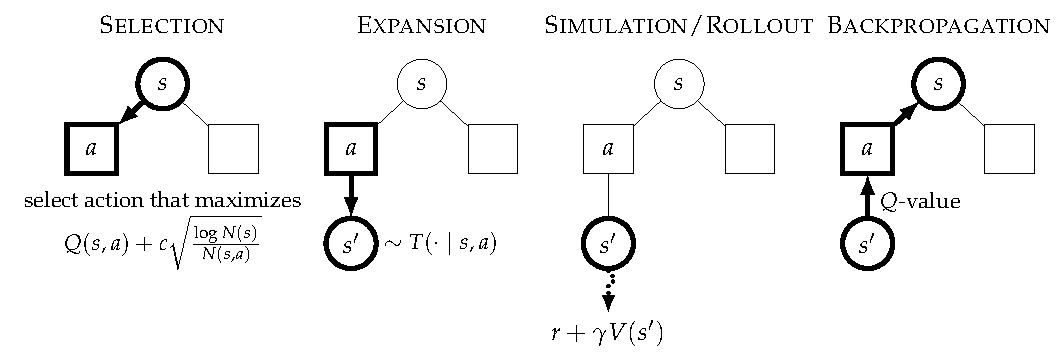
\includegraphics[width=\linewidth]{diagrams/background/mcts.pdf}
    \caption{The four stages of Monte Carlo tree search.}
    \label{fig:background-mcts}
\end{figure}


\begin{enumerate}
    \item \textbf{Selection.}\quad 
    During \textit{selection}, an action is selected from the children of a state node based on criteria that balances exploration and exploitation.
    The \textit{upper-confidence tree} algorithm (UCT) \cite{kocsis2006bandit} is a common criterion that selects an action that maximizes the upper-confidence bound $Q(s, a) + c\sqrt{\log N(s)/N(s,a)}$ 
    where $Q(s,a)$ is the $Q$-value estimate for state-action pair $(s,a)$ with a visit count of $N(s,a)$, the total visit count of $N(s) = \sum_a N(s,a)$ for the children ${a \in A(s)}$, and an exploration constant $c > 0$.
    \textcite{rosin2011multi} introduced the \textit{UCT with predictor} algorithm (PUCT), modified by \textcite{silver2017mastering}, where a predictor $P(s,a)$ guides the exploration towards promising branches and selects an action according to the following:
    \begin{equation}
        \argmax_{a \in A(s)}\ Q(s,a) + c\bigg(P(s,a)\frac{\sqrt{N(s)}}{1 + N(s,a)}\bigg) \label{eq:puct}
    \end{equation}
    
    \item \textbf{Expansion.}\quad 
    In the \textit{expansion} step, the selected action is taken in simulation and the transition model $T(s' \mid s, a)$ is sampled to determine the next state $s'$.
    When the transitions are deterministic, then the child node is always a single state.
    If the transition dynamics are stochastic, techniques to balance the branching factor, such as progressive widening \cite{couetoux2011continuous} and state abstraction refinement \cite{sokota2021monte}, have been proposed.
    
    \item \textbf{Rollout/Simulation.}\quad 
    In the \textit{rollout} step, also called the \textit{simulation} step due to recursively simulating the MCTS tree expansion, the value is estimated through the execution of a rollout policy until termination or using heuristics to approximate the value function from the given state $s'$.
    Expensive rollouts done by AlphaGo \cite{silver2016mastering} were replaced with a value network lookup in AlphaGo Zero and AlphaZero \cite{silver2017mastering,silver2018general}.
    
    \item \textbf{Backpropagation.}\quad 
    Finally, during the \textit{backpropagation} step, the $Q$-value estimate from the rollout is propagated up the path in the tree as a running average.
\end{enumerate}


\paragraph{Root node action selection.}\label{par:root_selection}
After repeating the four steps of MCTS, the final action is selected from the children $a \in A(s)$ of the root state $s$ and executed in the environment.
One way to select the best root node action, referred to as the \textit{robust child} \cite{schadd2009monte, browne2012survey}, selects the action with the highest visit count as $\argmax_a N(s,a)$.
Sampling from the normalized counts, exponentiated by an exploratory temperature $\tau > 0$, is also common \cite{silver2017mastering}.
Another method uses the highest estimated $Q$-value as $\argmax_a Q(s,a)$.
Both criteria have been shown to have problem-based trade-offs \cite{browne2012survey}.


\paragraph{Double progressive widening.}\label{sec:dpw}
To handle stochastic state transitions and large or continuous state and action spaces, double progressive widening (DPW) balances between sampling new nodes to expand or selecting from existing nodes already in the tree \cite{couetoux2011continuous}.
Two hyperparameters $\alpha \in [0,1]$ and $k \ge 0$ control the branching factor.
If the number of actions tried from state $s$ is less than $kN(s)^\alpha$, then a new action is sampled from the action space and added as a child of node $s$.
Likewise, if the number of expanded states from node $(s,a)$ is less than $kN(s,a)^\alpha$, then a new state is sampled from the transition function $s' \sim T(\cdot \mid s, a)$ and added as a child.
If the state widening condition is not met, then a next state is sampled from the existing children.
Typically, different parameters $(\alpha_a, k_a)$ and $(\alpha_s, k_s)$ are used.

\section{Surrogate Modeling}
A \textit{surrogate model} is an approximate function that acts as a ``stand-in'' for unknown, complex, or more expensive functions or simulators \cite{forrester2008engineering}.
Concretely, a surrogate model is a function $\hat{f}(\mathbf{x})$ that approximates a true function $f(\mathbf{x})$ for some input domain $\mathbf{x} \in \mathcal{X}$.
Two commonly used surrogate models studied in this work are Gaussian processes (probabilistic surrogate models) \cite{williams2006gaussian} and neural networks (which can handle high-dimensional data) \cite{hornik1989multilayer}.

\subsection{Gaussian Processes as Probabilistic Surrogate Models}\label{sec:gp}
Probabilistic surrogate models are particularly useful in Bayesian optimization when we want to maximize or minimize some expensive, black-box function $f(\mathbf{x})$.


\begin{figure}[b!]
    \centering
    \resizebox{0.85\textwidth}{!}{%
        % Recommended preamble:
% \usetikzlibrary{arrows.meta}
% \usetikzlibrary{backgrounds}
% \usepgfplotslibrary{patchplots}
% \usepgfplotslibrary{fillbetween}
% \pgfplotsset{%
%     layers/standard/.define layer set={%
%         background,axis background,axis grid,axis ticks,axis lines,axis tick labels,pre main,main,axis descriptions,axis foreground%
%     }{
%         grid style={/pgfplots/on layer=axis grid},%
%         tick style={/pgfplots/on layer=axis ticks},%
%         axis line style={/pgfplots/on layer=axis lines},%
%         label style={/pgfplots/on layer=axis descriptions},%
%         legend style={/pgfplots/on layer=axis descriptions},%
%         title style={/pgfplots/on layer=axis descriptions},%
%         colorbar style={/pgfplots/on layer=axis descriptions},%
%         ticklabel style={/pgfplots/on layer=axis tick labels},%
%         axis background@ style={/pgfplots/on layer=axis background},%
%         3d box foreground style={/pgfplots/on layer=axis foreground},%
%     },
% }

\begin{tikzpicture}[/tikz/background rectangle/.style={fill={rgb,1:red,1.0;green,1.0;blue,1.0}, draw opacity={1.0}}, show background rectangle]
\begin{axis}[point meta max={nan}, point meta min={nan}, legend cell align={left}, legend columns={2}, title={}, title style={at={{(0.5,1)}}, anchor={south}, font={{\fontsize{20.0 pt}{26.0 pt}\selectfont}}, color={rgb,1:red,0.0;green,0.0;blue,0.0}, draw opacity={1.0}, rotate={0.0}}, legend style={color={rgb,1:red,0.0;green,0.0;blue,0.0}, draw opacity={1.0}, line width={0.5}, solid, fill={rgb,1:red,1.0;green,1.0;blue,1.0}, fill opacity={1.0}, text opacity={1.0}, font={{\fontsize{9.0 pt}{11.700000000000001 pt}\selectfont}}, text={rgb,1:red,0.0;green,0.0;blue,0.0}, cells={anchor={center}}, at={(0.02, 0.98)}, anchor={north west}}, axis background/.style={fill={rgb,1:red,1.0;green,1.0;blue,1.0}, opacity={1.0}}, anchor={north west}, xshift={1.0mm}, yshift={-1.0mm}, width={150.4mm}, height={51.5mm}, scaled x ticks={false}, xlabel={}, x tick style={color={rgb,1:red,0.0;green,0.0;blue,0.0}, opacity={1.0}}, x tick label style={color={rgb,1:red,0.0;green,0.0;blue,0.0}, opacity={1.0}, rotate={0}}, xlabel style={at={(ticklabel cs:0.5)}, anchor=near ticklabel, at={{(ticklabel cs:0.5)}}, anchor={near ticklabel}, font={{\fontsize{10.5 pt}{13.65 pt}\selectfont}}, color={rgb,1:red,0.0;green,0.0;blue,0.0}, draw opacity={1.0}, rotate={0.0}}, xmajorgrids={true}, xmin={-10.049999999999999}, xmax={10.049999999999999}, xticklabels={{$-10$,$-5$,$0$,$5$,$10$}}, xtick={{-10.0,-5.0,0.0,5.0,10.0}}, xtick align={inside}, xticklabel style={font={{\fontsize{10.5 pt}{13.65 pt}\selectfont}}, color={rgb,1:red,0.0;green,0.0;blue,0.0}, draw opacity={1.0}, rotate={0.0}}, x grid style={color={rgb,1:red,0.0;green,0.0;blue,0.0}, draw opacity={0.1}, line width={0.25}, solid}, x axis line style={color={rgb,1:red,0.0;green,0.0;blue,0.0}, draw opacity={1.0}, line width={0.5}, solid}, scaled y ticks={false}, ylabel={}, y tick style={color={rgb,1:red,0.0;green,0.0;blue,0.0}, opacity={1.0}}, y tick label style={color={rgb,1:red,0.0;green,0.0;blue,0.0}, opacity={1.0}, rotate={0}}, ylabel style={at={(ticklabel cs:0.5)}, anchor=near ticklabel, at={{(ticklabel cs:0.5)}}, anchor={near ticklabel}, font={{\fontsize{10.5 pt}{13.65 pt}\selectfont}}, color={rgb,1:red,0.0;green,0.0;blue,0.0}, draw opacity={1.0}, rotate={0.0}}, ymajorgrids={true}, ymin={-220}, ymax={220}, yticklabels={{$-200$,$-100$,$0$,$100$,$200$}}, ytick={{-200.0,-100.0,0.0,100.0,200.0}}, ytick align={inside}, yticklabel style={font={{\fontsize{10.5 pt}{13.65 pt}\selectfont}}, color={rgb,1:red,0.0;green,0.0;blue,0.0}, draw opacity={1.0}, rotate={0.0}}, y grid style={color={rgb,1:red,0.0;green,0.0;blue,0.0}, draw opacity={0.1}, line width={0.25}, solid}, y axis line style={color={rgb,1:red,0.0;green,0.0;blue,0.0}, draw opacity={1.0}, line width={0.5}, solid}, colorbar={false}]
    \addplot[color={rgb,1:red,0.0;green,0.0;blue,0.0}, name path={5ae5e3be-fbf0-43dd-9fa5-d2df038ae9d8}, draw opacity={1.0}, line width={1.5}, dashed]
        table[row sep={\\}]
        {
            \\
            -10.0  -86.39947222776576  \\
            -9.899497487437186  -86.57282534625102  \\
            -9.798994974874372  -86.88170645404922  \\
            -9.698492462311558  -87.30301812093761  \\
            -9.597989949748744  -87.81273211753947  \\
            -9.49748743718593  -88.38613191436106  \\
            -9.396984924623116  -88.99806212732969  \\
            -9.296482412060302  -89.62318239236404  \\
            -9.195979899497488  -90.23622310681039  \\
            -9.095477386934673  -90.8122404567362  \\
            -8.99497487437186  -91.32686815628087  \\
            -8.894472361809045  -91.75656335844496  \\
            -8.793969849246231  -92.07884425552439  \\
            -8.693467336683417  -92.27251697126427  \\
            -8.592964824120603  -92.31788945487926  \\
            -8.492462311557789  -92.19697021826707  \\
            -8.391959798994975  -91.89364991070848  \\
            -8.291457286432161  -91.39386389855532  \\
            -8.190954773869347  -90.68573420911092  \\
            -8.090452261306533  -89.75968940616872  \\
            -7.989949748743719  -88.60856118739478  \\
            -7.889447236180905  -87.22765672866859  \\
            -7.788944723618091  -85.6148060452643  \\
            -7.688442211055277  -83.77038389189178  \\
            -7.5879396984924625  -81.69730598057617  \\
            -7.4874371859296485  -79.40099955454627  \\
            -7.386934673366834  -76.88934861510776  \\
            -7.28643216080402  -74.17261435428526  \\
            -7.185929648241206  -71.26333159624781  \\
            -7.085427135678392  -68.17618229265702  \\
            -6.984924623115578  -64.92784734865542  \\
            -6.884422110552764  -61.53683827490505  \\
            -6.78391959798995  -58.02331036468671  \\
            -6.683417085427136  -54.40885928152469  \\
            -6.582914572864322  -50.71630311022661  \\
            -6.482412060301508  -46.969452070934835  \\
            -6.381909547738694  -43.19286822029447  \\
            -6.28140703517588  -39.41161756489496  \\
            -6.180904522613066  -35.651017088719954  \\
            -6.080402010050252  -31.936379247669187  \\
            -5.9798994974874375  -28.29275650977884  \\
            -5.8793969849246235  -24.744688519306  \\
            -5.778894472361809  -21.315954436361814  \\
            -5.678391959798995  -18.02933295154523  \\
            -5.577889447236181  -14.906372397570902  \\
            -5.477386934673367  -11.967173277983605  \\
            -5.376884422110553  -9.230185407734997  \\
            -5.276381909547739  -6.712021712931836  \\
            -5.175879396984925  -4.427290568936314  \\
            -5.075376884422111  -2.388448368905241  \\
            -4.974874371859296  -0.605673810684074  \\
            -4.874371859296482  0.9132348292152699  \\
            -4.773869346733668  2.1629383978157932  \\
            -4.673366834170854  3.1406107497728755  \\
            -4.57286432160804  3.845967269556027  \\
            -4.472361809045226  4.2812677438616085  \\
            -4.371859296482412  4.451293555267473  \\
            -4.271356783919598  4.363299427296944  \\
            -4.1708542713567835  4.026940207893368  \\
            -4.0703517587939695  3.454173430225058  \\
            -3.969849246231156  2.659138634201927  \\
            -3.869346733668342  1.6580146666219946  \\
            -3.7688442211055277  0.46885640011112883  \\
            -3.6683417085427137  -0.888587481269731  \\
            -3.5678391959798996  -2.3930737907956345  \\
            -3.4673366834170856  -4.022079230751803  \\
            -3.3668341708542715  -5.752027703315401  \\
            -3.2663316582914574  -7.558528246565263  \\
            -3.1658291457286434  -9.416621194308554  \\
            -3.0653266331658293  -11.301030075416392  \\
            -2.9648241206030153  -13.186416710435932  \\
            -2.864321608040201  -15.047636930978632  \\
            -2.763819095477387  -16.85999434109925  \\
            -2.663316582914573  -18.599489559640766  \\
            -2.562814070351759  -20.243062428127832  \\
            -2.4623115577889445  -21.768824739784627  \\
            -2.3618090452261304  -23.15628114091639  \\
            -2.2613065326633164  -24.38653597526143  \\
            -2.1608040201005023  -25.44248398378741  \\
            -2.0603015075376883  -26.308982935340822  \\
            -1.9597989949748744  -26.97300644591703  \\
            -1.8592964824120604  -27.423775444259643  \\
            -1.7587939698492463  -27.652866957004818  \\
            -1.6582914572864322  -27.654299115482928  \\
            -1.5577889447236182  -27.42459152626728  \\
            -1.4572864321608041  -26.962800396194847  \\
            -1.35678391959799  -26.27052805736826  \\
            -1.256281407035176  -25.351906796010365  \\
            -1.1557788944723617  -24.213557148374687  \\
            -1.0552763819095476  -22.86452108460009  \\
            -0.9547738693467337  -21.316170754835277  \\
            -0.8542713567839196  -19.582093718590656  \\
            -0.7537688442211056  -17.677955815612183  \\
            -0.6532663316582915  -15.621343062219495  \\
            -0.5527638190954773  -13.431584168730902  \\
            -0.45226130653266333  -11.129555469174804  \\
            -0.35175879396984927  -8.737470231986691  \\
            -0.25125628140703515  -6.278654478022218  \\
            -0.1507537688442211  -3.777311568388165  \\
            -0.05025125628140704  -1.2582779379312026  \\
            0.05025125628140704  1.2532275604154832  \\
            0.1507537688442211  3.7318581707466913  \\
            0.25125628140703515  6.152395040129234  \\
            0.35175879396984927  8.490001733716447  \\
            0.45226130653266333  10.72047489040154  \\
            0.5527638190954773  12.820488489328868  \\
            0.6532663316582915  14.767829262062932  \\
            0.7537688442211056  16.54162087457534  \\
            0.8542713567839196  18.12253461654778  \\
            0.9547738693467337  19.492984471660613  \\
            1.0552763819095476  20.637304600167877  \\
            1.1557788944723617  21.541907442559175  \\
            1.256281407035176  22.195420848685803  \\
            1.35678391959799  22.58880284840889  \\
            1.4572864321608041  22.715432905474916  \\
            1.5577889447236182  22.571178733661032  \\
            1.6582914572864322  22.15443800086461  \\
            1.7587939698492463  21.466154500248678  \\
            1.8592964824120604  20.509808625239923  \\
            1.9597989949748744  19.29138224450797  \\
            2.0603015075376883  17.819298331416682  \\
            2.1608040201005023  16.104335957222425  \\
            2.2613065326633164  14.159521505929852  \\
            2.3618090452261304  11.999997208692458  \\
            2.4623115577889445  9.64286832454259  \\
            2.562814070351759  7.107030509741931  \\
            2.663316582914573  4.412979117985251  \\
            2.763819095477387  1.5826023560483629  \\
            2.864321608040201  -1.3610396175933754  \\
            2.9648241206030153  -4.393947421782955  \\
            3.0653266331658293  -7.491424660575125  \\
            3.1658291457286434  -10.62832716558135  \\
            3.2663316582914574  -13.77931675734878  \\
            3.3668341708542715  -16.91911696474854  \\
            3.4673366834170856  -20.022768121587784  \\
            3.5678391959798996  -23.065879265945355  \\
            3.6683417085427137  -26.02487429999842  \\
            3.7688442211055277  -28.877229926032193  \\
            3.869346733668342  -31.601702957321727  \\
            3.969849246231156  -34.178544709806076  \\
            4.0703517587939695  -36.589700310859385  \\
            4.1708542713567835  -38.81899091368362  \\
            4.271356783919598  -40.85227697836888  \\
            4.371859296482412  -42.67760097174684  \\
            4.472361809045226  -44.285308045874174  \\
            4.57286432160804  -45.668143477227545  \\
            4.673366834170854  -46.82132588322909  \\
            4.773869346733668  -47.74259547718247  \\
            4.874371859296482  -48.432236874618155  \\
            4.974874371859296  -48.89307622088078  \\
            5.075376884422111  -49.13045266894734  \\
            5.175879396984925  -49.15216449532975  \\
            5.276381909547739  -48.968390397873456  \\
            5.376884422110553  -48.59158676973527  \\
            5.477386934673367  -48.036361986277406  \\
            5.577889447236181  -47.3193289736066  \\
            5.678391959798995  -46.45893754667452  \\
            5.778894472361809  -45.47528820902594  \\
            5.8793969849246235  -44.389929293375516  \\
            5.9798994974874375  -43.22563949032218  \\
            6.080402010050252  -42.006197959977094  \\
            6.180904522613066  -40.75614434659734  \\
            6.28140703517588  -39.50053111821911  \\
            6.381909547738694  -38.264670730742125  \\
            6.482412060301508  -37.07388016815004  \\
            6.582914572864322  -35.95322543703231  \\
            6.683417085427136  -34.92726859403401  \\
            6.78391959798995  -34.01981985929754  \\
            6.884422110552764  -33.2536973176305  \\
            6.984924623115578  -32.65049663255718  \\
            7.085427135678392  -32.2303730973584  \\
            7.185929648241206  -32.01183822269617  \\
            7.28643216080402  -32.01157291371303  \\
            7.386934673366834  -32.2442591220706  \\
            7.4874371859296485  -32.72243167193791  \\
            7.5879396984924625  -33.456351755339604  \\
            7.688442211055277  -34.45390337358131  \\
            7.788944723618091  -35.72051376989188  \\
            7.889447236180905  -37.259098656296445  \\
            7.989949748743719  -39.07003278750484  \\
            8.090452261306533  -41.15114617879127  \\
            8.190954773869347  -43.49774600603517  \\
            8.291457286432161  -46.102663966902625  \\
            8.391959798994975  -48.95632862518708  \\
            8.492462311557789  -52.04686200819185  \\
            8.592964824120603  -55.360199482268804  \\
            8.693467336683417  -58.88023169669866  \\
            8.793969849246231  -62.58896716337918  \\
            8.894472361809045  -66.466713831525  \\
            8.99497487437186  -70.49227782488124  \\
            9.095477386934673  -74.64317733574377  \\
            9.195979899497488  -78.89586951711327  \\
            9.296482412060302  -83.22598808312901  \\
            9.396984924623116  -87.60858921985852  \\
            9.49748743718593  -92.01840332464805  \\
            9.597989949748744  -96.43009003341632  \\
            9.698492462311558  -100.81849396209059  \\
            9.798994974874372  -105.15889858117716  \\
            9.899497487437186  -109.42727566129929  \\
            10.0  -113.60052777223424  \\
        }
        ;
    \addlegendentry {true function}
    \addplot[color={rgb,1:red,1.0;green,0.0;blue,0.0}, name path={15021c22-3c2d-40d4-92aa-89aea5efebba}, only marks, draw opacity={1.0}, line width={0.0}, solid, mark={*}, mark size={3.0 pt}, mark repeat={1}, mark options={color={rgb,1:red,0.0;green,0.0;blue,0.0}, draw opacity={1.0}, fill={rgb,1:red,1.0;green,0.0;blue,0.0}, fill opacity={1.0}, line width={0.375}, rotate={0}, solid}]
        table[row sep={\\}]
        {
            \\
            -5.0  -1.026893133421538  \\
            10.0  -113.60052777223424  \\
            0.6532663316582915  14.767829262062932  \\
            -10.0  -86.39947222776576  \\
            -1.9597989949748744  -26.97300644591703  \\
        }
        ;
    \addlegendentry {observations}
    \addplot+[line width={0}, draw opacity={0}, fill={rgb,1:red,0.2745;green,0.5098;blue,0.7059}, fill opacity={0.5}, mark={none}, forget plot]
        coordinates {
            (-10.0,-86.39784623488305)
            (-9.899497487437186,-85.62762586447329)
            (-9.798994974874372,-84.69927566917443)
            (-9.698492462311558,-83.61458015243673)
            (-9.597989949748744,-82.37607830146965)
            (-9.49748743718593,-80.98706421233574)
            (-9.396984924623116,-79.45158310682582)
            (-9.296482412060302,-77.77442269156684)
            (-9.195979899497488,-75.96109984066376)
            (-9.095477386934673,-74.0178426140765)
            (-8.99497487437186,-71.95156765468246)
            (-8.894472361809045,-69.76985303736932)
            (-8.793969849246231,-67.48090667337273)
            (-8.693467336683417,-65.09353040225507)
            (-8.592964824120603,-62.61707993227002)
            (-8.492462311557789,-60.06142081725557)
            (-8.391959798994975,-57.436880684528305)
            (-8.291457286432161,-54.754197953427514)
            (-8.190954773869347,-52.02446730809483)
            (-8.090452261306533,-49.25908221070477)
            (-7.989949748743719,-46.469674762624294)
            (-7.889447236180905,-43.668053240816604)
            (-7.788944723618091,-40.866137655167805)
            (-7.688442211055277,-38.07589368924752)
            (-7.5879396984924625,-35.30926540226645)
            (-7.4874371859296485,-32.578107083602525)
            (-7.386934673366834,-29.89411466316761)
            (-7.28643216080402,-27.26875709100482)
            (-7.185929648241206,-24.713208107757804)
            (-7.085427135678392,-22.238278833942694)
            (-6.984924623115578,-19.854351610176977)
            (-6.884422110552764,-17.571315522563026)
            (-6.78391959798995,-15.39850404716404)
            (-6.683417085427136,-13.344635244817422)
            (-6.582914572864322,-11.417754932273425)
            (-6.482412060301508,-9.625183247689167)
            (-6.381909547738694,-7.973465017721345)
            (-6.28140703517588,-6.468324319719461)
            (-6.180904522613066,-5.114623615714484)
            (-6.080402010050252,-3.916327814929478)
            (-5.9798994974874375,-2.8764735983341656)
            (-5.8793969849246235,-1.9971443122792265)
            (-5.778894472361809,-1.2794507084586466)
            (-5.678391959798995,-0.7235177743827375)
            (-5.577889447236181,-0.3284778622593215)
            (-5.477386934673367,-0.0924702847788864)
            (-5.376884422110553,-0.012647503935219647)
            (-5.276381909547739,-0.08518799388460793)
            (-5.175879396984925,-0.3053158112091244)
            (-5.075376884422111,-0.6673268561021978)
            (-4.974874371859296,-1.1646217562994892)
            (-4.874371859296482,-1.7897452524327122)
            (-4.773869346733668,-2.5344319093477647)
            (-4.673366834170854,-3.3896579232923956)
            (-4.57286432160804,-4.345698740280755)
            (-4.472361809045226,-5.392192146950581)
            (-4.371859296482412,-6.518206442436352)
            (-4.271356783919598,-7.712313248804656)
            (-4.1708542713567835,-8.962664469059774)
            (-4.0703517587939695,-10.257072856252476)
            (-3.969849246231156,-11.583095615433631)
            (-3.869346733668342,-12.928120422684646)
            (-3.7688442211055277,-14.279453212802368)
            (-3.6683417085427137,-15.624407059951512)
            (-3.5678391959798996,-16.950391454211008)
            (-3.4673366834170856,-18.245001261862395)
            (-3.3668341708542715,-19.49610464886527)
            (-3.2663316582914574,-20.691929245527607)
            (-3.1658291457286434,-21.82114583612418)
            (-3.0653266331658293,-22.872948870265077)
            (-2.9648241206030153,-23.83713311321073)
            (-2.864321608040201,-24.704165780007163)
            (-2.763819095477387,-25.46525353312351)
            (-2.663316582914573,-26.112403764964913)
            (-2.562814070351759,-26.638479634858438)
            (-2.4623115577889445,-27.037248384435543)
            (-2.3618090452261304,-27.30342251523252)
            (-2.2613065326633164,-27.432693477195055)
            (-2.1608040201005023,-27.42175758592147)
            (-2.0603015075376883,-27.268333959161144)
            (-1.9597989949748744,-26.971174338495235)
            (-1.8592964824120604,-26.530064739413962)
            (-1.7587939698492463,-25.945818951277772)
            (-1.6582914572864322,-25.220263987006074)
            (-1.5577889447236182,-24.35621765984944)
            (-1.4572864321608041,-23.357458540361264)
            (-1.35678391959799,-22.228688619787224)
            (-1.256281407035176,-20.975489075671053)
            (-1.1557788944723617,-19.604269600699304)
            (-1.0552763819095476,-18.122211815906827)
            (-0.9547738693467337,-16.537207343626736)
            (-0.8542713567839196,-14.857791163356907)
            (-0.7537688442211056,-13.093070914485518)
            (-0.6532663316582915,-11.252652843105368)
            (-0.5527638190954773,-9.346565115593494)
            (-0.45226130653266333,-7.385179238982257)
            (-0.35175879396984927,-5.379130337245306)
            (-0.25125628140703515,-3.339237033423959)
            (-0.1507537688442211,-1.2764216800916885)
            (-0.05025125628140704,0.7983683348412816)
            (0.05025125628140704,2.8742375032651934)
            (0.1507537688442211,4.94041665994469)
            (0.25125628140703515,6.986334358201334)
            (0.35175879396984927,9.001684566975616)
            (0.45226130653266333,10.97649014794683)
            (0.5527638190954773,12.90116162641652)
            (0.6532663316582915,14.766550829076417)
            (0.7537688442211056,16.563999024801475)
            (0.8542713567839196,18.285379270420577)
            (0.9547738693467337,19.92313273119199)
            (1.0552763819095476,21.470298814601982)
            (1.1557788944723617,22.92053902528326)
            (1.256281407035176,24.268154517485957)
            (1.35678391959799,25.508097388837392)
            (1.4572864321608041,26.635975824333467)
            (1.5577889447236182,27.648053261901325)
            (1.6582914572864322,28.541241809797604)
            (1.7587939698492463,29.31309020095857)
            (1.8592964824120604,29.96176661966273)
            (1.9597989949748744,30.486036781045023)
            (2.0603015075376883,30.885237683723023)
            (2.1608040201005023,31.15924748975602)
            (2.2613065326633164,31.30845201412794)
            (2.3618090452261304,31.333708327773014)
            (2.4623115577889445,31.236305993782157)
            (2.562814070351759,31.017926465839604)
            (2.663316582914573,30.680601181224134)
            (2.763819095477387,30.226668878012536)
            (2.864321608040201,29.658732657657144)
            (2.9648241206030153,28.97961730014238)
            (3.0653266331658293,28.192327319781455)
            (3.1658291457286434,27.300006225759702)
            (3.2663316582914574,26.305897423175832)
            (3.3668341708542715,25.213307158015805)
            (3.4673366834170856,24.025569873684038)
            (3.5678391959798996,22.746016307898156)
            (3.6683417085427137,21.377944617428636)
            (3.7688442211055277,19.92459477483468)
            (3.869346733668342,18.389126436525345)
            (3.969849246231156,16.774600435656797)
            (4.0703517587939695,15.083964007060683)
            (4.1708542713567835,13.320039805060683)
            (4.271356783919598,11.485518729138704)
            (4.371859296482412,9.582956527397226)
            (4.472361809045226,7.614774104049644)
            (4.57286432160804,5.5832614151439595)
            (4.673366834170854,3.4905847967525867)
            (4.773869346733668,1.338797532273675)
            (4.874371859296482,-0.8701465694085389)
            (4.974874371859296,-3.1343768450930933)
            (5.075376884422111,-5.452086986685522)
            (5.175879396984925,-7.821514103122682)
            (5.276381909547739,-10.240915970784627)
            (5.376884422110553,-12.708546826381644)
            (5.477386934673367,-15.222632070462094)
            (5.577889447236181,-17.781342259913224)
            (5.678391959798995,-20.38276677407221)
            (5.778894472361809,-23.02488754130689)
            (5.8793969849246235,-25.705553211174916)
            (5.9798994974874375,-28.42245415156362)
            (6.080402010050252,-31.173098640624673)
            (6.180904522613066,-33.95479060994203)
            (6.28140703517588,-36.76460927834313)
            (6.381909547738694,-39.59939099523607)
            (6.482412060301508,-42.45571358852147)
            (6.582914572864322,-45.329883485199794)
            (6.683417085427136,-48.21792584302103)
            (6.78391959798995,-51.115577899172855)
            (6.884422110552764,-54.01828570737497)
            (6.984924623115578,-56.92120439816408)
            (7.085427135678392,-59.81920205895919)
            (7.185929648241206,-62.706867291060604)
            (7.28643216080402,-65.5785204604376)
            (7.386934673366834,-68.42822861840583)
            (7.4874371859296485,-71.24982402749079)
            (7.5879396984924625,-74.03692618734716)
            (7.688442211055277,-76.78296721597285)
            (7.788944723618091,-79.48122040305323)
            (7.889447236180905,-82.12483171551247)
            (7.989949748743719,-84.70685400064693)
            (8.090452261306533,-87.22028359996985)
            (8.190954773869347,-89.65809905748115)
            (8.291457286432161,-92.01330157984684)
            (8.391959798994975,-94.27895688324973)
            (8.492462311557789,-96.44823804274759)
            (8.592964824120603,-98.51446894509336)
            (8.693467336683417,-100.4711679353409)
            (8.793969849246231,-102.31209124133757)
            (8.894472361809045,-104.03127575849796)
            (8.99497487437186,-105.62308078011692)
            (9.095477386934673,-107.0822282659129)
            (9.195979899497488,-108.40384125343839)
            (9.296482412060302,-109.58348003334045)
            (9.396984924623116,-110.61717573002936)
            (9.49748743718593,-111.5014609538961)
            (9.597989949748744,-112.23339721953437)
            (9.698492462311558,-112.81059885614108)
            (9.798994974874372,-113.2312531710267)
            (9.899497487437186,-113.49413666454811)
            (10.0,-113.59862713433948)
            (10.0,-113.86929544048293)
            (9.899497487437186,-115.95672595396691)
            (9.798994974874372,-118.12900393629576)
            (9.698492462311558,-120.13839177101853)
            (9.597989949748744,-121.9774621621638)
            (9.49748743718593,-123.64242052057875)
            (9.396984924623116,-125.13065023169408)
            (9.296482412060302,-126.44036346625242)
            (9.195979899497488,-127.57051270779243)
            (9.095477386934673,-128.52075646439664)
            (8.99497487437186,-129.29143782458792)
            (8.894472361809045,-129.88356466645686)
            (8.793969849246231,-130.29878790938938)
            (8.693467336683417,-130.5393765612451)
            (8.592964824120603,-130.6081891836863)
            (8.492462311557789,-130.5086417679574)
            (8.391959798994975,-130.2446721931429)
            (8.291457286432161,-129.82070153820825)
            (8.190954773869347,-129.24159258040606)
            (8.090452261306533,-128.51260585372293)
            (7.989949748743719,-127.63935366995577)
            (7.889447236180905,-126.62775252556317)
            (7.788944723618091,-125.48397433160704)
            (7.688442211055277,-124.21439691297783)
            (7.5879396984924625,-122.82555422736621)
            (7.4874371859296485,-121.32408675458537)
            (7.386934673366834,-119.71669250323134)
            (7.28643216080402,-118.01007907460635)
            (7.185929648241206,-116.21091721358002)
            (7.085427135678392,-114.32579626284974)
            (6.984924623115578,-112.36118192105249)
            (6.884422110552764,-110.3233766864926)
            (6.78391959798995,-108.21848334695045)
            (6.683417085427136,-106.05237185212093)
            (6.582914572864322,-103.83064987864995)
            (6.482412060301508,-101.55863736838822)
            (6.381909547738694,-99.24134528823356)
            (6.28140703517588,-96.88345882463702)
            (6.180904522613066,-94.4893251873718)
            (6.080402010050252,-92.0629461554152)
            (5.9798994974874375,-89.60797545274589)
            (5.8793969849246235,-87.12772099359776)
            (5.778894472361809,-84.62515198543369)
            (5.678391959798995,-82.10291082396986)
            (5.577889447236181,-79.56332965849788)
            (5.477386934673367,-77.0084514481965)
            (5.376884422110553,-74.44005527191732)
            (5.276381909547739,-71.85968559602662)
            (5.175879396984925,-69.26868514834034)
            (5.075376884422111,-66.66823099211581)
            (4.974874371859296,-64.05937334358967)
            (4.874371859296482,-61.443076630771564)
            (4.773869346733668,-58.820262251135134)
            (4.673366834170854,-56.19185245239094)
            (4.57286432160804,-53.55881473442094)
            (4.472361809045226,-50.922206152275294)
            (4.371859296482412,-48.283216890253016)
            (4.271356783919598,-45.64321247569908)
            (4.1708542713567835,-43.003774008252044)
            (4.0703517587939695,-40.36673579570319)
            (3.969849246231156,-37.734219811068655)
            (3.869346733668342,-35.108666416494025)
            (3.7688442211055277,-32.49286083768372)
            (3.6683417085427137,-29.889954917075055)
            (3.5678391959798996,-27.30348372432599)
            (3.4673366834170856,-24.73737665818953)
            (3.3668341708542715,-22.195962733840023)
            (3.2663316582914574,-19.683969813524246)
            (3.1658291457286434,-17.2065176053827)
            (3.0653266331658293,-14.769104324768392)
            (2.9648241206030153,-12.377586983760438)
            (2.864321608040201,-10.038155347199268)
            (2.763819095477387,-7.757299666858362)
            (2.663316582914573,-5.541772378718363)
            (2.562814070351759,-3.398544021149579)
            (2.4623115577889445,-1.3347537035980217)
            (2.3618090452261304,0.642345474364312)
            (2.2613065326633164,2.5254455853877005)
            (2.1608040201005023,4.307247083491561)
            (2.0603015075376883,5.980525460778214)
            (1.9597989949748744,7.538200688447802)
            (1.8592964824120604,8.973408712635667)
            (1.7587939698492463,10.279574200925069)
            (1.6582914572864322,11.45048363837514)
            (1.5577889447236182,12.480357720862461)
            (1.4572864321608041,13.363921712444949)
            (1.35678391959799,14.096471826101048)
            (1.256281407035176,14.673934197386924)
            (1.1557788944723617,15.092908870737453)
            (1.0552763819095476,15.350677759595515)
            (0.9547738693467337,15.445101887527436)
            (0.8542713567839196,15.37404043450379)
            (0.7537688442211056,15.131070822250576)
            (0.6532663316582915,14.49588451402607)
            (0.5527638190954773,11.56150412966745)
            (0.45226130653266333,8.434060417790132)
            (0.35175879396984927,5.3503460135448115)
            (0.25125628140703515,2.330935723938267)
            (0.1507537688442211,-0.6090567784551357)
            (0.05025125628140704,-3.455754366053292)
            (-0.05025125628140704,-6.195986580263772)
            (-0.1507537688442211,-8.817231262193745)
            (-0.25125628140703515,-11.307659834467596)
            (-0.35175879396984927,-13.656211339445449)
            (-0.45226130653266333,-15.852674055984778)
            (-0.5527638190954773,-17.88776702746074)
            (-0.6532663316582915,-19.753218039937302)
            (-0.7537688442211056,-21.44183614681927)
            (-0.8542713567839196,-22.947577532483106)
            (-0.9547738693467337,-24.265603918345434)
            (-1.0552763819095476,-25.392333080853025)
            (-1.1557788944723617,-26.32548155262671)
            (-1.256281407035176,-27.064100516184688)
            (-1.35678391959799,-27.608608049242513)
            (-1.4572864321608041,-27.96082667601684)
            (-1.5577889447236182,-28.124053683845673)
            (-1.6582914572864322,-28.10326480579128)
            (-1.7587939698492463,-27.905947532888007)
            (-1.8592964824120604,-27.547829978282266)
            (-1.9597989949748744,-27.24183896640754)
            (-2.0603015075376883,-28.297725899339856)
            (-2.1608040201005023,-29.426940706440156)
            (-2.2613065326633164,-30.41618986073757)
            (-2.3618090452261304,-31.248823910306676)
            (-2.4623115577889445,-31.91634323765003)
            (-2.562814070351759,-32.41269917056984)
            (-2.663316582914573,-32.733488077339885)
            (-2.763819095477387,-32.87577521649291)
            (-2.864321608040201,-32.83805196474384)
            (-2.9648241206030153,-32.620225504202836)
            (-3.0653266331658293,-32.223613160159765)
            (-3.1658291457286434,-31.650932078923066)
            (-3.2663316582914574,-30.906280728199025)
            (-3.3668341708542715,-29.99511084732203)
            (-3.4673366834170856,-28.924189398401055)
            (-3.5678391959798996,-27.70155053306425)
            (-3.6683417085427137,-26.33643786266935)
            (-3.7688442211055277,-24.839237509347818)
            (-3.869346733668342,-23.221402569977663)
            (-3.969849246231156,-21.495369775875723)
            (-4.0703517587939695,-19.67446931188339)
            (-4.1708542713567835,-17.77282903308779)
            (-4.271356783919598,-15.805274836907408)
            (-4.371859296482412,-13.78723012509873)
            (-4.472361809045226,-11.734620396514444)
            (-4.57286432160804,-9.663798599928136)
            (-4.673366834170854,-7.591542834885548)
            (-4.773869346733668,-5.53535662092059)
            (-4.874371859296482,-3.5157423786514284)
            (-4.974874371859296,-1.6058197144398796)
            (-5.075376884422111,-1.7730018083755081)
            (-5.175879396984925,-2.867958839502836)
            (-5.276381909547739,-4.16576498427575)
            (-5.376884422110553,-5.651869130838627)
            (-5.477386934673367,-7.319813704408112)
            (-5.577889447236181,-9.163228003618034)
            (-5.678391959798995,-11.174950975918268)
            (-5.778894472361809,-13.34687423989368)
            (-5.8793969849246235,-15.669934936327598)
            (-5.9798994974874375,-18.134154636012248)
            (-6.080402010050252,-20.728697222706707)
            (-6.180904522613066,-23.441936690992293)
            (-6.28140703517588,-26.26153111060721)
            (-6.381909547738694,-29.174500848652414)
            (-6.482412060301508,-32.16730986373363)
            (-6.582914572864322,-35.22594920280996)
            (-6.683417085427136,-38.33602198637875)
            (-6.78391959798995,-41.48282925324315)
            (-6.884422110552764,-44.65145609050626)
            (-6.984924623115578,-47.82685751422184)
            (-7.085427135678392,-50.993943598888535)
            (-7.185929648241206,-54.13766338327564)
            (-7.28643216080402,-57.243087107602136)
            (-7.386934673366834,-60.29548636366309)
            (-7.4874371859296485,-63.28041176545745)
            (-7.5879396984924625,-66.1837677733866)
            (-7.688442211055277,-68.99188433022483)
            (-7.788944723618091,-71.69158499185826)
            (-7.889447236180905,-74.2702512602994)
            (-7.989949748743719,-76.71588285078691)
            (-8.090452261306533,-79.0171536489928)
            (-8.190954773869347,-81.16346313863903)
            (-8.291457286432161,-83.14498310440501)
            (-8.391959798994975,-84.95269944019664)
            (-8.492462311557789,-86.57844891910739)
            (-8.592964824120603,-88.01495080945888)
            (-8.693467336683417,-89.2558332523673)
            (-8.793969849246231,-90.29565435255456)
            (-8.894472361809045,-91.12991797988681)
            (-8.99497487437186,-91.75508434326657)
            (-9.095477386934673,-92.16857550067442)
            (-9.195979899497488,-92.36877615595773)
            (-9.296482412060302,-92.35503048419925)
            (-9.396984924623116,-92.12763666253599)
            (-9.49748743718593,-91.6878433476094)
            (-9.597989949748744,-91.03786060123824)
            (-9.698492462311558,-90.1809306697672)
            (-9.798994974874372,-89.12168431421863)
            (-9.899497487437186,-87.86879382684957)
            (-10.0,-86.66851442572015)
            (-10.0,-86.39784623488305)
        }
        ;
    \addplot+[line width={0}, draw opacity={0}, fill={rgb,1:red,0.2745;green,0.5098;blue,0.7059}, fill opacity={0.5}, mark={none}, forget plot]
        coordinates {
            (-10.0,-86.39784623488305)
            (-9.899497487437186,-85.62762586447329)
            (-9.798994974874372,-84.69927566917443)
            (-9.698492462311558,-83.61458015243673)
            (-9.597989949748744,-82.37607830146965)
            (-9.49748743718593,-80.98706421233574)
            (-9.396984924623116,-79.45158310682582)
            (-9.296482412060302,-77.77442269156684)
            (-9.195979899497488,-75.96109984066376)
            (-9.095477386934673,-74.0178426140765)
            (-8.99497487437186,-71.95156765468246)
            (-8.894472361809045,-69.76985303736932)
            (-8.793969849246231,-67.48090667337273)
            (-8.693467336683417,-65.09353040225507)
            (-8.592964824120603,-62.61707993227002)
            (-8.492462311557789,-60.06142081725557)
            (-8.391959798994975,-57.436880684528305)
            (-8.291457286432161,-54.754197953427514)
            (-8.190954773869347,-52.02446730809483)
            (-8.090452261306533,-49.25908221070477)
            (-7.989949748743719,-46.469674762624294)
            (-7.889447236180905,-43.668053240816604)
            (-7.788944723618091,-40.866137655167805)
            (-7.688442211055277,-38.07589368924752)
            (-7.5879396984924625,-35.30926540226645)
            (-7.4874371859296485,-32.578107083602525)
            (-7.386934673366834,-29.89411466316761)
            (-7.28643216080402,-27.26875709100482)
            (-7.185929648241206,-24.713208107757804)
            (-7.085427135678392,-22.238278833942694)
            (-6.984924623115578,-19.854351610176977)
            (-6.884422110552764,-17.571315522563026)
            (-6.78391959798995,-15.39850404716404)
            (-6.683417085427136,-13.344635244817422)
            (-6.582914572864322,-11.417754932273425)
            (-6.482412060301508,-9.625183247689167)
            (-6.381909547738694,-7.973465017721345)
            (-6.28140703517588,-6.468324319719461)
            (-6.180904522613066,-5.114623615714484)
            (-6.080402010050252,-3.916327814929478)
            (-5.9798994974874375,-2.8764735983341656)
            (-5.8793969849246235,-1.9971443122792265)
            (-5.778894472361809,-1.2794507084586466)
            (-5.678391959798995,-0.7235177743827375)
            (-5.577889447236181,-0.3284778622593215)
            (-5.477386934673367,-0.0924702847788864)
            (-5.376884422110553,-0.012647503935219647)
            (-5.276381909547739,-0.08518799388460793)
            (-5.175879396984925,-0.3053158112091244)
            (-5.075376884422111,-0.6673268561021978)
            (-4.974874371859296,-1.1646217562994892)
            (-4.874371859296482,-1.7897452524327122)
            (-4.773869346733668,-2.5344319093477647)
            (-4.673366834170854,-3.3896579232923956)
            (-4.57286432160804,-4.345698740280755)
            (-4.472361809045226,-5.392192146950581)
            (-4.371859296482412,-6.518206442436352)
            (-4.271356783919598,-7.712313248804656)
            (-4.1708542713567835,-8.962664469059774)
            (-4.0703517587939695,-10.257072856252476)
            (-3.969849246231156,-11.583095615433631)
            (-3.869346733668342,-12.928120422684646)
            (-3.7688442211055277,-14.279453212802368)
            (-3.6683417085427137,-15.624407059951512)
            (-3.5678391959798996,-16.950391454211008)
            (-3.4673366834170856,-18.245001261862395)
            (-3.3668341708542715,-19.49610464886527)
            (-3.2663316582914574,-20.691929245527607)
            (-3.1658291457286434,-21.82114583612418)
            (-3.0653266331658293,-22.872948870265077)
            (-2.9648241206030153,-23.83713311321073)
            (-2.864321608040201,-24.704165780007163)
            (-2.763819095477387,-25.46525353312351)
            (-2.663316582914573,-26.112403764964913)
            (-2.562814070351759,-26.638479634858438)
            (-2.4623115577889445,-27.037248384435543)
            (-2.3618090452261304,-27.30342251523252)
            (-2.2613065326633164,-27.432693477195055)
            (-2.1608040201005023,-27.42175758592147)
            (-2.0603015075376883,-27.268333959161144)
            (-1.9597989949748744,-26.971174338495235)
            (-1.8592964824120604,-26.530064739413962)
            (-1.7587939698492463,-25.945818951277772)
            (-1.6582914572864322,-25.220263987006074)
            (-1.5577889447236182,-24.35621765984944)
            (-1.4572864321608041,-23.357458540361264)
            (-1.35678391959799,-22.228688619787224)
            (-1.256281407035176,-20.975489075671053)
            (-1.1557788944723617,-19.604269600699304)
            (-1.0552763819095476,-18.122211815906827)
            (-0.9547738693467337,-16.537207343626736)
            (-0.8542713567839196,-14.857791163356907)
            (-0.7537688442211056,-13.093070914485518)
            (-0.6532663316582915,-11.252652843105368)
            (-0.5527638190954773,-9.346565115593494)
            (-0.45226130653266333,-7.385179238982257)
            (-0.35175879396984927,-5.379130337245306)
            (-0.25125628140703515,-3.339237033423959)
            (-0.1507537688442211,-1.2764216800916885)
            (-0.05025125628140704,0.7983683348412816)
            (0.05025125628140704,2.8742375032651934)
            (0.1507537688442211,4.94041665994469)
            (0.25125628140703515,6.986334358201334)
            (0.35175879396984927,9.001684566975616)
            (0.45226130653266333,10.97649014794683)
            (0.5527638190954773,12.90116162641652)
            (0.6532663316582915,14.766550829076417)
            (0.7537688442211056,16.563999024801475)
            (0.8542713567839196,18.285379270420577)
            (0.9547738693467337,19.92313273119199)
            (1.0552763819095476,21.470298814601982)
            (1.1557788944723617,22.92053902528326)
            (1.256281407035176,24.268154517485957)
            (1.35678391959799,25.508097388837392)
            (1.4572864321608041,26.635975824333467)
            (1.5577889447236182,27.648053261901325)
            (1.6582914572864322,28.541241809797604)
            (1.7587939698492463,29.31309020095857)
            (1.8592964824120604,29.96176661966273)
            (1.9597989949748744,30.486036781045023)
            (2.0603015075376883,30.885237683723023)
            (2.1608040201005023,31.15924748975602)
            (2.2613065326633164,31.30845201412794)
            (2.3618090452261304,31.333708327773014)
            (2.4623115577889445,31.236305993782157)
            (2.562814070351759,31.017926465839604)
            (2.663316582914573,30.680601181224134)
            (2.763819095477387,30.226668878012536)
            (2.864321608040201,29.658732657657144)
            (2.9648241206030153,28.97961730014238)
            (3.0653266331658293,28.192327319781455)
            (3.1658291457286434,27.300006225759702)
            (3.2663316582914574,26.305897423175832)
            (3.3668341708542715,25.213307158015805)
            (3.4673366834170856,24.025569873684038)
            (3.5678391959798996,22.746016307898156)
            (3.6683417085427137,21.377944617428636)
            (3.7688442211055277,19.92459477483468)
            (3.869346733668342,18.389126436525345)
            (3.969849246231156,16.774600435656797)
            (4.0703517587939695,15.083964007060683)
            (4.1708542713567835,13.320039805060683)
            (4.271356783919598,11.485518729138704)
            (4.371859296482412,9.582956527397226)
            (4.472361809045226,7.614774104049644)
            (4.57286432160804,5.5832614151439595)
            (4.673366834170854,3.4905847967525867)
            (4.773869346733668,1.338797532273675)
            (4.874371859296482,-0.8701465694085389)
            (4.974874371859296,-3.1343768450930933)
            (5.075376884422111,-5.452086986685522)
            (5.175879396984925,-7.821514103122682)
            (5.276381909547739,-10.240915970784627)
            (5.376884422110553,-12.708546826381644)
            (5.477386934673367,-15.222632070462094)
            (5.577889447236181,-17.781342259913224)
            (5.678391959798995,-20.38276677407221)
            (5.778894472361809,-23.02488754130689)
            (5.8793969849246235,-25.705553211174916)
            (5.9798994974874375,-28.42245415156362)
            (6.080402010050252,-31.173098640624673)
            (6.180904522613066,-33.95479060994203)
            (6.28140703517588,-36.76460927834313)
            (6.381909547738694,-39.59939099523607)
            (6.482412060301508,-42.45571358852147)
            (6.582914572864322,-45.329883485199794)
            (6.683417085427136,-48.21792584302103)
            (6.78391959798995,-51.115577899172855)
            (6.884422110552764,-54.01828570737497)
            (6.984924623115578,-56.92120439816408)
            (7.085427135678392,-59.81920205895919)
            (7.185929648241206,-62.706867291060604)
            (7.28643216080402,-65.5785204604376)
            (7.386934673366834,-68.42822861840583)
            (7.4874371859296485,-71.24982402749079)
            (7.5879396984924625,-74.03692618734716)
            (7.688442211055277,-76.78296721597285)
            (7.788944723618091,-79.48122040305323)
            (7.889447236180905,-82.12483171551247)
            (7.989949748743719,-84.70685400064693)
            (8.090452261306533,-87.22028359996985)
            (8.190954773869347,-89.65809905748115)
            (8.291457286432161,-92.01330157984684)
            (8.391959798994975,-94.27895688324973)
            (8.492462311557789,-96.44823804274759)
            (8.592964824120603,-98.51446894509336)
            (8.693467336683417,-100.4711679353409)
            (8.793969849246231,-102.31209124133757)
            (8.894472361809045,-104.03127575849796)
            (8.99497487437186,-105.62308078011692)
            (9.095477386934673,-107.0822282659129)
            (9.195979899497488,-108.40384125343839)
            (9.296482412060302,-109.58348003334045)
            (9.396984924623116,-110.61717573002936)
            (9.49748743718593,-111.5014609538961)
            (9.597989949748744,-112.23339721953437)
            (9.698492462311558,-112.81059885614108)
            (9.798994974874372,-113.2312531710267)
            (9.899497487437186,-113.49413666454811)
            (10.0,-113.59862713433948)
            (10.0,-113.32795882819603)
            (9.899497487437186,-111.0315473751293)
            (9.798994974874372,-108.33350240575763)
            (9.698492462311558,-105.48280594126363)
            (9.597989949748744,-102.48933227690493)
            (9.49748743718593,-99.36050138721345)
            (9.396984924623116,-96.10370122836464)
            (9.296482412060302,-92.72659660042848)
            (9.195979899497488,-89.23716979908434)
            (9.095477386934673,-85.64370006742915)
            (8.99497487437186,-81.95472373564593)
            (8.894472361809045,-78.17898685053905)
            (8.793969849246231,-74.32539457328576)
            (8.693467336683417,-70.40295930943672)
            (8.592964824120603,-66.42074870650042)
            (8.492462311557789,-62.38783431753776)
            (8.391959798994975,-58.313241573356564)
            (8.291457286432161,-54.20590162148541)
            (8.190954773869347,-50.07460553455624)
            (8.090452261306533,-45.927961346216755)
            (7.989949748743719,-41.77435433133809)
            (7.889447236180905,-37.621910905461775)
            (7.788944723618091,-33.47846647449942)
            (7.688442211055277,-29.35153751896786)
            (7.5879396984924625,-25.248298147328107)
            (7.4874371859296485,-21.17556130039621)
            (7.386934673366834,-17.139764733580314)
            (7.28643216080402,-13.146961846268852)
            (7.185929648241206,-9.202817368541197)
            (7.085427135678392,-5.312607855068649)
            (6.984924623115578,-1.4812268752756594)
            (6.884422110552764,2.286805271742651)
            (6.78391959798995,5.987327548604732)
            (6.683417085427136,9.616520166078878)
            (6.582914572864322,13.17088290825037)
            (6.482412060301508,16.647210191345273)
            (6.381909547738694,20.04256329776142)
            (6.28140703517588,23.35424026795075)
            (6.180904522613066,26.57974396748775)
            (6.080402010050252,29.71674887416585)
            (5.9798994974874375,32.76306714961865)
            (5.8793969849246235,35.71661457124793)
            (5.778894472361809,38.57537690281992)
            (5.678391959798995,41.33737727582545)
            (5.577889447236181,44.00064513867142)
            (5.477386934673367,46.5631873072723)
            (5.376884422110553,49.02296161915403)
            (5.276381909547739,51.377853654457375)
            (5.175879396984925,53.62565694209498)
            (5.075376884422111,55.76405701874477)
            (4.974874371859296,57.79061965340349)
            (4.874371859296482,59.702783491954484)
            (4.773869346733668,61.49785731568248)
            (4.673366834170854,63.17302204589611)
            (4.57286432160804,64.72533756470887)
            (4.472361809045226,66.15175436037458)
            (4.371859296482412,67.44912994504746)
            (4.271356783919598,68.61424993397648)
            (4.1708542713567835,69.64385361837341)
            (4.0703517587939695,70.53466380982456)
            (3.969849246231156,71.28342068238226)
            (3.869346733668342,71.88691928954472)
            (3.7688442211055277,72.34205038735308)
            (3.6683417085427137,72.64584415193232)
            (3.5678391959798996,72.7955163401223)
            (3.4673366834170856,72.7885164055576)
            (3.3668341708542715,72.62257704987164)
            (3.2663316582914574,72.29576465987591)
            (3.1658291457286434,71.8065300569021)
            (3.0653266331658293,71.1537589643313)
            (2.9648241206030153,70.3368215840452)
            (2.864321608040201,69.35562066251356)
            (2.763819095477387,68.21063742288344)
            (2.663316582914573,66.90297474116663)
            (2.562814070351759,65.43439695282879)
            (2.4623115577889445,63.80736569116233)
            (2.3618090452261304,62.025071181181715)
            (2.2613065326633164,60.09145844286818)
            (2.1608040201005023,58.01124789602048)
            (2.0603015075376883,55.78994990666783)
            (1.9597989949748744,53.433872873642244)
            (1.8592964824120604,50.95012452668979)
            (1.7587939698492463,48.34660620099207)
            (1.6582914572864322,45.63199998122007)
            (1.5577889447236182,42.81574880294019)
            (1.4572864321608041,39.908029936221986)
            (1.35678391959799,36.91972295157373)
            (1.256281407035176,33.862374837584994)
            (1.1557788944723617,30.74816917982907)
            (1.0552763819095476,27.58991986960845)
            (0.9547738693467337,24.401163574856547)
            (0.8542713567839196,21.196718106337364)
            (0.7537688442211056,17.996927227352376)
            (0.6532663316582915,15.037217144126764)
            (0.5527638190954773,14.240819123165592)
            (0.45226130653266333,13.518919878103528)
            (0.35175879396984927,12.65302312040642)
            (0.25125628140703515,11.641732992464402)
            (0.1507537688442211,10.489890098344516)
            (0.05025125628140704,9.20422937258368)
            (-0.05025125628140704,7.792723249946335)
            (-0.1507537688442211,6.264387902010368)
            (-0.25125628140703515,4.6291857676196795)
            (-0.35175879396984927,2.897950664954835)
            (-0.45226130653266333,1.082315578020264)
            (-0.5527638190954773,-0.8053632037262499)
            (-0.6532663316582915,-2.7520876462734325)
            (-0.7537688442211056,-4.744305682151763)
            (-0.8542713567839196,-6.768004794230709)
            (-0.9547738693467337,-8.80881076890804)
            (-1.0552763819095476,-10.852090550960629)
            (-1.1557788944723617,-12.8830576487719)
            (-1.256281407035176,-14.88687763515742)
            (-1.35678391959799,-16.848769190331936)
            (-1.4572864321608041,-18.75409040470569)
            (-1.5577889447236182,-20.58838163585321)
            (-1.6582914572864322,-22.33726316822087)
            (-1.7587939698492463,-23.985690369667537)
            (-1.8592964824120604,-25.51229950054566)
            (-1.9597989949748744,-26.70050971058293)
            (-2.0603015075376883,-26.23894201898243)
            (-2.1608040201005023,-25.416574465402782)
            (-2.2613065326633164,-24.44919709365254)
            (-2.3618090452261304,-23.358021120158362)
            (-2.4623115577889445,-22.158153531221057)
            (-2.562814070351759,-20.864260099147042)
            (-2.663316582914573,-19.491319452589938)
            (-2.763819095477387,-18.054731849754106)
            (-2.864321608040201,-16.570279595270485)
            (-2.9648241206030153,-15.054040722218623)
            (-3.0653266331658293,-13.52228458037039)
            (-3.1658291457286434,-11.991359593325296)
            (-3.2663316582914574,-10.477577762856189)
            (-3.3668341708542715,-8.997098450408508)
            (-3.4673366834170856,-7.565813125323736)
            (-3.5678391959798996,-6.1992323753577665)
            (-3.6683417085427137,-4.912376257233676)
            (-3.7688442211055277,-3.7196689162569196)
            (-3.869346733668342,-2.6348382753916297)
            (-3.969849246231156,-1.670821454991538)
            (-4.0703517587939695,-0.8396764006215633)
            (-4.1708542713567835,-0.15249990503176036)
            (-4.271356783919598,0.38064833929809705)
            (-4.371859296482412,0.750817240226028)
            (-4.472361809045226,0.9502361026132808)
            (-4.57286432160804,0.9724011193666247)
            (-4.673366834170854,0.8122269883007571)
            (-4.773869346733668,0.4664928022250603)
            (-4.874371859296482,-0.06374812621399606)
            (-4.974874371859296,-0.7234237981590987)
            (-5.075376884422111,0.4383480961711127)
            (-5.175879396984925,2.257327217084587)
            (-5.276381909547739,3.9953889965065343)
            (-5.376884422110553,5.6265741229681865)
            (-5.477386934673367,7.13487313485034)
            (-5.577889447236181,8.506272279099392)
            (-5.678391959798995,9.727915427152794)
            (-5.778894472361809,10.787972822976386)
            (-5.8793969849246235,11.675646311769144)
            (-5.9798994974874375,12.381207439343918)
            (-6.080402010050252,12.896041592847752)
            (-6.180904522613066,13.212689459563327)
            (-6.28140703517588,13.324882471168287)
            (-6.381909547738694,13.227570813209724)
            (-6.482412060301508,12.916943368355296)
            (-6.582914572864322,12.390439338263104)
            (-6.683417085427136,11.646751496743907)
            (-6.78391959798995,10.685821158915074)
            (-6.884422110552764,9.508825045380206)
            (-6.984924623115578,8.118154293867889)
            (-7.085427135678392,6.517385931003151)
            (-7.185929648241206,4.711247167760028)
            (-7.28643216080402,2.705572925592495)
            (-7.386934673366834,0.5072570373278715)
            (-7.4874371859296485,-1.875802401747599)
            (-7.5879396984924625,-4.434763031146286)
            (-7.688442211055277,-7.1599030482702055)
            (-7.788944723618091,-10.040690318477349)
            (-7.889447236180905,-13.065855221333809)
            (-7.989949748743719,-16.223466674461672)
            (-8.090452261306533,-19.501010772416734)
            (-8.190954773869347,-22.88547147755063)
            (-8.291457286432161,-26.363412802450007)
            (-8.391959798994975,-29.92106192885997)
            (-8.492462311557789,-33.54439271540375)
            (-8.592964824120603,-37.219209055081166)
            (-8.693467336683417,-40.931227552142836)
            (-8.793969849246231,-44.666158994190894)
            (-8.894472361809045,-48.40978809485181)
            (-8.99497487437186,-52.14805096609835)
            (-9.095477386934673,-55.86710972747858)
            (-9.195979899497488,-59.553423525369794)
            (-9.296482412060302,-63.193814898934434)
            (-9.396984924623116,-66.77552955111565)
            (-9.49748743718593,-70.28628507706208)
            (-9.597989949748744,-73.71429600170106)
            (-9.698492462311558,-77.04822963510625)
            (-9.798994974874372,-80.27686702413023)
            (-9.899497487437186,-83.386457902097)
            (-10.0,-86.12717804404595)
            (-10.0,-86.39784623488305)
        }
        ;
    \addplot[color={rgb,1:red,0.2745;green,0.5098;blue,0.7059}, name path={074853b0-357f-4f59-884d-8ee9c2ee2992}, legend image code/.code={{
    \draw[fill={rgb,1:red,0.2745;green,0.5098;blue,0.7059}, fill opacity={0.5}] (0cm,-0.1cm) rectangle (0.6cm,0.1cm);
    }}, draw opacity={1.0}, line width={0.0}, solid]
        table[row sep={\\}]
        {
            \\
            -10.0  -86.39784623488305  \\
            -9.899497487437186  -85.62762586447329  \\
            -9.798994974874372  -84.69927566917443  \\
            -9.698492462311558  -83.61458015243673  \\
            -9.597989949748744  -82.37607830146965  \\
            -9.49748743718593  -80.98706421233574  \\
            -9.396984924623116  -79.45158310682582  \\
            -9.296482412060302  -77.77442269156684  \\
            -9.195979899497488  -75.96109984066376  \\
            -9.095477386934673  -74.0178426140765  \\
            -8.99497487437186  -71.95156765468246  \\
            -8.894472361809045  -69.76985303736932  \\
            -8.793969849246231  -67.48090667337273  \\
            -8.693467336683417  -65.09353040225507  \\
            -8.592964824120603  -62.61707993227002  \\
            -8.492462311557789  -60.06142081725557  \\
            -8.391959798994975  -57.436880684528305  \\
            -8.291457286432161  -54.754197953427514  \\
            -8.190954773869347  -52.02446730809483  \\
            -8.090452261306533  -49.25908221070477  \\
            -7.989949748743719  -46.469674762624294  \\
            -7.889447236180905  -43.668053240816604  \\
            -7.788944723618091  -40.866137655167805  \\
            -7.688442211055277  -38.07589368924752  \\
            -7.5879396984924625  -35.30926540226645  \\
            -7.4874371859296485  -32.578107083602525  \\
            -7.386934673366834  -29.89411466316761  \\
            -7.28643216080402  -27.26875709100482  \\
            -7.185929648241206  -24.713208107757804  \\
            -7.085427135678392  -22.238278833942694  \\
            -6.984924623115578  -19.854351610176977  \\
            -6.884422110552764  -17.571315522563026  \\
            -6.78391959798995  -15.39850404716404  \\
            -6.683417085427136  -13.344635244817422  \\
            -6.582914572864322  -11.417754932273425  \\
            -6.482412060301508  -9.625183247689167  \\
            -6.381909547738694  -7.973465017721345  \\
            -6.28140703517588  -6.468324319719461  \\
            -6.180904522613066  -5.114623615714484  \\
            -6.080402010050252  -3.916327814929478  \\
            -5.9798994974874375  -2.8764735983341656  \\
            -5.8793969849246235  -1.9971443122792265  \\
            -5.778894472361809  -1.2794507084586466  \\
            -5.678391959798995  -0.7235177743827375  \\
            -5.577889447236181  -0.3284778622593215  \\
            -5.477386934673367  -0.0924702847788864  \\
            -5.376884422110553  -0.012647503935219647  \\
            -5.276381909547739  -0.08518799388460793  \\
            -5.175879396984925  -0.3053158112091244  \\
            -5.075376884422111  -0.6673268561021978  \\
            -4.974874371859296  -1.1646217562994892  \\
            -4.874371859296482  -1.7897452524327122  \\
            -4.773869346733668  -2.5344319093477647  \\
            -4.673366834170854  -3.3896579232923956  \\
            -4.57286432160804  -4.345698740280755  \\
            -4.472361809045226  -5.392192146950581  \\
            -4.371859296482412  -6.518206442436352  \\
            -4.271356783919598  -7.712313248804656  \\
            -4.1708542713567835  -8.962664469059774  \\
            -4.0703517587939695  -10.257072856252476  \\
            -3.969849246231156  -11.583095615433631  \\
            -3.869346733668342  -12.928120422684646  \\
            -3.7688442211055277  -14.279453212802368  \\
            -3.6683417085427137  -15.624407059951512  \\
            -3.5678391959798996  -16.950391454211008  \\
            -3.4673366834170856  -18.245001261862395  \\
            -3.3668341708542715  -19.49610464886527  \\
            -3.2663316582914574  -20.691929245527607  \\
            -3.1658291457286434  -21.82114583612418  \\
            -3.0653266331658293  -22.872948870265077  \\
            -2.9648241206030153  -23.83713311321073  \\
            -2.864321608040201  -24.704165780007163  \\
            -2.763819095477387  -25.46525353312351  \\
            -2.663316582914573  -26.112403764964913  \\
            -2.562814070351759  -26.638479634858438  \\
            -2.4623115577889445  -27.037248384435543  \\
            -2.3618090452261304  -27.30342251523252  \\
            -2.2613065326633164  -27.432693477195055  \\
            -2.1608040201005023  -27.42175758592147  \\
            -2.0603015075376883  -27.268333959161144  \\
            -1.9597989949748744  -26.971174338495235  \\
            -1.8592964824120604  -26.530064739413962  \\
            -1.7587939698492463  -25.945818951277772  \\
            -1.6582914572864322  -25.220263987006074  \\
            -1.5577889447236182  -24.35621765984944  \\
            -1.4572864321608041  -23.357458540361264  \\
            -1.35678391959799  -22.228688619787224  \\
            -1.256281407035176  -20.975489075671053  \\
            -1.1557788944723617  -19.604269600699304  \\
            -1.0552763819095476  -18.122211815906827  \\
            -0.9547738693467337  -16.537207343626736  \\
            -0.8542713567839196  -14.857791163356907  \\
            -0.7537688442211056  -13.093070914485518  \\
            -0.6532663316582915  -11.252652843105368  \\
            -0.5527638190954773  -9.346565115593494  \\
            -0.45226130653266333  -7.385179238982257  \\
            -0.35175879396984927  -5.379130337245306  \\
            -0.25125628140703515  -3.339237033423959  \\
            -0.1507537688442211  -1.2764216800916885  \\
            -0.05025125628140704  0.7983683348412816  \\
            0.05025125628140704  2.8742375032651934  \\
            0.1507537688442211  4.94041665994469  \\
            0.25125628140703515  6.986334358201334  \\
            0.35175879396984927  9.001684566975616  \\
            0.45226130653266333  10.97649014794683  \\
            0.5527638190954773  12.90116162641652  \\
            0.6532663316582915  14.766550829076417  \\
            0.7537688442211056  16.563999024801475  \\
            0.8542713567839196  18.285379270420577  \\
            0.9547738693467337  19.92313273119199  \\
            1.0552763819095476  21.470298814601982  \\
            1.1557788944723617  22.92053902528326  \\
            1.256281407035176  24.268154517485957  \\
            1.35678391959799  25.508097388837392  \\
            1.4572864321608041  26.635975824333467  \\
            1.5577889447236182  27.648053261901325  \\
            1.6582914572864322  28.541241809797604  \\
            1.7587939698492463  29.31309020095857  \\
            1.8592964824120604  29.96176661966273  \\
            1.9597989949748744  30.486036781045023  \\
            2.0603015075376883  30.885237683723023  \\
            2.1608040201005023  31.15924748975602  \\
            2.2613065326633164  31.30845201412794  \\
            2.3618090452261304  31.333708327773014  \\
            2.4623115577889445  31.236305993782157  \\
            2.562814070351759  31.017926465839604  \\
            2.663316582914573  30.680601181224134  \\
            2.763819095477387  30.226668878012536  \\
            2.864321608040201  29.658732657657144  \\
            2.9648241206030153  28.97961730014238  \\
            3.0653266331658293  28.192327319781455  \\
            3.1658291457286434  27.300006225759702  \\
            3.2663316582914574  26.305897423175832  \\
            3.3668341708542715  25.213307158015805  \\
            3.4673366834170856  24.025569873684038  \\
            3.5678391959798996  22.746016307898156  \\
            3.6683417085427137  21.377944617428636  \\
            3.7688442211055277  19.92459477483468  \\
            3.869346733668342  18.389126436525345  \\
            3.969849246231156  16.774600435656797  \\
            4.0703517587939695  15.083964007060683  \\
            4.1708542713567835  13.320039805060683  \\
            4.271356783919598  11.485518729138704  \\
            4.371859296482412  9.582956527397226  \\
            4.472361809045226  7.614774104049644  \\
            4.57286432160804  5.5832614151439595  \\
            4.673366834170854  3.4905847967525867  \\
            4.773869346733668  1.338797532273675  \\
            4.874371859296482  -0.8701465694085389  \\
            4.974874371859296  -3.1343768450930933  \\
            5.075376884422111  -5.452086986685522  \\
            5.175879396984925  -7.821514103122682  \\
            5.276381909547739  -10.240915970784627  \\
            5.376884422110553  -12.708546826381644  \\
            5.477386934673367  -15.222632070462094  \\
            5.577889447236181  -17.781342259913224  \\
            5.678391959798995  -20.38276677407221  \\
            5.778894472361809  -23.02488754130689  \\
            5.8793969849246235  -25.705553211174916  \\
            5.9798994974874375  -28.42245415156362  \\
            6.080402010050252  -31.173098640624673  \\
            6.180904522613066  -33.95479060994203  \\
            6.28140703517588  -36.76460927834313  \\
            6.381909547738694  -39.59939099523607  \\
            6.482412060301508  -42.45571358852147  \\
            6.582914572864322  -45.329883485199794  \\
            6.683417085427136  -48.21792584302103  \\
            6.78391959798995  -51.115577899172855  \\
            6.884422110552764  -54.01828570737497  \\
            6.984924623115578  -56.92120439816408  \\
            7.085427135678392  -59.81920205895919  \\
            7.185929648241206  -62.706867291060604  \\
            7.28643216080402  -65.5785204604376  \\
            7.386934673366834  -68.42822861840583  \\
            7.4874371859296485  -71.24982402749079  \\
            7.5879396984924625  -74.03692618734716  \\
            7.688442211055277  -76.78296721597285  \\
            7.788944723618091  -79.48122040305323  \\
            7.889447236180905  -82.12483171551247  \\
            7.989949748743719  -84.70685400064693  \\
            8.090452261306533  -87.22028359996985  \\
            8.190954773869347  -89.65809905748115  \\
            8.291457286432161  -92.01330157984684  \\
            8.391959798994975  -94.27895688324973  \\
            8.492462311557789  -96.44823804274759  \\
            8.592964824120603  -98.51446894509336  \\
            8.693467336683417  -100.4711679353409  \\
            8.793969849246231  -102.31209124133757  \\
            8.894472361809045  -104.03127575849796  \\
            8.99497487437186  -105.62308078011692  \\
            9.095477386934673  -107.0822282659129  \\
            9.195979899497488  -108.40384125343839  \\
            9.296482412060302  -109.58348003334045  \\
            9.396984924623116  -110.61717573002936  \\
            9.49748743718593  -111.5014609538961  \\
            9.597989949748744  -112.23339721953437  \\
            9.698492462311558  -112.81059885614108  \\
            9.798994974874372  -113.2312531710267  \\
            9.899497487437186  -113.49413666454811  \\
            10.0  -113.59862713433948  \\
        }
        ;
    \addlegendentry {surrogate}
    \addplot[color={rgb,1:red,0.6078;green,0.1882;blue,1.0}, name path={168cfa3f-9dc2-4da2-b1eb-43a82d3eb9cb}, draw opacity={1.0}, line width={1.0}, dashdotted, forget plot]
        table[row sep={\\}]
        {
            \\
            -10.0  -86.42923143911928  \\
            -9.899497487437186  -84.61274328575534  \\
            -9.798994974874372  -82.62418375167347  \\
            -9.698492462311558  -80.46567751629473  \\
            -9.597989949748744  -78.14067539710908  \\
            -9.49748743718593  -75.65381903948727  \\
            -9.396984924623116  -73.01127073806474  \\
            -9.296482412060302  -70.22058217583606  \\
            -9.195979899497488  -67.29062494114328  \\
            -9.095477386934673  -64.23180622942523  \\
            -8.99497487437186  -61.05582870834229  \\
            -8.894472361809045  -57.77571051525301  \\
            -8.793969849246231  -54.405691449419656  \\
            -8.693467336683417  -50.961175134675216  \\
            -8.592964824120603  -47.45857305010676  \\
            -8.492462311557789  -43.915150501228815  \\
            -8.391959798994975  -40.34892416699938  \\
            -8.291457286432161  -36.778511743390006  \\
            -8.190954773869347  -33.222899770558136  \\
            -8.090452261306533  -29.701258889326475  \\
            -7.989949748743719  -26.232871263758927  \\
            -7.889447236180905  -22.836806078553728  \\
            -7.788944723618091  -19.53172567863338  \\
            -7.688442211055277  -16.335855556169427  \\
            -7.5879396984924625  -13.26659306658155  \\
            -7.4874371859296485  -10.340496784922298  \\
            -7.386934673366834  -7.5729885816388745  \\
            -7.28643216080402  -4.978352431987911  \\
            -7.185929648241206  -2.56932660858552  \\
            -7.085427135678392  -0.3573821694076109  \\
            -6.984924623115578  1.6478562666797352  \\
            -6.884422110552764  3.43824253876684  \\
            -6.78391959798995  5.007549239022564  \\
            -6.683417085427136  6.351291979221543  \\
            -6.582914572864322  7.466807761661357  \\
            -6.482412060301508  8.353313181605051  \\
            -6.381909547738694  9.01178919257756  \\
            -6.28140703517588  9.445081545269005  \\
            -6.180904522613066  9.657692768517196  \\
            -6.080402010050252  9.655817196292691  \\
            -5.9798994974874375  9.447168811596852  \\
            -5.8793969849246235  9.040914348119493  \\
            -5.778894472361809  8.447573242907914  \\
            -5.678391959798995  7.678878946372275  \\
            -5.577889447236181  6.7474832356505505  \\
            -5.477386934673367  5.667081564676198  \\
            -5.376884422110553  4.452055164364758  \\
            -5.276381909547739  3.1173070760967527  \\
            -5.175879396984925  1.6782748361805573  \\
            -5.075376884422111  0.15053998937183322  \\
            -4.974874371859296  -1.450071942111901  \\
            -4.874371859296482  -3.107905081190782  \\
            -4.773869346733668  -4.807430392228248  \\
            -4.673366834170854  -6.5333410078107566  \\
            -4.57286432160804  -8.270880745825005  \\
            -4.472361809045226  -10.005745752043236  \\
            -4.371859296482412  -11.724309948565644  \\
            -4.271356783919598  -13.4135763958434  \\
            -4.1708542713567835  -15.061389994184855  \\
            -4.0703517587939695  -16.656427688564676  \\
            -3.969849246231156  -18.18819598566538  \\
            -3.869346733668342  -19.647158848725653  \\
            -3.7688442211055277  -21.024646065783976  \\
            -3.6683417085427137  -22.31289152601418  \\
            -3.5678391959798996  -23.505111411221776  \\
            -3.4673366834170856  -24.595340240049335  \\
            -3.3668341708542715  -25.578499414913157  \\
            -3.2663316582914574  -26.450441654233874  \\
            -3.1658291457286434  -27.207711790138646  \\
            -3.0653266331658293  -27.84762136982308  \\
            -2.9648241206030153  -28.36825689957569  \\
            -2.864321608040201  -28.76830064595725  \\
            -2.763819095477387  -29.04709435668845  \\
            -2.663316582914573  -29.20449833403932  \\
            -2.562814070351759  -29.240966880510353  \\
            -2.4623115577889445  -29.1573518278976  \\
            -2.3618090452261304  -28.95496143642614  \\
            -2.2613065326633164  -28.635492851775442  \\
            -2.1608040201005023  -28.200992100503264  \\
            -2.0603015075376883  -27.65374507378315  \\
            -1.9597989949748744  -26.99645273633498  \\
            -1.8592964824120604  -26.231998932624006  \\
            -1.7587939698492463  -25.363508485895547  \\
            -1.6582914572864322  -24.394345959639057  \\
            -1.5577889447236182  -23.32806769042015  \\
            -1.4572864321608041  -22.16846486770859  \\
            -1.35678391959799  -20.919510666153382  \\
            -1.256281407035176  -19.585373160525247  \\
            -1.1557788944723617  -18.170401894956232  \\
            -1.0552763819095476  -16.679211691978555  \\
            -0.9547738693467337  -15.116533886989357  \\
            -0.8542713567839196  -13.487421769991812  \\
            -0.7537688442211056  -11.797084332409842  \\
            -0.6532663316582915  -10.050978914370614  \\
            -0.5527638190954773  -8.254798251423322  \\
            -0.45226130653266333  -6.414508992226343  \\
            -0.35175879396984927  -4.536332325621272  \\
            -0.25125628140703515  -2.626723542323908  \\
            -0.1507537688442211  -0.6923576247962395  \\
            -0.05025125628140704  1.259703784562759  \\
            0.05025125628140704  3.2222349028553703  \\
            0.1507537688442211  5.187844232437302  \\
            0.25125628140703515  7.1487701244073065  \\
            0.35175879396984927  9.097144391080692  \\
            0.45226130653266333  11.0249104183146  \\
            0.5527638190954773  12.923898991983297  \\
            0.6532663316582915  14.785791041707448  \\
            0.7537688442211056  16.602229089160105  \\
            0.8542713567839196  18.364904574404672  \\
            0.9547738693467337  20.065466016305862  \\
            1.0552763819095476  21.6957645856955  \\
            1.1557788944723617  23.247772978487376  \\
            1.256281407035176  24.71377827507028  \\
            1.35678391959799  26.086255439764983  \\
            1.4572864321608041  27.358204373565872  \\
            1.5577889447236182  28.52295615042698  \\
            1.6582914572864322  29.574454573809714  \\
            1.7587939698492463  30.507186179266427  \\
            1.8592964824120604  31.31630721751473  \\
            1.9597989949748744  31.997667969534955  \\
            2.0603015075376883  32.547861158022656  \\
            2.1608040201005023  32.96428030794117  \\
            2.2613065326633164  33.24517989157154  \\
            2.3618090452261304  33.389571253865924  \\
            2.4623115577889445  33.397438549181516  \\
            2.562814070351759  33.26955464490405  \\
            2.663316582914573  33.007495658487386  \\
            2.763819095477387  32.61372574953427  \\
            2.864321608040201  32.0915075953083  \\
            2.9648241206030153  31.44471613522814  \\
            3.0653266331658293  30.67799381825805  \\
            3.1658291457286434  29.796556089964035  \\
            3.2663316582914574  28.80613372646536  \\
            3.3668341708542715  27.712831519993678  \\
            3.4673366834170856  26.523221717669543  \\
            3.5678391959798996  25.243971135891908  \\
            3.6683417085427137  23.881989825982544  \\
            3.7688442211055277  22.444185802222254  \\
            3.869346733668342  20.937366739143087  \\
            3.969849246231156  19.36825565214511  \\
            4.0703517587939695  17.743195687938293  \\
            4.1708542713567835  16.068393545970245  \\
            4.271356783919598  14.349370491334032  \\
            4.371859296482412  12.591350516336655  \\
            4.472361809045226  10.798912638258392  \\
            4.57286432160804  8.976053362802697  \\
            4.673366834170854  7.1261618278828305  \\
            4.773869346733668  5.251937180197723  \\
            4.874371859296482  3.35539572495009  \\
            4.974874371859296  1.4378975387561943  \\
            5.075376884422111  -0.49982206656877537  \\
            5.175879396984925  -2.457683007768484  \\
            5.276381909547739  -4.4360932909476904  \\
            5.376884422110553  -6.4361841203504895  \\
            5.477386934673367  -8.459347901827218  \\
            5.577889447236181  -10.507462338997113  \\
            5.678391959798995  -12.58273671052295  \\
            5.778894472361809  -14.687539957198535  \\
            5.8793969849246235  -16.82446785798446  \\
            5.9798994974874375  -18.99613850750261  \\
            6.080402010050252  -21.205094161511383  \\
            6.180904522613066  -23.453805193433602  \\
            6.28140703517588  -25.744524268686014  \\
            6.381909547738694  -28.07917616182129  \\
            6.482412060301508  -30.459327703099326  \\
            6.582914572864322  -32.8861105223313  \\
            6.683417085427136  -35.3600527017648  \\
            6.78391959798995  -37.88123752526131  \\
            6.884422110552764  -40.44905788053649  \\
            6.984924623115578  -43.06223771859267  \\
            7.085427135678392  -45.71885616078397  \\
            7.185929648241206  -48.416227854085584  \\
            7.28643216080402  -51.15102490687409  \\
            7.386934673366834  -53.9191447574774  \\
            7.4874371859296485  -56.715802276890294  \\
            7.5879396984924625  -59.53559937220905  \\
            7.688442211055277  -62.37240693826618  \\
            7.788944723618091  -65.21951855799983  \\
            7.889447236180905  -68.0697404517068  \\
            7.989949748743719  -70.91524895391632  \\
            8.090452261306533  -73.74788087762069  \\
            8.190954773869347  -76.55903426701357  \\
            8.291457286432161  -79.3398435285871  \\
            8.391959798994975  -82.08115956585303  \\
            8.492462311557789  -84.77372754758075  \\
            8.592964824120603  -87.40807327041782  \\
            8.693467336683417  -89.9748241940735  \\
            8.793969849246231  -92.46464136167506  \\
            8.894472361809045  -94.86826292653706  \\
            8.99497487437186  -97.17659061643765  \\
            9.095477386934673  -99.38091513273682  \\
            9.195979899497488  -101.4726831853595  \\
            9.296482412060302  -103.4438015740931  \\
            9.396984924623116  -105.28662712620626  \\
            9.49748743718593  -106.9938926850564  \\
            9.597989949748744  -108.55888317782326  \\
            9.698492462311558  -109.97555252576494  \\
            9.798994974874372  -111.23821176049341  \\
            9.899497487437186  -112.34199114784784  \\
            10.0  -113.28250768532254  \\
        }
        ;
    \addplot[color={rgb,1:red,0.6078;green,0.1882;blue,1.0}, name path={3fcf7eb6-d214-49bc-bfb2-064fb8c5447f}, draw opacity={1.0}, line width={1.0}, dashdotted, forget plot]
        table[row sep={\\}]
        {
            \\
            -10.0  -86.23988363018329  \\
            -9.899497487437186  -84.98695983599077  \\
            -9.798994974874372  -83.53006356987038  \\
            -9.698492462311558  -81.87388776364186  \\
            -9.597989949748744  -80.0243576501333  \\
            -9.49748743718593  -77.98871424934725  \\
            -9.396984924623116  -75.77543792308572  \\
            -9.296482412060302  -73.39428849782911  \\
            -9.195979899497488  -70.85611224086372  \\
            -9.095477386934673  -68.17288370871545  \\
            -8.99497487437186  -65.35764623363606  \\
            -8.894472361809045  -62.42423558553604  \\
            -8.793969849246231  -59.387522166952664  \\
            -8.693467336683417  -56.2629146021638  \\
            -8.592964824120603  -53.066634617857396  \\
            -8.492462311557789  -49.81525776594072  \\
            -8.391959798994975  -46.52581004030384  \\
            -8.291457286432161  -43.21565399962131  \\
            -8.190954773869347  -39.90213143314211  \\
            -8.090452261306533  -36.60268440143223  \\
            -7.989949748743719  -33.33461923738305  \\
            -7.889447236180905  -30.114908817838767  \\
            -7.788944723618091  -26.960180361004454  \\
            -7.688442211055277  -23.886610760664542  \\
            -7.5879396984924625  -20.909522750012883  \\
            -7.4874371859296485  -18.043654561184468  \\
            -7.386934673366834  -15.302803729543815  \\
            -7.28643216080402  -12.699761345088717  \\
            -7.185929648241206  -10.2462317556227  \\
            -7.085427135678392  -7.952776627097876  \\
            -6.984924623115578  -5.828599190637313  \\
            -6.884422110552764  -3.8817300729685584  \\
            -6.78391959798995  -2.1187183589863476  \\
            -6.683417085427136  -0.544724780254084  \\
            -6.582914572864322  0.836546651748808  \\
            -6.482412060301508  2.022787250609687  \\
            -6.381909547738694  3.0132173980630075  \\
            -6.28140703517588  3.8085098305046756  \\
            -6.180904522613066  4.4106552662098935  \\
            -6.080402010050252  4.823111432976262  \\
            -5.9798994974874375  5.0505744260361976  \\
            -5.8793969849246235  5.099030782421895  \\
            -5.778894472361809  4.97555876334466  \\
            -5.678391959798995  4.688389211999306  \\
            -5.577889447236181  4.24659539972993  \\
            -5.477386934673367  3.6602210328807567  \\
            -5.376884422110553  2.939923059282722  \\
            -5.276381909547739  2.097028768749174  \\
            -5.175879396984925  1.1433561551895026  \\
            -5.075376884422111  0.09100526623953475  \\
            -4.974874371859296  -1.0476158844420616  \\
            -4.874371859296482  -2.260073995332106  \\
            -4.773869346733668  -3.53387459548476  \\
            -4.673366834170854  -4.856711921650046  \\
            -4.57286432160804  -6.216483126365073  \\
            -4.472361809045226  -7.601427768964045  \\
            -4.371859296482412  -9.000167821439836  \\
            -4.271356783919598  -10.401824438489928  \\
            -4.1708542713567835  -11.796086329729366  \\
            -4.0703517587939695  -13.173215164967607  \\
            -3.969849246231156  -14.524064878508401  \\
            -3.869346733668342  -15.840200879125911  \\
            -3.7688442211055277  -17.113726741523696  \\
            -3.6683417085427137  -18.33746079734724  \\
            -3.5678391959798996  -19.50489535154635  \\
            -3.4673366834170856  -20.610006582955787  \\
            -3.3668341708542715  -21.647443971284975  \\
            -3.2663316582914574  -22.612299160041612  \\
            -3.1658291457286434  -23.50021528585716  \\
            -3.0653266331658293  -24.30723239280798  \\
            -2.9648241206030153  -25.02972940257524  \\
            -2.864321608040201  -25.664446726508526  \\
            -2.763819095477387  -26.208425371920065  \\
            -2.663316582914573  -26.658856228413505  \\
            -2.562814070351759  -27.013238633724608  \\
            -2.4623115577889445  -27.269046416025102  \\
            -2.3618090452261304  -27.42405527018627  \\
            -2.2613065326633164  -27.47605753075763  \\
            -2.1608040201005023  -27.423004295249534  \\
            -2.0603015075376883  -27.262900527925233  \\
            -1.9597989949748744  -26.993899596360084  \\
            -1.8592964824120604  -26.614286188882932  \\
            -1.7587939698492463  -26.12252685475906  \\
            -1.6582914572864322  -25.51733168422626  \\
            -1.5577889447236182  -24.797642940976143  \\
            -1.4572864321608041  -23.962697596146604  \\
            -1.35678391959799  -23.012217816530487  \\
            -1.256281407035176  -21.94630148443074  \\
            -1.1557788944723617  -20.765521683322664  \\
            -1.0552763819095476  -19.471099689406206  \\
            -0.9547738693467337  -18.064855930427246  \\
            -0.8542713567839196  -16.549357442570855  \\
            -0.7537688442211056  -14.927913432330243  \\
            -0.6532663316582915  -13.204618360730084  \\
            -0.5527638190954773  -11.384465997783428  \\
            -0.45226130653266333  -9.473248329776595  \\
            -0.35175879396984927  -7.477761314284117  \\
            -0.25125628140703515  -5.405614247185749  \\
            -0.1507537688442211  -3.2654236160974133  \\
            -0.05025125628140704  -1.0665753775002838  \\
            0.05025125628140704  1.1806362289175765  \\
            0.1507537688442211  3.465045933149506  \\
            0.25125628140703515  5.774878820611701  \\
            0.35175879396984927  8.097491295831095  \\
            0.45226130653266333  10.419794832485392  \\
            0.5527638190954773  12.728070143372719  \\
            0.6532663316582915  15.008327831002964  \\
            0.7537688442211056  17.246151632381977  \\
            0.8542713567839196  19.427001634794  \\
            0.9547738693467337  21.53627194282263  \\
            1.0552763819095476  23.559422434993927  \\
            1.1557788944723617  25.48214915882285  \\
            1.256281407035176  27.290460503343237  \\
            1.35678391959799  28.970825792607144  \\
            1.4572864321608041  30.510267474742662  \\
            1.5577889447236182  31.896592769251043  \\
            1.6582914572864322  33.11840973546759  \\
            1.7587939698492463  34.16522601122453  \\
            1.8592964824120604  35.02765095129202  \\
            1.9597989949748744  35.69738632074585  \\
            2.0603015075376883  36.16734259901043  \\
            2.1608040201005023  36.43164776423875  \\
            2.2613065326633164  36.485908248405494  \\
            2.3618090452261304  36.32686543662697  \\
            2.4623115577889445  35.95282625923516  \\
            2.562814070351759  35.363404933562784  \\
            2.663316582914573  34.55964391441933  \\
            2.763819095477387  33.543904914428985  \\
            2.864321608040201  32.319867304934  \\
            2.9648241206030153  30.892520399895798  \\
            3.0653266331658293  29.268046581883727  \\
            3.1658291457286434  27.453802152334173  \\
            3.2663316582914574  25.458097713845696  \\
            3.3668341708542715  23.29029699022037  \\
            3.4673366834170856  20.960512621617873  \\
            3.5678391959798996  18.47962201391295  \\
            3.6683417085427137  15.859139034799165  \\
            3.7688442211055277  13.111002756843611  \\
            3.869346733668342  10.247545876210273  \\
            3.969849246231156  7.281317852741534  \\
            4.0703517587939695  4.224926718029966  \\
            4.1708542713567835  1.0910591306604598  \\
            4.271356783919598  -2.107873146332036  \\
            4.371859296482412  -5.35960220572462  \\
            4.472361809045226  -8.652277857702195  \\
            4.57286432160804  -11.974487421697596  \\
            4.673366834170854  -15.315385087470858  \\
            4.773869346733668  -18.66466151383793  \\
            4.874371859296482  -22.01279450103909  \\
            4.974874371859296  -25.35086445807324  \\
            5.075376884422111  -28.670828934989412  \\
            5.175879396984925  -31.96529828346131  \\
            5.276381909547739  -35.22779297766116  \\
            5.376884422110553  -38.45257374059021  \\
            5.477386934673367  -41.634586542370855  \\
            5.577889447236181  -44.769638105769445  \\
            5.678391959798995  -47.854149585408095  \\
            5.778894472361809  -50.88520226425295  \\
            5.8793969849246235  -53.86042928246045  \\
            5.9798994974874375  -56.77808880657222  \\
            6.080402010050252  -59.636782164367716  \\
            6.180904522613066  -62.4355071639763  \\
            6.28140703517588  -65.17361596976826  \\
            6.381909547738694  -67.85057176662852  \\
            6.482412060301508  -70.46614566458196  \\
            6.582914572864322  -73.02005257812459  \\
            6.683417085427136  -75.51205645891415  \\
            6.78391959798995  -77.941893292529  \\
            6.884422110552764  -80.30911681327154  \\
            6.984924623115578  -82.61322806348997  \\
            7.085427135678392  -84.85348979148344  \\
            7.185929648241206  -87.02892451713194  \\
            7.28643216080402  -89.138340554721  \\
            7.386934673366834  -91.18029469267329  \\
            7.4874371859296485  -93.15314564664982  \\
            7.5879396984924625  -95.0549137788387  \\
            7.688442211055277  -96.88347793384428  \\
            7.788944723618091  -98.63652032934314  \\
            7.889447236180905  -100.31149756589988  \\
            7.989949748743719  -101.90586700206191  \\
            8.090452261306533  -103.41687803852467  \\
            8.190954773869347  -104.8418463079562  \\
            8.291457286432161  -106.17802260780017  \\
            8.391959798994975  -107.42277788055638  \\
            8.492462311557789  -108.57356741976484  \\
            8.592964824120603  -109.62800088399366  \\
            8.693467336683417  -110.58388600849536  \\
            8.793969849246231  -111.43929275940408  \\
            8.894472361809045  -112.19260296324111  \\
            8.99497487437186  -112.8423817601561  \\
            9.095477386934673  -113.3876171589827  \\
            9.195979899497488  -113.8276253342818  \\
            9.296482412060302  -114.16209729566326  \\
            9.396984924623116  -114.39101518850728  \\
            9.49748743718593  -114.5148375381259  \\
            9.597989949748744  -114.53438408792317  \\
            9.698492462311558  -114.4506559051331  \\
            9.798994974874372  -114.26527829287168  \\
            9.899497487437186  -113.97994077831396  \\
            10.0  -113.59685840183162  \\
        }
        ;
    \addplot[color={rgb,1:red,0.6078;green,0.1882;blue,1.0}, name path={9e4d3ff0-59bb-4e1f-b52f-f0606d465f04}, draw opacity={1.0}, line width={1.0}, dashdotted, forget plot]
        table[row sep={\\}]
        {
            \\
            -10.0  -86.40577678092504  \\
            -9.899497487437186  -85.75523149563554  \\
            -9.798994974874372  -84.86154452068698  \\
            -9.698492462311558  -83.73327006767181  \\
            -9.597989949748744  -82.38036021105145  \\
            -9.49748743718593  -80.81379040311641  \\
            -9.396984924623116  -79.04579278073967  \\
            -9.296482412060302  -77.08945670184703  \\
            -9.195979899497488  -74.95884821571312  \\
            -9.095477386934673  -72.66880465508633  \\
            -8.99497487437186  -70.2346132107808  \\
            -8.894472361809045  -67.67220660308243  \\
            -8.793969849246231  -64.99783976313816  \\
            -8.693467336683417  -62.22797314511768  \\
            -8.592964824120603  -59.37913201241152  \\
            -8.492462311557789  -56.46785047352771  \\
            -8.391959798994975  -53.51051937670876  \\
            -8.291457286432161  -50.523210879922736  \\
            -8.190954773869347  -47.52160802520084  \\
            -8.090452261306533  -44.52102395415252  \\
            -7.989949748743719  -41.536096949629105  \\
            -7.889447236180905  -38.58092719808448  \\
            -7.788944723618091  -35.668813270485124  \\
            -7.688442211055277  -32.81234981272103  \\
            -7.5879396984924625  -30.02339697506748  \\
            -7.4874371859296485  -27.31283120368109  \\
            -7.386934673366834  -24.690773580019297  \\
            -7.28643216080402  -22.16651320532579  \\
            -7.185929648241206  -19.748459595586638  \\
            -7.085427135678392  -17.444101971225376  \\
            -6.984924623115578  -15.260223247550515  \\
            -6.884422110552764  -13.202679277241428  \\
            -6.78391959798995  -11.276613607372735  \\
            -6.683417085427136  -9.486366466916758  \\
            -6.582914572864322  -7.835568542550451  \\
            -6.482412060301508  -6.327229187664665  \\
            -6.381909547738694  -4.963595146795545  \\
            -6.28140703517588  -3.7463581194674136  \\
            -6.180904522613066  -2.6766060881316087  \\
            -6.080402010050252  -1.7547902761162897  \\
            -5.9798994974874375  -0.9808820242886194  \\
            -5.8793969849246235  -0.3542710915319651  \\
            -5.778894472361809  0.1261333284881192  \\
            -5.678391959798995  0.4620128483104089  \\
            -5.577889447236181  0.6555480093259238  \\
            -5.477386934673367  0.709432720744638  \\
            -5.376884422110553  0.626929142704552  \\
            -5.276381909547739  0.4118425396462886  \\
            -5.175879396984925  0.06849528463230159  \\
            -5.075376884422111  -0.39811184087411955  \\
            -4.974874371859296  -0.9824480032747529  \\
            -4.874371859296482  -1.6784200709327597  \\
            -4.773869346733668  -2.4792545937134483  \\
            -4.673366834170854  -3.3775612055262463  \\
            -4.57286432160804  -4.365422018868201  \\
            -4.472361809045226  -5.434207692399668  \\
            -4.371859296482412  -6.574762494592601  \\
            -4.271356783919598  -7.777319262162506  \\
            -4.1708542713567835  -9.031653251315523  \\
            -4.0703517587939695  -10.327001980230873  \\
            -3.969849246231156  -11.652173099954458  \\
            -3.869346733668342  -12.995603082024891  \\
            -3.7688442211055277  -14.345469496616877  \\
            -3.6683417085427137  -15.68972500021995  \\
            -3.5678391959798996  -17.016112580709603  \\
            -3.4673366834170856  -18.312459856100627  \\
            -3.3668341708542715  -19.56662181616331  \\
            -3.2663316582914574  -20.766649911134255  \\
            -3.1658291457286434  -21.900851054051078  \\
            -3.0653266331658293  -22.957952394932065  \\
            -2.9648241206030153  -23.927201255065064  \\
            -2.864321608040201  -24.798419964599066  \\
            -2.763819095477387  -25.56220717784056  \\
            -2.663316582914573  -26.209905678602926  \\
            -2.562814070351759  -26.73375549529699  \\
            -2.4623115577889445  -27.127074595097096  \\
            -2.3618090452261304  -27.3841078908945  \\
            -2.2613065326633164  -27.50031281485272  \\
            -2.1608040201005023  -27.47216587226008  \\
            -2.0603015075376883  -27.297430536388575  \\
            -1.9597989949748744  -26.97498110358922  \\
            -1.8592964824120604  -26.50493762186592  \\
            -1.7587939698492463  -25.888591079927426  \\
            -1.6582914572864322  -25.128362123555707  \\
            -1.5577889447236182  -24.227885661446955  \\
            -1.4572864321608041  -23.191741783764975  \\
            -1.35678391959799  -22.02553701460509  \\
            -1.256281407035176  -20.735882277532117  \\
            -1.1557788944723617  -19.330248023151956  \\
            -1.0552763819095476  -17.81675527463731  \\
            -0.9547738693467337  -16.204336482992602  \\
            -0.8542713567839196  -14.502406998454491  \\
            -0.7537688442211056  -12.720933498918026  \\
            -0.6532663316582915  -10.870148254556947  \\
            -0.5527638190954773  -8.96068331412911  \\
            -0.45226130653266333  -7.003322494456007  \\
            -0.35175879396984927  -5.008836126558218  \\
            -0.25125628140703515  -2.9881184569422787  \\
            -0.1507537688442211  -0.9518903880557891  \\
            -0.05025125628140704  1.089252887098452  \\
            0.05025125628140704  3.1249949703031463  \\
            0.1507537688442211  5.145198264584913  \\
            0.25125628140703515  7.140227955182777  \\
            0.35175879396984927  9.100715793777415  \\
            0.45226130653266333  11.017794798162337  \\
            0.5527638190954773  12.882968592865213  \\
            0.6532663316582915  14.68827364402588  \\
            0.7537688442211056  16.426177947758056  \\
            0.8542713567839196  18.089627576025695  \\
            0.9547738693467337  19.672100626634418  \\
            1.0552763819095476  21.16743139226675  \\
            1.1557788944723617  22.569971785343554  \\
            1.256281407035176  23.874488605216666  \\
            1.35678391959799  25.076198034408197  \\
            1.4572864321608041  26.170613220468656  \\
            1.5577889447236182  27.15371655719719  \\
            1.6582914572864322  28.02176732766991  \\
            1.7587939698492463  28.771401533938377  \\
            1.8592964824120604  29.399487515093266  \\
            1.9597989949748744  29.90333674569357  \\
            2.0603015075376883  30.280437510953035  \\
            2.1608040201005023  30.52854498630806  \\
            2.2613065326633164  30.645815184727077  \\
            2.3618090452261304  30.630533912247984  \\
            2.4623115577889445  30.481425512501378  \\
            2.562814070351759  30.19741429738672  \\
            2.663316582914573  29.77783485378206  \\
            2.763819095477387  29.22225927932315  \\
            2.864321608040201  28.530642067452064  \\
            2.9648241206030153  27.703366876827292  \\
            3.0653266331658293  26.741157466393705  \\
            3.1658291457286434  25.6452380288231  \\
            3.2663316582914574  24.41716664133194  \\
            3.3668341708542715  23.059024829376952  \\
            3.4673366834170856  21.57335887946182  \\
            3.5678391959798996  19.963184268071238  \\
            3.6683417085427137  18.232000607121442  \\
            3.7688442211055277  16.38380646902531  \\
            3.869346733668342  14.423128607276324  \\
            3.969849246231156  12.354870553327  \\
            4.0703517587939695  10.184440521415008  \\
            4.1708542713567835  7.917639475483924  \\
            4.271356783919598  5.560656457889011  \\
            4.371859296482412  3.120000611147014  \\
            4.472361809045226  0.6025520616728182  \\
            4.57286432160804  -1.9847001617765434  \\
            4.673366834170854  -4.634474235565265  \\
            4.773869346733668  -7.339396425180855  \\
            4.874371859296482  -10.092145506804771  \\
            4.974874371859296  -12.885199212262282  \\
            5.075376884422111  -15.711251360261734  \\
            5.175879396984925  -18.563134598311056  \\
            5.276381909547739  -21.433830283017514  \\
            5.376884422110553  -24.316594072631297  \\
            5.477386934673367  -27.204971802337987  \\
            5.577889447236181  -30.0928132825828  \\
            5.678391959798995  -32.97441738088449  \\
            5.778894472361809  -35.844453138568475  \\
            5.8793969849246235  -38.69805417387988  \\
            5.9798994974874375  -41.530744673050876  \\
            6.080402010050252  -44.33855006499861  \\
            6.180904522613066  -47.11789310954125  \\
            6.28140703517588  -49.86565428827892  \\
            6.381909547738694  -52.579091100206796  \\
            6.482412060301508  -55.25584182717789  \\
            6.582914572864322  -57.89388565384632  \\
            6.683417085427136  -60.4915224535435  \\
            6.78391959798995  -63.047303238904945  \\
            6.884422110552764  -65.55992276581588  \\
            6.984924623115578  -68.02835774594153  \\
            7.085427135678392  -70.45158118126234  \\
            7.185929648241206  -72.82869693442963  \\
            7.28643216080402  -75.15878643710737  \\
            7.386934673366834  -77.44092154720572  \\
            7.4874371859296485  -79.6741525670457  \\
            7.5879396984924625  -81.85731689305696  \\
            7.688442211055277  -83.98920602552194  \\
            7.788944723618091  -86.06844682515317  \\
            7.889447236180905  -88.0934481657013  \\
            7.989949748743719  -90.06244170953518  \\
            8.090452261306533  -91.97345696463745  \\
            8.190954773869347  -93.82434564857657  \\
            8.291457286432161  -95.61266183082539  \\
            8.391959798994975  -97.33589333645921  \\
            8.492462311557789  -98.9913248765372  \\
            8.592964824120603  -100.57589474469717  \\
            8.693467336683417  -102.08665592553355  \\
            8.793969849246231  -103.52036272189054  \\
            8.894472361809045  -104.8736893187464  \\
            8.99497487437186  -106.14326353608767  \\
            9.095477386934673  -107.32562632911143  \\
            9.195979899497488  -108.41731246836872  \\
            9.296482412060302  -109.41481442445115  \\
            9.396984924623116  -110.3146949229714  \\
            9.49748743718593  -111.11353838002995  \\
            9.597989949748744  -111.80802519870802  \\
            9.698492462311558  -112.39495637084254  \\
            9.798994974874372  -112.87122859340876  \\
            9.899497487437186  -113.23389560819763  \\
            10.0  -113.4802913453741  \\
        }
        ;
    \addplot[color={rgb,1:red,0.6078;green,0.1882;blue,1.0}, name path={c2644be4-575a-4ab7-893a-2046694f233c}, draw opacity={1.0}, line width={1.0}, dashdotted, forget plot]
        table[row sep={\\}]
        {
            \\
            -10.0  -86.49437732916229  \\
            -9.899497487437186  -86.38439701450551  \\
            -9.798994974874372  -86.11337906718077  \\
            -9.698492462311558  -85.6805025717631  \\
            -9.597989949748744  -85.08580043473783  \\
            -9.49748743718593  -84.33020533403149  \\
            -9.396984924623116  -83.41531302956581  \\
            -9.296482412060302  -82.3436671745221  \\
            -9.195979899497488  -81.11842294373425  \\
            -9.095477386934673  -79.74348504648216  \\
            -8.99497487437186  -78.22343039852612  \\
            -8.894472361809045  -76.56341942418848  \\
            -8.793969849246231  -74.76926470762264  \\
            -8.693467336683417  -72.84730584956712  \\
            -8.592964824120603  -70.80443422944019  \\
            -8.492462311557789  -68.64811314766418  \\
            -8.391959798994975  -66.38618585090022  \\
            -8.291457286432161  -64.02709190192613  \\
            -8.190954773869347  -61.579626628282895  \\
            -8.090452261306533  -59.053079136699004  \\
            -7.989949748743719  -56.457177186051666  \\
            -7.889447236180905  -53.80191418628539  \\
            -7.788944723618091  -51.0979048796363  \\
            -7.688442211055277  -48.35584508540292  \\
            -7.5879396984924625  -45.586951997982354  \\
            -7.4874371859296485  -42.80268746464166  \\
            -7.386934673366834  -40.01477477593511  \\
            -7.28643216080402  -37.23518167957183  \\
            -7.185929648241206  -34.475997458366855  \\
            -7.085427135678392  -31.749545662831807  \\
            -6.984924623115578  -29.06813527939449  \\
            -6.884422110552764  -26.444118606249617  \\
            -6.78391959798995  -23.88972083098501  \\
            -6.683417085427136  -21.417085198685953  \\
            -6.582914572864322  -19.0380683240099  \\
            -6.482412060301508  -16.76424572458403  \\
            -6.381909547738694  -14.606708768360171  \\
            -6.28140703517588  -12.576103603613047  \\
            -6.180904522613066  -10.682406942859624  \\
            -6.080402010050252  -8.93487819687183  \\
            -5.9798994974874375  -7.341942264764855  \\
            -5.8793969849246235  -5.9111675044775005  \\
            -5.778894472361809  -4.649011120309302  \\
            -5.678391959798995  -3.560891675417385  \\
            -5.577889447236181  -2.651091184142937  \\
            -5.477386934673367  -1.9224469066201657  \\
            -5.376884422110553  -1.3766930167514384  \\
            -5.276381909547739  -1.014104608868105  \\
            -5.175879396984925  -0.8334629959920818  \\
            -5.075376884422111  -0.8321796667004673  \\
            -4.974874371859296  -1.0062599645598362  \\
            -4.874371859296482  -1.3501596889050833  \\
            -4.773869346733668  -1.8569563851966286  \\
            -4.673366834170854  -2.518310135688682  \\
            -4.57286432160804  -3.324540849067864  \\
            -4.472361809045226  -4.26467764968135  \\
            -4.371859296482412  -5.3265073418057565  \\
            -4.271356783919598  -6.496740008383611  \\
            -4.1708542713567835  -7.761107280392446  \\
            -4.0703517587939695  -9.104335157385147  \\
            -3.969849246231156  -10.510538378136564  \\
            -3.869346733668342  -11.963100982001023  \\
            -3.7688442211055277  -13.44502811950742  \\
            -3.6683417085427137  -14.938951816369379  \\
            -3.5678391959798996  -16.4274089295268  \\
            -3.4673366834170856  -17.892978002231555  \\
            -3.3668341708542715  -19.318376156839207  \\
            -3.2663316582914574  -20.686744163619707  \\
            -3.1658291457286434  -21.981713163341347  \\
            -3.0653266331658293  -23.187677185884578  \\
            -2.9648241206030153  -24.289862720197778  \\
            -2.864321608040201  -25.274537942389824  \\
            -2.763819095477387  -26.129119862825785  \\
            -2.663316582914573  -26.842297038151944  \\
            -2.562814070351759  -27.404224052156323  \\
            -2.4623115577889445  -27.806649130852392  \\
            -2.3618090452261304  -28.04275649829652  \\
            -2.2613065326633164  -28.10760511866789  \\
            -2.1608040201005023  -27.997885953032164  \\
            -2.0603015075376883  -27.71210480039067  \\
            -1.9597989949748744  -27.250627577274397  \\
            -1.8592964824120604  -26.615553285055476  \\
            -1.7587939698492463  -25.81065271861163  \\
            -1.6582914572864322  -24.84165432467725  \\
            -1.5577889447236182  -23.715655886430802  \\
            -1.4572864321608041  -22.441501043469415  \\
            -1.35678391959799  -21.029359169639278  \\
            -1.256281407035176  -19.490771623766545  \\
            -1.1557788944723617  -17.838417334793185  \\
            -1.0552763819095476  -16.086022908344535  \\
            -0.9547738693467337  -14.247967929516694  \\
            -0.8542713567839196  -12.339521813030622  \\
            -0.7537688442211056  -10.376210634836873  \\
            -0.6532663316582915  -8.373894688749136  \\
            -0.5527638190954773  -6.348457539834157  \\
            -0.45226130653266333  -4.31560808527238  \\
            -0.35175879396984927  -2.290778612646352  \\
            -0.25125628140703515  -0.28883505012345845  \\
            -0.1507537688442211  1.6760664453568859  \\
            -0.05025125628140704  3.590596881407392  \\
            0.05025125628140704  5.442503824729721  \\
            0.1507537688442211  7.220591449664203  \\
            0.25125628140703515  8.914937301323931  \\
            0.35175879396984927  10.516909654141559  \\
            0.45226130653266333  12.01930002829022  \\
            0.5527638190954773  13.41625719594387  \\
            0.6532663316582915  14.703421702607104  \\
            0.7537688442211056  15.877776075930806  \\
            0.8542713567839196  16.93772128183433  \\
            0.9547738693467337  17.882943499767425  \\
            1.0552763819095476  18.71433520510235  \\
            1.1557788944723617  19.434024335213213  \\
            1.256281407035176  20.04506270655976  \\
            1.35678391959799  20.551380311962728  \\
            1.4572864321608041  20.957758520316034  \\
            1.5577889447236182  21.269456933300575  \\
            1.6582914572864322  21.49229483875252  \\
            1.7587939698492463  21.63237016146386  \\
            1.8592964824120604  21.695857108855243  \\
            1.9597989949748744  21.689077752596354  \\
            2.0603015075376883  21.618059578456446  \\
            2.1608040201005023  21.48870569423466  \\
            2.2613065326633164  21.306449583443445  \\
            2.3618090452261304  21.076329009275085  \\
            2.4623115577889445  20.802723988501853  \\
            2.562814070351759  20.489459171014463  \\
            2.663316582914573  20.139661914147375  \\
            2.763819095477387  19.755648321860434  \\
            2.864321608040201  19.33904889328272  \\
            2.9648241206030153  18.89076855858714  \\
            3.0653266331658293  18.41089588410283  \\
            3.1658291457286434  17.8988791546379  \\
            3.2663316582914574  17.353407637921777  \\
            3.3668341708542715  16.772639168832296  \\
            3.4673366834170856  16.15408888582327  \\
            3.5678391959798996  15.494766222722664  \\
            3.6683417085427137  14.791326578950994  \\
            3.7688442211055277  14.039973608540494  \\
            3.869346733668342  13.236786510670505  \\
            3.969849246231156  12.37750938451714  \\
            4.0703517587939695  11.45793219701634  \\
            4.1708542713567835  10.473668449287485  \\
            4.271356783919598  9.420518930730255  \\
            4.371859296482412  8.29437875256176  \\
            4.472361809045226  7.091301593787714  \\
            4.57286432160804  5.807637144908265  \\
            4.673366834170854  4.440059080242302  \\
            4.773869346733668  2.9856099128629046  \\
            4.874371859296482  1.4417890819950776  \\
            4.974874371859296  -0.19355968997368533  \\
            5.075376884422111  -1.921929853934901  \\
            5.175879396984925  -3.7444860183954374  \\
            5.276381909547739  -5.661686109468508  \\
            5.376884422110553  -7.673528945945884  \\
            5.477386934673367  -9.779390585700316  \\
            5.577889447236181  -11.978168281909754  \\
            5.678391959798995  -14.268008451046677  \\
            5.778894472361809  -16.646726792411762  \\
            5.8793969849246235  -19.111317181890882  \\
            5.9798994974874375  -21.65842064359197  \\
            6.080402010050252  -24.28399110604853  \\
            6.180904522613066  -26.983600359367678  \\
            6.28140703517588  -29.752217078897615  \\
            6.381909547738694  -32.58435854158668  \\
            6.482412060301508  -35.47407372948378  \\
            6.582914572864322  -38.4150502101679  \\
            6.683417085427136  -41.400512411223346  \\
            6.78391959798995  -44.42337504051498  \\
            6.884422110552764  -47.47626059216968  \\
            6.984924623115578  -50.55142285920215  \\
            7.085427135678392  -53.64098510312048  \\
            7.185929648241206  -56.73673949769173  \\
            7.28643216080402  -59.8304468673043  \\
            7.386934673366834  -62.913681701885324  \\
            7.4874371859296485  -65.97790399412482  \\
            7.5879396984924625  -69.01464450315088  \\
            7.688442211055277  -72.015346137529  \\
            7.788944723618091  -74.97149038971166  \\
            7.889447236180905  -77.87467224469884  \\
            7.989949748743719  -80.71659286214913  \\
            8.090452261306533  -83.48904248605507  \\
            8.190954773869347  -86.18401599842122  \\
            8.291457286432161  -88.79367927952174  \\
            8.391959798994975  -91.31039701155603  \\
            8.492462311557789  -93.72679747338353  \\
            8.592964824120603  -96.03571834661312  \\
            8.693467336683417  -98.2302573331575  \\
            8.793969849246231  -100.30379476715403  \\
            8.894472361809045  -102.24996582060774  \\
            8.99497487437186  -104.06276567759832  \\
            9.095477386934673  -105.73633733983078  \\
            9.195979899497488  -107.26527319114753  \\
            9.296482412060302  -108.6443801502693  \\
            9.396984924623116  -109.86881091296333  \\
            9.49748743718593  -110.93405288603216  \\
            9.597989949748744  -111.835887262678  \\
            9.698492462311558  -112.57051159306467  \\
            9.798994974874372  -113.13440505829888  \\
            9.899497487437186  -113.52453129040478  \\
            10.0  -113.73813949281671  \\
        }
        ;
    \addplot[color={rgb,1:red,0.6078;green,0.1882;blue,1.0}, name path={ec038d2e-89aa-4479-9ef2-0e901aa717a3}, draw opacity={1.0}, line width={1.0}, dashdotted, forget plot]
        table[row sep={\\}]
        {
            \\
            -10.0  -86.24718801457497  \\
            -9.899497487437186  -85.53818010308213  \\
            -9.798994974874372  -84.68231072780709  \\
            -9.698492462311558  -83.67884311028325  \\
            -9.597989949748744  -82.52785888054149  \\
            -9.49748743718593  -81.23001335799212  \\
            -9.396984924623116  -79.78684039035093  \\
            -9.296482412060302  -78.20071992165914  \\
            -9.195979899497488  -76.4748794252235  \\
            -9.095477386934673  -74.61348837507248  \\
            -8.99497487437186  -72.62163077007109  \\
            -8.894472361809045  -70.50534236599226  \\
            -8.793969849246231  -68.27163909318352  \\
            -8.693467336683417  -65.92836891373189  \\
            -8.592964824120603  -63.48440235367848  \\
            -8.492462311557789  -60.94935932567965  \\
            -8.391959798994975  -58.33375429827305  \\
            -8.291457286432161  -55.64879345115043  \\
            -8.190954773869347  -52.90637913012639  \\
            -8.090452261306533  -50.11899894807286  \\
            -7.989949748743719  -47.29956496955899  \\
            -7.889447236180905  -44.46139514973646  \\
            -7.788944723618091  -41.618031181172356  \\
            -7.688442211055277  -38.7831867797763  \\
            -7.5879396984924625  -35.97051932552009  \\
            -7.4874371859296485  -33.19357351384757  \\
            -7.386934673366834  -30.46566806149186  \\
            -7.28643216080402  -27.79973010004502  \\
            -7.185929648241206  -25.20815628055407  \\
            -7.085427135678392  -22.702802183949704  \\
            -6.984924623115578  -20.294749017015587  \\
            -6.884422110552764  -17.994297099388696  \\
            -6.78391959798995  -15.810847031403963  \\
            -6.683417085427136  -13.752879573384241  \\
            -6.582914572864322  -11.827747396446313  \\
            -6.482412060301508  -10.041920644748737  \\
            -6.381909547738694  -8.400645452818294  \\
            -6.28140703517588  -6.908141448295228  \\
            -6.180904522613066  -5.567490432286668  \\
            -6.080402010050252  -4.380715138900067  \\
            -5.9798994974874375  -3.3488271419238154  \\
            -5.8793969849246235  -2.471745020392005  \\
            -5.778894472361809  -1.7484659494359769  \\
            -5.678391959798995  -1.1770698658386678  \\
            -5.577889447236181  -0.7547899897207355  \\
            -5.477386934673367  -0.47801188408695316  \\
            -5.376884422110553  -0.3425137262540931  \\
            -5.276381909547739  -0.3433607060039734  \\
            -5.175879396984925  -0.47504592059437917  \\
            -5.075376884422111  -0.7315676557809448  \\
            -4.974874371859296  -1.1064544070085178  \\
            -4.874371859296482  -1.592896188018654  \\
            -4.773869346733668  -2.1837145903047532  \\
            -4.673366834170854  -2.8714774516540698  \\
            -4.57286432160804  -3.6484898173404865  \\
            -4.472361809045226  -4.506793885726685  \\
            -4.371859296482412  -5.438374125977122  \\
            -4.271356783919598  -6.435016294101124  \\
            -4.1708542713567835  -7.488249603394836  \\
            -4.0703517587939695  -8.589622571560039  \\
            -3.969849246231156  -9.730487928313753  \\
            -3.869346733668342  -10.902027608741731  \\
            -3.7688442211055277  -12.095382743319362  \\
            -3.6683417085427137  -13.301575619317527  \\
            -3.5678391959798996  -14.51146363357192  \\
            -3.4673366834170856  -15.715845987727972  \\
            -3.3668341708542715  -16.905343529378232  \\
            -3.2663316582914574  -18.070585117014353  \\
            -3.1658291457286434  -19.20215283327143  \\
            -3.0653266331658293  -20.29050972573576  \\
            -2.9648241206030153  -21.326186086316316  \\
            -2.864321608040201  -22.299722566978986  \\
            -2.763819095477387  -23.20180611728783  \\
            -2.663316582914573  -24.02329910928645  \\
            -2.562814070351759  -24.75519893282236  \\
            -2.4623115577889445  -25.388913143122068  \\
            -2.3618090452261304  -25.91614717055824  \\
            -2.2613065326633164  -26.32915466688806  \\
            -2.1608040201005023  -26.62068119230501  \\
            -2.0603015075376883  -26.784075748081783  \\
            -1.9597989949748744  -26.813537955857043  \\
            -1.8592964824120604  -26.703969558714395  \\
            -1.7587939698492463  -26.45115807186955  \\
            -1.6582914572864322  -26.05200345781991  \\
            -1.5577889447236182  -25.504195618282793  \\
            -1.4572864321608041  -24.80673939023977  \\
            -1.35678391959799  -23.959661114946584  \\
            -1.256281407035176  -22.96418735240588  \\
            -1.1557788944723617  -21.82272811904933  \\
            -1.0552763819095476  -20.538879905875703  \\
            -0.9547738693467337  -19.117450632265385  \\
            -0.8542713567839196  -17.56434728569892  \\
            -0.7537688442211056  -15.886675348026499  \\
            -0.6532663316582915  -14.092556270293098  \\
            -0.5527638190954773  -12.191033558648734  \\
            -0.45226130653266333  -10.192207966978376  \\
            -0.35175879396984927  -8.106840625909207  \\
            -0.25125628140703515  -5.946474320226274  \\
            -0.1507537688442211  -3.723165426965193  \\
            -0.05025125628140704  -1.4494094363312076  \\
            0.05025125628140704  0.8618992828072338  \\
            0.1507537688442211  3.197761043286154  \\
            0.25125628140703515  5.5451553811870555  \\
            0.35175879396984927  7.891142638471517  \\
            0.45226130653266333  10.22295642036317  \\
            0.5527638190954773  12.528363243693429  \\
            0.6532663316582915  14.795442621455413  \\
            0.7537688442211056  17.013048641314537  \\
            0.8542713567839196  19.17063753618102  \\
            0.9547738693467337  21.258536244786203  \\
            1.0552763819095476  23.267986983757627  \\
            1.1557788944723617  25.191176711940354  \\
            1.256281407035176  27.021318931082597  \\
            1.35678391959799  28.752662401540455  \\
            1.4572864321608041  30.38059712759801  \\
            1.5577889447236182  31.901560716639253  \\
            1.6582914572864322  33.31309555338262  \\
            1.7587939698492463  34.61383530252059  \\
            1.8592964824120604  35.80341061842109  \\
            1.9597989949748744  36.882428093501204  \\
            2.0603015075376883  37.85250285085215  \\
            2.1608040201005023  38.71593206009199  \\
            2.2613065326633164  39.47589343566159  \\
            2.3618090452261304  40.136239263964534  \\
            2.4623115577889445  40.70134759634758  \\
            2.562814070351759  41.17601846527115  \\
            2.663316582914573  41.56543406791231  \\
            2.763819095477387  41.8750293893243  \\
            2.864321608040201  42.110268605169466  \\
            2.9648241206030153  42.27668569872052  \\
            3.0653266331658293  42.37963018680615  \\
            3.1658291457286434  42.42420665763671  \\
            3.2663316582914574  42.41514319915447  \\
            3.3668341708542715  42.35673921713099  \\
            3.4673366834170856  42.25271401216351  \\
            3.5678391959798996  42.10605349129891  \\
            3.6683417085427137  41.91911727703562  \\
            3.7688442211055277  41.693325790046195  \\
            3.869346733668342  41.4293572483205  \\
            3.969849246231156  41.12685618829693  \\
            4.0703517587939695  40.78463399028415  \\
            4.1708542713567835  40.400450492375285  \\
            4.271356783919598  39.97113916243265  \\
            4.371859296482412  39.49258963861559  \\
            4.472361809045226  38.95981331213255  \\
            4.57286432160804  38.36687065771276  \\
            4.673366834170854  37.707113573056205  \\
            4.773869346733668  36.97319096398461  \\
            4.874371859296482  36.15706989060952  \\
            4.974874371859296  35.250241166499734  \\
            5.075376884422111  34.24379900850117  \\
            5.175879396984925  33.12860900326008  \\
            5.276381909547739  31.895411731318212  \\
            5.376884422110553  30.535037438037477  \\
            5.477386934673367  29.038425254600764  \\
            5.577889447236181  27.396999147642063  \\
            5.678391959798995  25.602603051483577  \\
            5.778894472361809  23.647798209663023  \\
            5.8793969849246235  21.526046356177616  \\
            5.9798994974874375  19.23165822311801  \\
            6.080402010050252  16.76021158104856  \\
            6.180904522613066  14.108548219159026  \\
            6.28140703517588  11.274787549225735  \\
            6.381909547738694  8.25869009223144  \\
            6.482412060301508  5.06143069035727  \\
            6.582914572864322  1.6859570091378515  \\
            6.683417085427136  -1.8630884070135494  \\
            6.78391959798995  -5.579363330544858  \\
            6.884422110552764  -9.454771661907387  \\
            6.984924623115578  -13.479445119138184  \\
            7.085427135678392  -17.641837962547548  \\
            7.185929648241206  -21.928761344754648  \\
            7.28643216080402  -26.32538623381504  \\
            7.386934673366834  -30.815392421168603  \\
            7.4874371859296485  -35.38118836531871  \\
            7.5879396984924625  -40.00372004620242  \\
            7.688442211055277  -44.66298197543671  \\
            7.788944723618091  -49.33793517107799  \\
            7.889447236180905  -54.00677392807726  \\
            7.989949748743719  -58.64707952543358  \\
            8.090452261306533  -63.236006589863564  \\
            8.190954773869347  -67.75043428646465  \\
            8.291457286432161  -72.16725583157971  \\
            8.391959798994975  -76.46349441188927  \\
            8.492462311557789  -80.61662380974911  \\
            8.592964824120603  -84.60449577462893  \\
            8.693467336683417  -88.40588996957754  \\
            8.793969849246231  -92.0003822245167  \\
            8.894472361809045  -95.36877095317038  \\
            8.99497487437186  -98.49299933800003  \\
            9.095477386934673  -101.35652436298986  \\
            9.195979899497488  -103.94432942795846  \\
            9.296482412060302  -106.24311110111698  \\
            9.396984924623116  -108.24133552997114  \\
            9.49748743718593  -109.92935795240699  \\
            9.597989949748744  -111.29951233697523  \\
            9.698492462311558  -112.34613636253165  \\
            9.798994974874372  -113.06565198339194  \\
            9.899497487437186  -113.45653698313716  \\
            10.0  -113.5193395795754  \\
        }
        ;
    \addplot[color={rgb,1:red,0.6078;green,0.1882;blue,1.0}, name path={466ed248-d9ac-4410-bcde-1695d2c7e33b}, draw opacity={1.0}, line width={1.0}, dashdotted]
        table[row sep={\\}]
        {
            \\
            0.0  0.0  \\
        }
        ;
    \addlegendentry {surrogate samples}
    \addplot[color={rgb,1:red,0.0;green,0.0;blue,0.8039}, name path={0050b082-dc88-4ca8-ae3c-1e5a91edb4a5}, draw opacity={1.0}, line width={1.0}, solid, forget plot]
        table[row sep={\\}]
        {
            \\
            -10.0  -86.39784623488305  \\
            -9.899497487437186  -85.62762586447329  \\
            -9.798994974874372  -84.69927566917443  \\
            -9.698492462311558  -83.61458015243673  \\
            -9.597989949748744  -82.37607830146965  \\
            -9.49748743718593  -80.98706421233574  \\
            -9.396984924623116  -79.45158310682582  \\
            -9.296482412060302  -77.77442269156684  \\
            -9.195979899497488  -75.96109984066376  \\
            -9.095477386934673  -74.0178426140765  \\
            -8.99497487437186  -71.95156765468246  \\
            -8.894472361809045  -69.76985303736932  \\
            -8.793969849246231  -67.48090667337273  \\
            -8.693467336683417  -65.09353040225507  \\
            -8.592964824120603  -62.61707993227002  \\
            -8.492462311557789  -60.06142081725557  \\
            -8.391959798994975  -57.436880684528305  \\
            -8.291457286432161  -54.754197953427514  \\
            -8.190954773869347  -52.02446730809483  \\
            -8.090452261306533  -49.25908221070477  \\
            -7.989949748743719  -46.469674762624294  \\
            -7.889447236180905  -43.668053240816604  \\
            -7.788944723618091  -40.866137655167805  \\
            -7.688442211055277  -38.07589368924752  \\
            -7.5879396984924625  -35.30926540226645  \\
            -7.4874371859296485  -32.578107083602525  \\
            -7.386934673366834  -29.89411466316761  \\
            -7.28643216080402  -27.26875709100482  \\
            -7.185929648241206  -24.713208107757804  \\
            -7.085427135678392  -22.238278833942694  \\
            -6.984924623115578  -19.854351610176977  \\
            -6.884422110552764  -17.571315522563026  \\
            -6.78391959798995  -15.39850404716404  \\
            -6.683417085427136  -13.344635244817422  \\
            -6.582914572864322  -11.417754932273425  \\
            -6.482412060301508  -9.625183247689167  \\
            -6.381909547738694  -7.973465017721345  \\
            -6.28140703517588  -6.468324319719461  \\
            -6.180904522613066  -5.114623615714484  \\
            -6.080402010050252  -3.916327814929478  \\
            -5.9798994974874375  -2.8764735983341656  \\
            -5.8793969849246235  -1.9971443122792265  \\
            -5.778894472361809  -1.2794507084586466  \\
            -5.678391959798995  -0.7235177743827375  \\
            -5.577889447236181  -0.3284778622593215  \\
            -5.477386934673367  -0.0924702847788864  \\
            -5.376884422110553  -0.012647503935219647  \\
            -5.276381909547739  -0.08518799388460793  \\
            -5.175879396984925  -0.3053158112091244  \\
            -5.075376884422111  -0.6673268561021978  \\
            -4.974874371859296  -1.1646217562994892  \\
            -4.874371859296482  -1.7897452524327122  \\
            -4.773869346733668  -2.5344319093477647  \\
            -4.673366834170854  -3.3896579232923956  \\
            -4.57286432160804  -4.345698740280755  \\
            -4.472361809045226  -5.392192146950581  \\
            -4.371859296482412  -6.518206442436352  \\
            -4.271356783919598  -7.712313248804656  \\
            -4.1708542713567835  -8.962664469059774  \\
            -4.0703517587939695  -10.257072856252476  \\
            -3.969849246231156  -11.583095615433631  \\
            -3.869346733668342  -12.928120422684646  \\
            -3.7688442211055277  -14.279453212802368  \\
            -3.6683417085427137  -15.624407059951512  \\
            -3.5678391959798996  -16.950391454211008  \\
            -3.4673366834170856  -18.245001261862395  \\
            -3.3668341708542715  -19.49610464886527  \\
            -3.2663316582914574  -20.691929245527607  \\
            -3.1658291457286434  -21.82114583612418  \\
            -3.0653266331658293  -22.872948870265077  \\
            -2.9648241206030153  -23.83713311321073  \\
            -2.864321608040201  -24.704165780007163  \\
            -2.763819095477387  -25.46525353312351  \\
            -2.663316582914573  -26.112403764964913  \\
            -2.562814070351759  -26.638479634858438  \\
            -2.4623115577889445  -27.037248384435543  \\
            -2.3618090452261304  -27.30342251523252  \\
            -2.2613065326633164  -27.432693477195055  \\
            -2.1608040201005023  -27.42175758592147  \\
            -2.0603015075376883  -27.268333959161144  \\
            -1.9597989949748744  -26.971174338495235  \\
            -1.8592964824120604  -26.530064739413962  \\
            -1.7587939698492463  -25.945818951277772  \\
            -1.6582914572864322  -25.220263987006074  \\
            -1.5577889447236182  -24.35621765984944  \\
            -1.4572864321608041  -23.357458540361264  \\
            -1.35678391959799  -22.228688619787224  \\
            -1.256281407035176  -20.975489075671053  \\
            -1.1557788944723617  -19.604269600699304  \\
            -1.0552763819095476  -18.122211815906827  \\
            -0.9547738693467337  -16.537207343626736  \\
            -0.8542713567839196  -14.857791163356907  \\
            -0.7537688442211056  -13.093070914485518  \\
            -0.6532663316582915  -11.252652843105368  \\
            -0.5527638190954773  -9.346565115593494  \\
            -0.45226130653266333  -7.385179238982257  \\
            -0.35175879396984927  -5.379130337245306  \\
            -0.25125628140703515  -3.339237033423959  \\
            -0.1507537688442211  -1.2764216800916885  \\
            -0.05025125628140704  0.7983683348412816  \\
            0.05025125628140704  2.8742375032651934  \\
            0.1507537688442211  4.94041665994469  \\
            0.25125628140703515  6.986334358201334  \\
            0.35175879396984927  9.001684566975616  \\
            0.45226130653266333  10.97649014794683  \\
            0.5527638190954773  12.90116162641652  \\
            0.6532663316582915  14.766550829076417  \\
            0.7537688442211056  16.563999024801475  \\
            0.8542713567839196  18.285379270420577  \\
            0.9547738693467337  19.92313273119199  \\
            1.0552763819095476  21.470298814601982  \\
            1.1557788944723617  22.92053902528326  \\
            1.256281407035176  24.268154517485957  \\
            1.35678391959799  25.508097388837392  \\
            1.4572864321608041  26.635975824333467  \\
            1.5577889447236182  27.648053261901325  \\
            1.6582914572864322  28.541241809797604  \\
            1.7587939698492463  29.31309020095857  \\
            1.8592964824120604  29.96176661966273  \\
            1.9597989949748744  30.486036781045023  \\
            2.0603015075376883  30.885237683723023  \\
            2.1608040201005023  31.15924748975602  \\
            2.2613065326633164  31.30845201412794  \\
            2.3618090452261304  31.333708327773014  \\
            2.4623115577889445  31.236305993782157  \\
            2.562814070351759  31.017926465839604  \\
            2.663316582914573  30.680601181224134  \\
            2.763819095477387  30.226668878012536  \\
            2.864321608040201  29.658732657657144  \\
            2.9648241206030153  28.97961730014238  \\
            3.0653266331658293  28.192327319781455  \\
            3.1658291457286434  27.300006225759702  \\
            3.2663316582914574  26.305897423175832  \\
            3.3668341708542715  25.213307158015805  \\
            3.4673366834170856  24.025569873684038  \\
            3.5678391959798996  22.746016307898156  \\
            3.6683417085427137  21.377944617428636  \\
            3.7688442211055277  19.92459477483468  \\
            3.869346733668342  18.389126436525345  \\
            3.969849246231156  16.774600435656797  \\
            4.0703517587939695  15.083964007060683  \\
            4.1708542713567835  13.320039805060683  \\
            4.271356783919598  11.485518729138704  \\
            4.371859296482412  9.582956527397226  \\
            4.472361809045226  7.614774104049644  \\
            4.57286432160804  5.5832614151439595  \\
            4.673366834170854  3.4905847967525867  \\
            4.773869346733668  1.338797532273675  \\
            4.874371859296482  -0.8701465694085389  \\
            4.974874371859296  -3.1343768450930933  \\
            5.075376884422111  -5.452086986685522  \\
            5.175879396984925  -7.821514103122682  \\
            5.276381909547739  -10.240915970784627  \\
            5.376884422110553  -12.708546826381644  \\
            5.477386934673367  -15.222632070462094  \\
            5.577889447236181  -17.781342259913224  \\
            5.678391959798995  -20.38276677407221  \\
            5.778894472361809  -23.02488754130689  \\
            5.8793969849246235  -25.705553211174916  \\
            5.9798994974874375  -28.42245415156362  \\
            6.080402010050252  -31.173098640624673  \\
            6.180904522613066  -33.95479060994203  \\
            6.28140703517588  -36.76460927834313  \\
            6.381909547738694  -39.59939099523607  \\
            6.482412060301508  -42.45571358852147  \\
            6.582914572864322  -45.329883485199794  \\
            6.683417085427136  -48.21792584302103  \\
            6.78391959798995  -51.115577899172855  \\
            6.884422110552764  -54.01828570737497  \\
            6.984924623115578  -56.92120439816408  \\
            7.085427135678392  -59.81920205895919  \\
            7.185929648241206  -62.706867291060604  \\
            7.28643216080402  -65.5785204604376  \\
            7.386934673366834  -68.42822861840583  \\
            7.4874371859296485  -71.24982402749079  \\
            7.5879396984924625  -74.03692618734716  \\
            7.688442211055277  -76.78296721597285  \\
            7.788944723618091  -79.48122040305323  \\
            7.889447236180905  -82.12483171551247  \\
            7.989949748743719  -84.70685400064693  \\
            8.090452261306533  -87.22028359996985  \\
            8.190954773869347  -89.65809905748115  \\
            8.291457286432161  -92.01330157984684  \\
            8.391959798994975  -94.27895688324973  \\
            8.492462311557789  -96.44823804274759  \\
            8.592964824120603  -98.51446894509336  \\
            8.693467336683417  -100.4711679353409  \\
            8.793969849246231  -102.31209124133757  \\
            8.894472361809045  -104.03127575849796  \\
            8.99497487437186  -105.62308078011692  \\
            9.095477386934673  -107.0822282659129  \\
            9.195979899497488  -108.40384125343839  \\
            9.296482412060302  -109.58348003334045  \\
            9.396984924623116  -110.61717573002936  \\
            9.49748743718593  -111.5014609538961  \\
            9.597989949748744  -112.23339721953437  \\
            9.698492462311558  -112.81059885614108  \\
            9.798994974874372  -113.2312531710267  \\
            9.899497487437186  -113.49413666454811  \\
            10.0  -113.59862713433948  \\
        }
        ;
    \addplot+[line width={0}, draw opacity={0}, fill={rgb,1:red,0.2353;green,0.702;blue,0.4431}, fill opacity={0.2}, mark={none}, forget plot]
        coordinates {
            (-10.0,-201.65898558407937)
            (-9.899497487437186,-200.47530245885736)
            (-9.798994974874372,-199.11394566792316)
            (-9.698492462311558,-197.65974291055858)
            (-9.597989949748744,-196.11818596735029)
            (-9.49748743718593,-194.49416778689275)
            (-9.396984924623116,-192.79287289866937)
            (-9.296482412060302,-191.01988880706543)
            (-9.195979899497488,-189.1812163845159)
            (-9.095477386934673,-187.28325536795703)
            (-8.99497487437186,-185.33278031007632)
            (-8.894472361809045,-183.33691127434756)
            (-8.793969849246231,-181.3030808081212)
            (-8.693467336683417,-179.2389978930215)
            (-8.592964824120603,-177.15260928533408)
            (-8.492462311557789,-175.0520585548763)
            (-8.391959798994975,-172.94564309449638)
            (-8.291457286432161,-170.8417693633637)
            (-8.190954773869347,-168.74890662979917)
            (-8.090452261306533,-166.67553948685241)
            (-7.989949748743719,-164.63011942311073)
            (-7.889447236180905,-162.6210157408159)
            (-7.788944723618091,-160.65646612248003)
            (-7.688442211055277,-158.74452715536225)
            (-7.5879396984924625,-156.8930251301026)
            (-7.4874371859296485,-155.10950743528633)
            (-7.386934673366834,-153.40119487356253)
            (-7.28643216080402,-151.77493522701172)
            (-7.185929648241206,-150.2371583996092)
            (-7.085427135678392,-148.79383346272812)
            (-6.984924623115578,-147.45042792553988)
            (-6.884422110552764,-146.21186954576115)
            (-6.78391959798995,-145.08251098733376)
            (-6.683417085427136,-144.06609762014682)
            (-6.582914572864322,-143.16573874263446)
            (-6.482412060301508,-142.3838824907521)
            (-6.381909547738694,-141.72229467604456)
            (-6.28140703517588,-141.18204177057783)
            (-6.180904522613066,-140.76347822609327)
            (-6.080402010050252,-140.46623827620766)
            (-5.9798994974874375,-140.2892323181469)
            (-5.8793969849246235,-140.230647891504)
            (-5.778894472361809,-140.28795513460892)
            (-5.678391959798995,-140.45791632201212)
            (-5.577889447236181,-140.73659842960694)
            (-5.477386934673367,-141.1193858432281)
            (-5.376884422110553,-141.60098420797084)
            (-5.276381909547739,-142.17538051433246)
            (-5.175879396984925,-142.83556714338388)
            (-5.075376884422111,-143.57086905079387)
            (-4.974874371859296,-144.13020902291407)
            (-4.874371859296482,-144.11856005668858)
            (-4.773869346733668,-144.19085857304893)
            (-4.673366834170854,-144.362629321361)
            (-4.57286432160804,-144.63094886785768)
            (-4.472361809045226,-144.99123778132108)
            (-4.371859296482412,-145.43809606817084)
            (-4.271356783919598,-145.96547804784367)
            (-4.1708542713567835,-146.56676941482658)
            (-4.0703517587939695,-147.23484356153688)
            (-3.969849246231156,-147.96211396961826)
            (-3.869346733668342,-148.74058731613752)
            (-3.7688442211055277,-149.56191867546616)
            (-3.6683417085427137,-150.4174691228013)
            (-3.5678391959798996,-151.29836562689135)
            (-3.4673366834170856,-152.19556292914234)
            (-3.3668341708542715,-153.0999070052119)
            (-3.2663316582914574,-154.00219964276246)
            (-3.1658291457286434,-154.89326362404938)
            (-3.0653266331658293,-155.76400796305336)
            (-2.9648241206030153,-156.6054926036051)
            (-2.864321608040201,-157.4089919208422)
            (-2.763819095477387,-158.1660562472387)
            (-2.663316582914573,-158.8685703751802)
            (-2.562814070351759,-159.5088073137236)
            (-2.4623115577889445,-160.07947367906624)
            (-2.3618090452261304,-160.5737369223233)
            (-2.2613065326633164,-160.98520001537312)
            (-2.1608040201005023,-161.3076559603592)
            (-2.0603015075376883,-161.53318460008083)
            (-1.9597989949748744,-161.58861335443612)
            (-1.8592964824120604,-161.0393023202973)
            (-1.7587939698492463,-160.3276459026981)
            (-1.6582914572864322,-159.52727841733417)
            (-1.5577889447236182,-158.64635246491363)
            (-1.4572864321608041,-157.69121412487408)
            (-1.35678391959799,-156.66829662906878)
            (-1.256281407035176,-155.58435656603268)
            (-1.1557788944723617,-154.4464913007841)
            (-1.0552763819095476,-153.26210544822246)
            (-0.9547738693467337,-152.0388608987222)
            (-0.8542713567839196,-150.78462028388202)
            (-0.7537688442211056,-149.50738757286445)
            (-0.6532663316582915,-148.21524756954926)
            (-0.5527638190954773,-146.91630538175207)
            (-0.45226130653266333,-145.61862663500347)
            (-0.35175879396984927,-144.3301790434256)
            (-0.25125628140703515,-143.05877582765186)
            (-0.1507537688442211,-141.81202132367054)
            (-0.05025125628140704,-140.59725887609432)
            (0.05025125628140704,-139.42152056072985)
            (0.1507537688442211,-138.29147683218332)
            (0.25125628140703515,-137.21337959915638)
            (0.35175879396984927,-136.19297407531553)
            (0.45226130653266333,-135.235255933916)
            (0.5527638190954773,-134.34298758185366)
            (0.6532663316582915,-133.44558911883752)
            (0.7537688442211056,-131.84175448849192)
            (0.8542713567839196,-130.1826243505647)
            (0.9547738693467337,-128.55011900295378)
            (1.0552763819095476,-126.95344387227048)
            (1.1557788944723617,-125.39973162352906)
            (1.256281407035176,-123.89546734323892)
            (1.35678391959799,-122.44667298013003)
            (1.4572864321608041,-121.05893678666303)
            (1.5577889447236182,-119.73741147931054)
            (1.6582914572864322,-118.48680606675879)
            (1.7587939698492463,-117.31137815070977)
            (1.8592964824120604,-116.214928915716)
            (1.9597989949748744,-115.2008015797107)
            (2.0603015075376883,-114.27188353444372)
            (2.1608040201005023,-113.43061216592123)
            (2.2613065326633164,-112.67898422189053)
            (2.3618090452261304,-112.01856852041075)
            (2.4623115577889445,-111.45052174504747)
            (2.562814070351759,-110.97560703753408)
            (2.663316582914573,-110.59421507309952)
            (2.763819095477387,-110.30638728479926)
            (2.864321608040201,-110.1118408899598)
            (2.9648241206030153,-110.00999536359977)
            (3.0653266331658293,-110.0)
            (3.1658291457286434,-110.08076220413483)
            (3.2663316582914574,-110.25097615915196)
            (3.3668341708542715,-110.50915152421715)
            (3.4673366834170856,-110.85364182852946)
            (3.5678391959798996,-111.2826722418658)
            (3.6683417085427137,-111.79436641932462)
            (3.7688442211055277,-112.3867721377016)
            (3.869346733668342,-113.0578854628391)
            (3.969849246231156,-113.8056732110541)
            (4.0703517587939695,-114.62809349308151)
            (4.1708542713567835,-115.5231141556115)
            (4.271356783919598,-116.48872896320688)
            (4.371859296482412,-117.52297139194042)
            (4.472361809045226,-118.62392593529458)
            (4.57286432160804,-119.78973685253655)
            (4.673366834170854,-121.01861431975315)
            (4.773869346733668,-122.30883797384439)
            (4.874371859296482,-123.65875786986977)
            (4.974874371859296,-125.06679290204869)
            (5.075376884422111,-126.5314267682475)
            (5.175879396984925,-128.05120158673037)
            (5.276381909547739,-129.624709302065)
            (5.376884422110553,-131.25058104408458)
            (5.477386934673367,-132.92747462940525)
            (5.577889447236181,-134.65406041885151)
            (5.678391959798995,-136.42900576589165)
            (5.778894472361809,-138.25095831047082)
            (5.8793969849246235,-140.11852838908828)
            (5.9798994974874375,-142.03027084525834)
            (6.080402010050252,-143.98466653431709)
            (6.180904522613066,-145.98010382263317)
            (6.28140703517588,-148.01486038346252)
            (6.381909547738694,-150.08708558983207)
            (6.482412060301508,-152.19478379891564)
            (6.582914572864322,-154.33579881241627)
            (6.683417085427136,-156.5077997836269)
            (6.78391959798995,-158.70826882430742)
            (6.884422110552764,-160.93449054356918)
            (6.984924623115578,-163.18354372692647)
            (7.085427135678392,-165.4522953369452)
            (7.185929648241206,-167.7373969879027)
            (7.28643216080402,-170.0352840160101)
            (7.386934673366834,-172.342177234489)
            (7.4874371859296485,-174.6540874295876)
            (7.5879396984924625,-176.96682261991415)
            (7.688442211055277,-179.27599806768086)
            (7.788944723618091,-181.57704899700838)
            (7.889447236180905,-183.865245941716)
            (7.989949748743719,-186.1357126133813)
            (8.090452261306533,-188.38344615021813)
            (8.190954773869347,-190.60333957879206)
            (8.291457286432161,-192.79020629401316)
            (8.391959798994975,-194.93880633842693)
            (8.492462311557789,-197.04387423968677)
            (8.592964824120603,-199.1001481452646)
            (8.693467336683417,-201.10239997577145)
            (8.793969849246231,-203.04546630222058)
            (8.894472361809045,-204.9242796369828)
            (8.99497487437186,-206.7338998104232)
            (9.095477386934673,-208.4695450792541)
            (9.195979899497488,-210.12662256412895)
            (9.296482412060302,-211.70075750592642)
            (9.396984924623116,-213.1878205577225)
            (9.49748743718593,-214.58395155748443)
            (9.597989949748744,-215.88557569953093)
            (9.698492462311558,-217.0893978903434)
            (9.798994974874372,-218.19230541629068)
            (9.899497487437186,-219.1905567521305)
            (10.0,-220.0)
            (10.0,-220.0)
            (9.899497487437186,-220.0)
            (9.798994974874372,-220.0)
            (9.698492462311558,-220.0)
            (9.597989949748744,-220.0)
            (9.49748743718593,-220.0)
            (9.396984924623116,-220.0)
            (9.296482412060302,-220.0)
            (9.195979899497488,-220.0)
            (9.095477386934673,-220.0)
            (8.99497487437186,-220.0)
            (8.894472361809045,-220.0)
            (8.793969849246231,-220.0)
            (8.693467336683417,-220.0)
            (8.592964824120603,-220.0)
            (8.492462311557789,-220.0)
            (8.391959798994975,-220.0)
            (8.291457286432161,-220.0)
            (8.190954773869347,-220.0)
            (8.090452261306533,-220.0)
            (7.989949748743719,-220.0)
            (7.889447236180905,-220.0)
            (7.788944723618091,-220.0)
            (7.688442211055277,-220.0)
            (7.5879396984924625,-220.0)
            (7.4874371859296485,-220.0)
            (7.386934673366834,-220.0)
            (7.28643216080402,-220.0)
            (7.185929648241206,-220.0)
            (7.085427135678392,-220.0)
            (6.984924623115578,-220.0)
            (6.884422110552764,-220.0)
            (6.78391959798995,-220.0)
            (6.683417085427136,-220.0)
            (6.582914572864322,-220.0)
            (6.482412060301508,-220.0)
            (6.381909547738694,-220.0)
            (6.28140703517588,-220.0)
            (6.180904522613066,-220.0)
            (6.080402010050252,-220.0)
            (5.9798994974874375,-220.0)
            (5.8793969849246235,-220.0)
            (5.778894472361809,-220.0)
            (5.678391959798995,-220.0)
            (5.577889447236181,-220.0)
            (5.477386934673367,-220.0)
            (5.376884422110553,-220.0)
            (5.276381909547739,-220.0)
            (5.175879396984925,-220.0)
            (5.075376884422111,-220.0)
            (4.974874371859296,-220.0)
            (4.874371859296482,-220.0)
            (4.773869346733668,-220.0)
            (4.673366834170854,-220.0)
            (4.57286432160804,-220.0)
            (4.472361809045226,-220.0)
            (4.371859296482412,-220.0)
            (4.271356783919598,-220.0)
            (4.1708542713567835,-220.0)
            (4.0703517587939695,-220.0)
            (3.969849246231156,-220.0)
            (3.869346733668342,-220.0)
            (3.7688442211055277,-220.0)
            (3.6683417085427137,-220.0)
            (3.5678391959798996,-220.0)
            (3.4673366834170856,-220.0)
            (3.3668341708542715,-220.0)
            (3.2663316582914574,-220.0)
            (3.1658291457286434,-220.0)
            (3.0653266331658293,-220.0)
            (2.9648241206030153,-220.0)
            (2.864321608040201,-220.0)
            (2.763819095477387,-220.0)
            (2.663316582914573,-220.0)
            (2.562814070351759,-220.0)
            (2.4623115577889445,-220.0)
            (2.3618090452261304,-220.0)
            (2.2613065326633164,-220.0)
            (2.1608040201005023,-220.0)
            (2.0603015075376883,-220.0)
            (1.9597989949748744,-220.0)
            (1.8592964824120604,-220.0)
            (1.7587939698492463,-220.0)
            (1.6582914572864322,-220.0)
            (1.5577889447236182,-220.0)
            (1.4572864321608041,-220.0)
            (1.35678391959799,-220.0)
            (1.256281407035176,-220.0)
            (1.1557788944723617,-220.0)
            (1.0552763819095476,-220.0)
            (0.9547738693467337,-220.0)
            (0.8542713567839196,-220.0)
            (0.7537688442211056,-220.0)
            (0.6532663316582915,-220.0)
            (0.5527638190954773,-220.0)
            (0.45226130653266333,-220.0)
            (0.35175879396984927,-220.0)
            (0.25125628140703515,-220.0)
            (0.1507537688442211,-220.0)
            (0.05025125628140704,-220.0)
            (-0.05025125628140704,-220.0)
            (-0.1507537688442211,-220.0)
            (-0.25125628140703515,-220.0)
            (-0.35175879396984927,-220.0)
            (-0.45226130653266333,-220.0)
            (-0.5527638190954773,-220.0)
            (-0.6532663316582915,-220.0)
            (-0.7537688442211056,-220.0)
            (-0.8542713567839196,-220.0)
            (-0.9547738693467337,-220.0)
            (-1.0552763819095476,-220.0)
            (-1.1557788944723617,-220.0)
            (-1.256281407035176,-220.0)
            (-1.35678391959799,-220.0)
            (-1.4572864321608041,-220.0)
            (-1.5577889447236182,-220.0)
            (-1.6582914572864322,-220.0)
            (-1.7587939698492463,-220.0)
            (-1.8592964824120604,-220.0)
            (-1.9597989949748744,-220.0)
            (-2.0603015075376883,-220.0)
            (-2.1608040201005023,-220.0)
            (-2.2613065326633164,-220.0)
            (-2.3618090452261304,-220.0)
            (-2.4623115577889445,-220.0)
            (-2.562814070351759,-220.0)
            (-2.663316582914573,-220.0)
            (-2.763819095477387,-220.0)
            (-2.864321608040201,-220.0)
            (-2.9648241206030153,-220.0)
            (-3.0653266331658293,-220.0)
            (-3.1658291457286434,-220.0)
            (-3.2663316582914574,-220.0)
            (-3.3668341708542715,-220.0)
            (-3.4673366834170856,-220.0)
            (-3.5678391959798996,-220.0)
            (-3.6683417085427137,-220.0)
            (-3.7688442211055277,-220.0)
            (-3.869346733668342,-220.0)
            (-3.969849246231156,-220.0)
            (-4.0703517587939695,-220.0)
            (-4.1708542713567835,-220.0)
            (-4.271356783919598,-220.0)
            (-4.371859296482412,-220.0)
            (-4.472361809045226,-220.0)
            (-4.57286432160804,-220.0)
            (-4.673366834170854,-220.0)
            (-4.773869346733668,-220.0)
            (-4.874371859296482,-220.0)
            (-4.974874371859296,-220.0)
            (-5.075376884422111,-220.0)
            (-5.175879396984925,-220.0)
            (-5.276381909547739,-220.0)
            (-5.376884422110553,-220.0)
            (-5.477386934673367,-220.0)
            (-5.577889447236181,-220.0)
            (-5.678391959798995,-220.0)
            (-5.778894472361809,-220.0)
            (-5.8793969849246235,-220.0)
            (-5.9798994974874375,-220.0)
            (-6.080402010050252,-220.0)
            (-6.180904522613066,-220.0)
            (-6.28140703517588,-220.0)
            (-6.381909547738694,-220.0)
            (-6.482412060301508,-220.0)
            (-6.582914572864322,-220.0)
            (-6.683417085427136,-220.0)
            (-6.78391959798995,-220.0)
            (-6.884422110552764,-220.0)
            (-6.984924623115578,-220.0)
            (-7.085427135678392,-220.0)
            (-7.185929648241206,-220.0)
            (-7.28643216080402,-220.0)
            (-7.386934673366834,-220.0)
            (-7.4874371859296485,-220.0)
            (-7.5879396984924625,-220.0)
            (-7.688442211055277,-220.0)
            (-7.788944723618091,-220.0)
            (-7.889447236180905,-220.0)
            (-7.989949748743719,-220.0)
            (-8.090452261306533,-220.0)
            (-8.190954773869347,-220.0)
            (-8.291457286432161,-220.0)
            (-8.391959798994975,-220.0)
            (-8.492462311557789,-220.0)
            (-8.592964824120603,-220.0)
            (-8.693467336683417,-220.0)
            (-8.793969849246231,-220.0)
            (-8.894472361809045,-220.0)
            (-8.99497487437186,-220.0)
            (-9.095477386934673,-220.0)
            (-9.195979899497488,-220.0)
            (-9.296482412060302,-220.0)
            (-9.396984924623116,-220.0)
            (-9.49748743718593,-220.0)
            (-9.597989949748744,-220.0)
            (-9.698492462311558,-220.0)
            (-9.798994974874372,-220.0)
            (-9.899497487437186,-220.0)
            (-10.0,-220.0)
            (-10.0,-201.65898558407937)
        }
        ;
    \addplot[color={rgb,1:red,0.2353;green,0.702;blue,0.4431}, name path={998eb810-4155-4699-9d69-db2c23182c06}, area legend, legend image code/.code={{
    \draw[fill={rgb,1:red,0.2353;green,0.702;blue,0.4431}, fill opacity={0.2}] (0cm,-0.1cm) rectangle (0.6cm,0.1cm);
    }}, draw opacity={1.0}, line width={1.0}, solid]
        table[row sep={\\}]
        {
            \\
            -10.0  -201.65898558407937  \\
            -9.899497487437186  -200.47530245885736  \\
            -9.798994974874372  -199.11394566792316  \\
            -9.698492462311558  -197.65974291055858  \\
            -9.597989949748744  -196.11818596735029  \\
            -9.49748743718593  -194.49416778689275  \\
            -9.396984924623116  -192.79287289866937  \\
            -9.296482412060302  -191.01988880706543  \\
            -9.195979899497488  -189.1812163845159  \\
            -9.095477386934673  -187.28325536795703  \\
            -8.99497487437186  -185.33278031007632  \\
            -8.894472361809045  -183.33691127434756  \\
            -8.793969849246231  -181.3030808081212  \\
            -8.693467336683417  -179.2389978930215  \\
            -8.592964824120603  -177.15260928533408  \\
            -8.492462311557789  -175.0520585548763  \\
            -8.391959798994975  -172.94564309449638  \\
            -8.291457286432161  -170.8417693633637  \\
            -8.190954773869347  -168.74890662979917  \\
            -8.090452261306533  -166.67553948685241  \\
            -7.989949748743719  -164.63011942311073  \\
            -7.889447236180905  -162.6210157408159  \\
            -7.788944723618091  -160.65646612248003  \\
            -7.688442211055277  -158.74452715536225  \\
            -7.5879396984924625  -156.8930251301026  \\
            -7.4874371859296485  -155.10950743528633  \\
            -7.386934673366834  -153.40119487356253  \\
            -7.28643216080402  -151.77493522701172  \\
            -7.185929648241206  -150.2371583996092  \\
            -7.085427135678392  -148.79383346272812  \\
            -6.984924623115578  -147.45042792553988  \\
            -6.884422110552764  -146.21186954576115  \\
            -6.78391959798995  -145.08251098733376  \\
            -6.683417085427136  -144.06609762014682  \\
            -6.582914572864322  -143.16573874263446  \\
            -6.482412060301508  -142.3838824907521  \\
            -6.381909547738694  -141.72229467604456  \\
            -6.28140703517588  -141.18204177057783  \\
            -6.180904522613066  -140.76347822609327  \\
            -6.080402010050252  -140.46623827620766  \\
            -5.9798994974874375  -140.2892323181469  \\
            -5.8793969849246235  -140.230647891504  \\
            -5.778894472361809  -140.28795513460892  \\
            -5.678391959798995  -140.45791632201212  \\
            -5.577889447236181  -140.73659842960694  \\
            -5.477386934673367  -141.1193858432281  \\
            -5.376884422110553  -141.60098420797084  \\
            -5.276381909547739  -142.17538051433246  \\
            -5.175879396984925  -142.83556714338388  \\
            -5.075376884422111  -143.57086905079387  \\
            -4.974874371859296  -144.13020902291407  \\
            -4.874371859296482  -144.11856005668858  \\
            -4.773869346733668  -144.19085857304893  \\
            -4.673366834170854  -144.362629321361  \\
            -4.57286432160804  -144.63094886785768  \\
            -4.472361809045226  -144.99123778132108  \\
            -4.371859296482412  -145.43809606817084  \\
            -4.271356783919598  -145.96547804784367  \\
            -4.1708542713567835  -146.56676941482658  \\
            -4.0703517587939695  -147.23484356153688  \\
            -3.969849246231156  -147.96211396961826  \\
            -3.869346733668342  -148.74058731613752  \\
            -3.7688442211055277  -149.56191867546616  \\
            -3.6683417085427137  -150.4174691228013  \\
            -3.5678391959798996  -151.29836562689135  \\
            -3.4673366834170856  -152.19556292914234  \\
            -3.3668341708542715  -153.0999070052119  \\
            -3.2663316582914574  -154.00219964276246  \\
            -3.1658291457286434  -154.89326362404938  \\
            -3.0653266331658293  -155.76400796305336  \\
            -2.9648241206030153  -156.6054926036051  \\
            -2.864321608040201  -157.4089919208422  \\
            -2.763819095477387  -158.1660562472387  \\
            -2.663316582914573  -158.8685703751802  \\
            -2.562814070351759  -159.5088073137236  \\
            -2.4623115577889445  -160.07947367906624  \\
            -2.3618090452261304  -160.5737369223233  \\
            -2.2613065326633164  -160.98520001537312  \\
            -2.1608040201005023  -161.3076559603592  \\
            -2.0603015075376883  -161.53318460008083  \\
            -1.9597989949748744  -161.58861335443612  \\
            -1.8592964824120604  -161.0393023202973  \\
            -1.7587939698492463  -160.3276459026981  \\
            -1.6582914572864322  -159.52727841733417  \\
            -1.5577889447236182  -158.64635246491363  \\
            -1.4572864321608041  -157.69121412487408  \\
            -1.35678391959799  -156.66829662906878  \\
            -1.256281407035176  -155.58435656603268  \\
            -1.1557788944723617  -154.4464913007841  \\
            -1.0552763819095476  -153.26210544822246  \\
            -0.9547738693467337  -152.0388608987222  \\
            -0.8542713567839196  -150.78462028388202  \\
            -0.7537688442211056  -149.50738757286445  \\
            -0.6532663316582915  -148.21524756954926  \\
            -0.5527638190954773  -146.91630538175207  \\
            -0.45226130653266333  -145.61862663500347  \\
            -0.35175879396984927  -144.3301790434256  \\
            -0.25125628140703515  -143.05877582765186  \\
            -0.1507537688442211  -141.81202132367054  \\
            -0.05025125628140704  -140.59725887609432  \\
            0.05025125628140704  -139.42152056072985  \\
            0.1507537688442211  -138.29147683218332  \\
            0.25125628140703515  -137.21337959915638  \\
            0.35175879396984927  -136.19297407531553  \\
            0.45226130653266333  -135.235255933916  \\
            0.5527638190954773  -134.34298758185366  \\
            0.6532663316582915  -133.44558911883752  \\
            0.7537688442211056  -131.84175448849192  \\
            0.8542713567839196  -130.1826243505647  \\
            0.9547738693467337  -128.55011900295378  \\
            1.0552763819095476  -126.95344387227048  \\
            1.1557788944723617  -125.39973162352906  \\
            1.256281407035176  -123.89546734323892  \\
            1.35678391959799  -122.44667298013003  \\
            1.4572864321608041  -121.05893678666303  \\
            1.5577889447236182  -119.73741147931054  \\
            1.6582914572864322  -118.48680606675879  \\
            1.7587939698492463  -117.31137815070977  \\
            1.8592964824120604  -116.214928915716  \\
            1.9597989949748744  -115.2008015797107  \\
            2.0603015075376883  -114.27188353444372  \\
            2.1608040201005023  -113.43061216592123  \\
            2.2613065326633164  -112.67898422189053  \\
            2.3618090452261304  -112.01856852041075  \\
            2.4623115577889445  -111.45052174504747  \\
            2.562814070351759  -110.97560703753408  \\
            2.663316582914573  -110.59421507309952  \\
            2.763819095477387  -110.30638728479926  \\
            2.864321608040201  -110.1118408899598  \\
            2.9648241206030153  -110.00999536359977  \\
            3.0653266331658293  -110.0  \\
            3.1658291457286434  -110.08076220413483  \\
            3.2663316582914574  -110.25097615915196  \\
            3.3668341708542715  -110.50915152421715  \\
            3.4673366834170856  -110.85364182852946  \\
            3.5678391959798996  -111.2826722418658  \\
            3.6683417085427137  -111.79436641932462  \\
            3.7688442211055277  -112.3867721377016  \\
            3.869346733668342  -113.0578854628391  \\
            3.969849246231156  -113.8056732110541  \\
            4.0703517587939695  -114.62809349308151  \\
            4.1708542713567835  -115.5231141556115  \\
            4.271356783919598  -116.48872896320688  \\
            4.371859296482412  -117.52297139194042  \\
            4.472361809045226  -118.62392593529458  \\
            4.57286432160804  -119.78973685253655  \\
            4.673366834170854  -121.01861431975315  \\
            4.773869346733668  -122.30883797384439  \\
            4.874371859296482  -123.65875786986977  \\
            4.974874371859296  -125.06679290204869  \\
            5.075376884422111  -126.5314267682475  \\
            5.175879396984925  -128.05120158673037  \\
            5.276381909547739  -129.624709302065  \\
            5.376884422110553  -131.25058104408458  \\
            5.477386934673367  -132.92747462940525  \\
            5.577889447236181  -134.65406041885151  \\
            5.678391959798995  -136.42900576589165  \\
            5.778894472361809  -138.25095831047082  \\
            5.8793969849246235  -140.11852838908828  \\
            5.9798994974874375  -142.03027084525834  \\
            6.080402010050252  -143.98466653431709  \\
            6.180904522613066  -145.98010382263317  \\
            6.28140703517588  -148.01486038346252  \\
            6.381909547738694  -150.08708558983207  \\
            6.482412060301508  -152.19478379891564  \\
            6.582914572864322  -154.33579881241627  \\
            6.683417085427136  -156.5077997836269  \\
            6.78391959798995  -158.70826882430742  \\
            6.884422110552764  -160.93449054356918  \\
            6.984924623115578  -163.18354372692647  \\
            7.085427135678392  -165.4522953369452  \\
            7.185929648241206  -167.7373969879027  \\
            7.28643216080402  -170.0352840160101  \\
            7.386934673366834  -172.342177234489  \\
            7.4874371859296485  -174.6540874295876  \\
            7.5879396984924625  -176.96682261991415  \\
            7.688442211055277  -179.27599806768086  \\
            7.788944723618091  -181.57704899700838  \\
            7.889447236180905  -183.865245941716  \\
            7.989949748743719  -186.1357126133813  \\
            8.090452261306533  -188.38344615021813  \\
            8.190954773869347  -190.60333957879206  \\
            8.291457286432161  -192.79020629401316  \\
            8.391959798994975  -194.93880633842693  \\
            8.492462311557789  -197.04387423968677  \\
            8.592964824120603  -199.1001481452646  \\
            8.693467336683417  -201.10239997577145  \\
            8.793969849246231  -203.04546630222058  \\
            8.894472361809045  -204.9242796369828  \\
            8.99497487437186  -206.7338998104232  \\
            9.095477386934673  -208.4695450792541  \\
            9.195979899497488  -210.12662256412895  \\
            9.296482412060302  -211.70075750592642  \\
            9.396984924623116  -213.1878205577225  \\
            9.49748743718593  -214.58395155748443  \\
            9.597989949748744  -215.88557569953093  \\
            9.698492462311558  -217.0893978903434  \\
            9.798994974874372  -218.19230541629068  \\
            9.899497487437186  -219.1905567521305  \\
            10.0  -220.0  \\
        }
        ;
    \addlegendentry {acquisition}
    \addplot[color={rgb,1:red,0.0;green,0.502;blue,0.0}, name path={b35b31c6-e8e2-4ad4-a1b5-2a75211cd257}, only marks, draw opacity={1.0}, line width={0.0}, solid, mark={triangle*}, mark size={3.0 pt}, mark repeat={1}, mark options={color={rgb,1:red,0.0;green,0.0;blue,0.0}, draw opacity={1.0}, fill={rgb,1:red,0.0;green,0.502;blue,0.0}, fill opacity={1.0}, line width={0.375}, rotate={180}, solid}]
        table[row sep={\\}]
        {
            \\
            3.0653266331658293  -110.0  \\
        }
        ;
    \addlegendentry {acquisition max}
    \addplot[color={rgb,1:red,0.0;green,0.502;blue,0.0}, name path={3e15c521-549d-4290-b1ee-37148cf9fea2}, draw opacity={1.0}, line width={1.0}, dashed, forget plot]
        table[row sep={\\}]
        {
            \\
            3.0653266331658293  -660.0  \\
            3.0653266331658293  660.0  \\
        }
        ;
\end{axis}
\end{tikzpicture}

    }
    \caption{Example problem using GP Bayesian optimization with UCB exploration.}
    \label{fig:bayesian_optimization}
\end{figure}


\paragraph{Bayesian optimization.}
The basic optimization problem \cite{optbook} is to maximize (or minimize) a real-valued function $f: \mathbb{R}^n \to \mathbb{R}$ subject to $\vec{x}$ lying in the design space $\mathcal{X} \subseteq \mathbb{R}^n$:
\begin{align}
    \operatorname*{maximize}_{\vec{x}} \quad& f(\vec{x})\\
    \textrm{subject to} \quad& \vec{x} \in \mathcal{X}\nonumber
\end{align}
Bayesian optimization is a black-box approach to globally optimize the objective $f$ without requiring any information about internals of the function, e.g., no requirement on gradient information \cite{frazier2018tutorial,garnett2023bayesian}.
The main idea is to iteratively fit a \textit{probabilistic surrogate model}---such as a Gaussian process \cite{williams2006gaussian}---to evaluation points of the true objective function and then propose new design points to evaluate based on the information and uncertainty quantified in the surrogate.
Bayesian optimization is especially useful when $f$ is computationally expensive to evaluate and the surrogate $\hat{f}$ is fast to evaluate in comparison \cite{frazier2018tutorial}.
\Cref{fig:bayesian_optimization} illustrates a Bayesian optimization example where the next sampled design point $\vec{x}'$ (shown as a green triangle) maximizes the \textit{upper-confidence bound} (UCB) acquisition function \cite{optbook}:
\begin{equation}
    \vec{x}' = \argmax_{\vec{x} \in \mathcal{X}} \hat{f}(\vec{x}) + \lambda\hat{\sigma}(\vec{x})
\end{equation}
where $\hat{f}$ is the mean of the surrogate model, $\hat{\sigma}$ is the standard deviation, and $\lambda \ge 0$ controls the trade-off between exploration (based on the uncertainty) and exploitation (based on the mean). Using a probabilistic approach when fitting the surrogate model allows us to use uncertainty in the underlying objective when acquiring subsequent samples.


\paragraph{Gaussian processes.}
One method for constructing a probabilistic surrogate model is to use a \textit{Gaussian process} (GP) \cite{williams2006gaussian}. Given true observations from the objective function, a GP is defined as a distribution over possible underlying functions that describe the observations \cite{optbook} (illustrated in \cref{fig:bayesian_optimization} as purple dashed lines showing five functions sampled from the GP). 
Given the set of $n$ inputs $\vec{X}=\{\vec{x}_1, \ldots, \vec{x}_n\}$ and $n$ true observations $\vec{y} = [y_1, \ldots, y_n]$ where $y_i = f(\vec{x}_i)$, a Gaussian process is parameterized by a mean function $\vec{m}(\vec{X})$, generally set to the zero-mean function $\vec{m}(\vec{X})_i = m(\vec{x}_i)=0$ if no prior information is given, and a kernel function $\vec{K}(\vec{X},\vec{X})$ that captures the correlations between data points as covariances.
The output of the kernel function is an $n \times n$ matrix where the element $\vec{K}(\vec{X},\vec{X})_{i,j} = k(\vec{x}_i, \vec{x}_j)$. The kernel $k(\vec{x}_i, \vec{x}_j)$ may be selected based on spatial information about the relationship of neighboring data points in design space (e.g., if the relationship is smooth, then one can use a squared exponential kernel \cite{optbook}). In \cref{ch:bsv}, we use the isotropic Mat\'ern $1/2$ kernel \cite{marc2002matern} with length scale $\ell=\exp(-1/10)$ and signal standard deviation $s_\sigma = \exp(-1/10)$:
\begin{equation}
    k(\vec{x}_i, \vec{x}_j) = s_{\sigma}^2 \exp\Big(\!-|\vec{x}_i - \vec{x}_j| / \ell\Big)
\end{equation}
The choice of kernel and its parameters can be separately optimized depending on the problem and information about the behavior of the system (see \textcite{williams2006gaussian}), where the kernel was chosen for the work in \cref{ch:bsv} based on the characteristic that the Mat\'ern kernel can capture more variation in neighboring values \cite{williams2006gaussian}.
Using the mean function and kernel parameterization and conditioning on the true observations $\vec{y}$, the GP produces samples for new points $\vec{X}'$ of the function it is trying to estimate as:
\begin{gather}
    \hat{\vec{y}} \mid \vec{y} \sim \mathcal{N}\big(\vec{\mu}(\vec{X},\vec{X}',\vec{y}), \vec{\Sigma}(\vec{X},\vec{X}')\big) \\
    \vec{\mu}(\vec{X},\vec{X}',\vec{y}) = \vec{m}(\vec{X}') + \vec{K}(\vec{X}', \vec{X})\vec{K}(\vec{X},\vec{X})^{-1}\big(\vec{y} - \vec{m}(\vec{X})\big)\\
    \vec{\Sigma}(\vec{X},\vec{X}') = \vec{K}(\vec{X}', \vec{X}') - \vec{K}(\vec{X}', \vec{X})\vec{K}(\vec{X},\vec{X})^{-1}\vec{K}(\vec{X}, \vec{X}')
\end{gather}
where $\vec{\mu}$ and $\vec{\Sigma}$ are the mean and covariance functions.
Across the domain $\vec{X}'$, the estimates $\hat{\vec{y}}$ can now be used as surrogates for the true function $f(\vec{x}')$ for $\vec{x}' \in \vec{X}'$.


\subsection{Neural Networks as Nonlinear Function Approximators}
Used often in modern machine learning \cite{goodfellow2016deep}, neural networks can be used as surrogates to approximate complex nonlinear functions \cite{dmbook}.
A neural network is a differential function $\hat{\vec{y}} = f_\theta(\vec{x})$ that is parameterized by a set of weights and biases $\theta$.
Because the network is differentiable, the machine learning community has focused on gradient-based methods to optimize the parameters $\theta$ \cite{kingma2014adam,hinton2014rmsprop,optbook}.

\begin{figure}[t!]
    \centering
    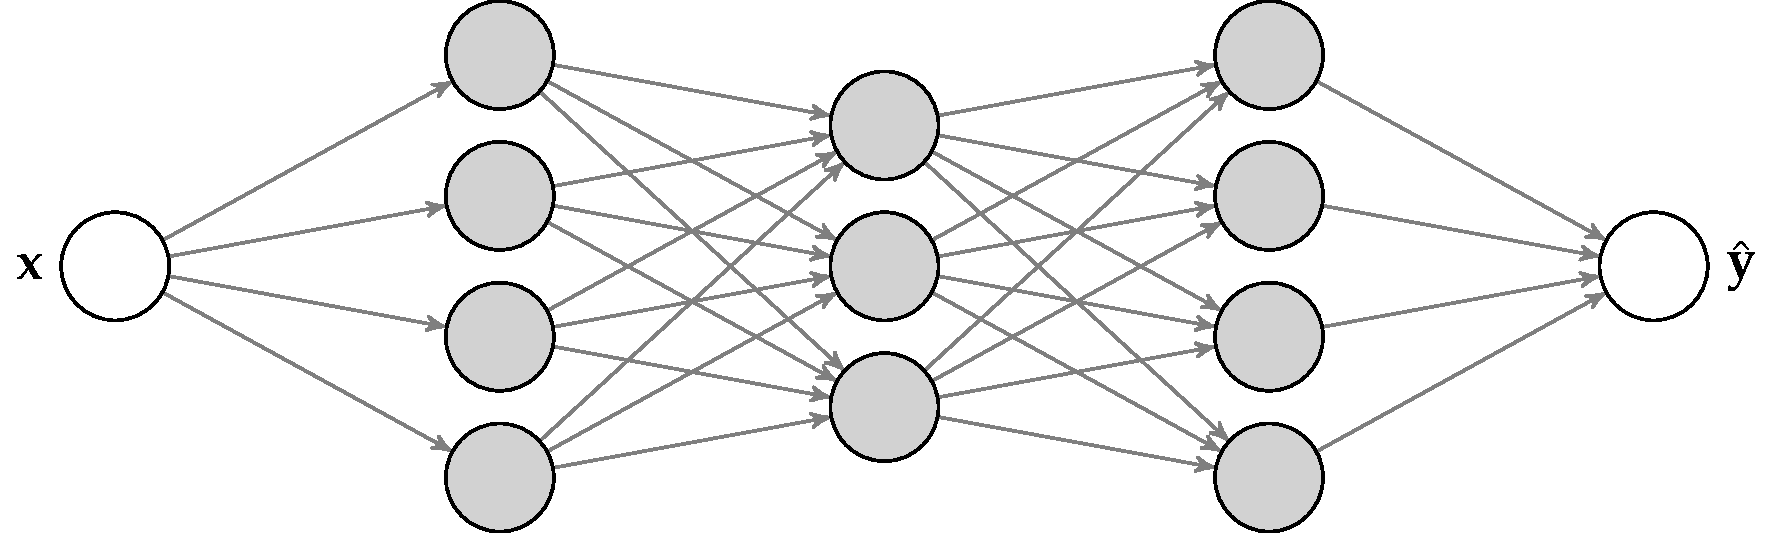
\includegraphics[width=0.85\textwidth]{diagrams/background/nn.pdf}
    \caption{Neural network surrogate model approximating $\hat{\mathbf{y}} = f_\theta(\mathbf{x})$.}
    \label{fig:ann}
\end{figure}

Neural networks are primarily used for two different tasks, namely classification and regression.
In multi-class classification (with $K$ classes), the objective of a gradient-based optimization method is to minimize the \textit{cross-entropy loss}:
\begin{equation}
    \mathcal{L}_{\text{CE}}(y, \hat{y}; \theta) = -\frac{1}{n}\sum_{i=1}^n\sum_{k=1}^K y^{(k)}_i \log \hat{y}^{(k)}_i
\end{equation}
where $y$ is the one-hot encoded true class label and $\hat{y}$ is the predicted probability distribution over the $K$ classes for $n$ batches.
The predicted probabilities are obtained by applying a \textit{softmax} function to the vector of logits $z = [z_1, \dots, z_K]$ output by the neural network:
\begin{equation}
    \hat{y}^{(k)} = \frac{\exp z_k}{\sum_{j=1}^K \exp z_j}
\end{equation}
For single-class classification, e.g., in cases where we want to predict a failure ($y = 1$) or success ($y=0$), the \textit{binary cross-entropy} loss is used instead:
\begin{equation}
    \mathcal{L}_{\text{BCE}}(y, \hat{y}; \theta) = -\frac{1}{n} \sum_{i=1}^n \Big( y_i \log \big(\sigma(\hat{y}_i)\big) + (1 - y_i) \log \big(1 - \sigma(\hat{y}_i)\big) \Big)
\end{equation}
where $\sigma(z) = 1 / (1 + \exp(-z))$ is the sigmoid function ensuring the prediction lies in $[0,1]$.

In regression tasks, the objective is to approximate a real-valued function for outputs $y \in \mathbb{R}^d$.
This is often done by minimizing the mean-squared error or mean-absolute error between the true output $y$ and prediction $\hat{y}$:
\begin{align}
    \mathcal{L}_\text{MSE}(y, \hat{y}; \theta) &= \frac{1}{n} \sum_{i=1}^n (y_i - \hat{y}_i)^2 \\
    \mathcal{L}_\text{MAE}(y, \hat{y}; \theta) &= \frac{1}{n} \sum_{i=1}^n |y_i - \hat{y}_i|
\end{align}

\Cref{ch:ivae} further details neural network surrogates and how they can be used as generative models to sample from the posterior belief given the current observations.



\section{Safety Validation}\label{sec:safety_validation}

To validate safety-critical systems, developers often perform \textit{safety validation} \cite{corso2021survey}.
Safety validation has three primary tasks shown in \cref{fig:safety_validation}.
Given a system under test $f(\mathbf{x})$, its design space $\mathbf{x} \in \mathcal{X}$, and a property specification $\psi$ \cite{donze2010robust}, where $f(\mathbf{x}) \not\in \psi$ indicates the system violated the specification, we get the following tasks:
\begin{enumerate}
    \item \textbf{Falsification:} The process of finding \textit{any} input $\mathbf{x}$ that results in a system failure \cite{donze2010breach}:
    \begin{equation}
        \mathbf{x} \quad \text{s.t.} \quad f(\mathbf{x}) \not\in \psi
    \end{equation}
    \item \textbf{Most-likely failure analysis:} Finding the failure with the maximum likelihood under the nominal distribution $p(\mathbf{x})$ \cite{lee2020adaptive}:
    \begin{equation}
        \argmax_{\mathbf{x} \in \mathcal{X}} p(\mathbf{x}) \quad \text{s.t.} \quad f(\mathbf{x}) \not\in \psi
    \end{equation}
    \item \textbf{Failure probability estimation:} Estimating the probability that a failure will occur under the nominal distribution $p(\mathbf{x})$ over the domain of the design space $\mathbf{x} \in \mathcal{X}$ \cite{gooley1999estimation}:
    \begin{equation}
        p_\text{fail} = \mathbf{E}_p \big[ \mathds{1}\{f(\mathbf{x}) \not\in \psi \} \big]
    \end{equation}
\end{enumerate}

If methods focus on failure probability estimation, then it is often the case that all three safety validation tasks can be achieved.
This is because when estimating the probability of failure, samples from the normalized distribution of failures are produced.
Thus, we achieve falsification by finding failures in the process of constructing the distribution and can easily compute the most-likely failure by maximizing the input likelihood across the nominal distribution.
Motivated to achieve all three safety validation tasks, the work in \cref{ch:bsv} develops an efficient approach to estimate probability of failure for black-box systems.
For a survey of existing black-box safety validation algorithms, including falsification and most-likely failure analysis, we refer to \textcite{corso2021survey}.


\begin{figure}[t]
    \centering
    \resizebox{\textwidth}{!}{%
          \tikzset{
    >={Latex[width=1.5mm,length=1.5mm]},
    end/.style = {circle, minimum width=2mm, minimum height=2mm},
    startstyle/.style = {rectangle, semithick, fill=\secondarycolor, draw=\primarycolor, minimum width=3mm, minimum height=3mm},
    successstyle/.style = {end,  fill=darkgreen},
    failurestyle/.style = {end, fill=darkred},
    sectionstyle/.style = {fill=none, draw=none, minimum height=2cm},
}

% https://tex.stackexchange.com/questions/33607/easy-curves-in-tikz

\begin{tikzpicture}

\node (falsification) [sectionstyle, label={[font=\color{\primarycolor}]above:\textsc{Falsification}}] {
\begin{tikzpicture}
    \node (start) [startstyle] {};

    \node (success) [successstyle, above right=3mm and 25mm of start, label={right:{\color{darkgreen}success}}] {};
    \node (failure) [failurestyle, below right=3mm and 25mm of start, label={right:{\color{darkred}failure}}] {};

    \draw [semithick,\primarycolor,->] plot [smooth] coordinates {(start.east) ($(start.east)+(3mm,0mm)$)  ($(start.east)+(6mm,-3mm)$) ($(start.east)+(13mm,1mm)$) ($(start.east)+(20mm,-10mm)$) (failure.south west)};
\end{tikzpicture}
};

\draw [gray] ($(falsification.east) + (0.4cm,-2)$) -- ($(falsification.east) + (0.4cm,2)$);

\node (mostlikely) [sectionstyle, right=of falsification, label={[align=center,font=\color{\primarycolor}]above:\textsc{Most-likely}\\\textsc{Failure Analysis}}] {
\begin{tikzpicture}
    \node (start) [startstyle] {};
    
    \node (success) [successstyle, above right=3mm and 25mm of start, label={right:{\color{darkgreen}success}}] {};   
    \node (failure) [failurestyle, below right=3mm and 25mm of start, label={right:{\color{darkred}failure}}] {};

    \draw [semithick,\primarycolor,->] plot [smooth] coordinates {(start.east) ($(start.east)+(10mm,1mm)$) (failure.north west)};
\end{tikzpicture}
};

\draw [gray] ($(mostlikely.east) + (0.4cm,-2)$) -- ($(mostlikely.east) + (0.4cm,2)$);

\node (failureprob) [sectionstyle, right=of mostlikely, label={[align=center,font=\color{\primarycolor}]above:\textsc{Failure Probability}\\\textsc{Estimation}}] {
\begin{tikzpicture}
    \node (start) [startstyle] {};
    
    \node (success) [successstyle, above right=3mm and 25mm of start, label={right:{\color{darkgreen}success}}] {};
    \node (failure) [failurestyle, below right=3mm and 25mm of start, label={right:{\color{darkred}failure}}] {};

    \draw [semithick,gray4,->] plot [smooth] coordinates {(start.east) ($(start.east)+(3mm,0mm)$)  ($(start.east)+(6mm,-3mm)$) ($(start.east)+(13mm,1mm)$) ($(start.east)+(20mm,-10mm)$) (failure.south west)};
    \draw [semithick,gray4,->] plot [smooth] coordinates {(start.east) ($(start.east)+(5mm,-2mm)$) ($(start.east)+(16mm,-12mm)$) (failure.south)};
    \draw [semithick,gray3,->] plot [smooth] coordinates {(start.east) ($(start.east)+(15mm,6mm)$) (failure.north)};
    \draw [semithick,gray2,->] plot [smooth] coordinates {(start.east) ($(start.east)+(5mm,-1mm)$) ($(start.east)+(15mm,-9mm)$) (failure.south west)};
    \draw [semithick,gray1,->] plot [smooth] coordinates {(start.east) ($(start.east)+(6mm,-1mm)$) ($(start.east)+(15mm,-6mm)$) (failure.west)};
    \draw [semithick,\primarycolor,->] plot [smooth] coordinates {(start.east) ($(start.east)+(10mm,1mm)$) (failure.north west)};
\end{tikzpicture}
};

\end{tikzpicture}

    }
    \caption{The three tasks of safety validation.}
    \label{fig:safety_validation}
\end{figure}


\paragraph{Black-box vs. white-box validation.}
In the case of \textit{black-box safety validation}, we treat the system $f$ as a ``black box'' and attempt to perform the three tasks described above.
The black-box assumption means that the only way to interact with the system is by passing inputs $\vec{x}$ and observing outputs $y = f(\vec{x})$.
This is in contrast to \textit{white-box validation} which requires information about the internals of the system to prove properties of safety \cite{schumann2001automated,fitting2012firstorder,clarke2018handbook}.
In choosing to perform black-box validation, we can apply methods to more general systems, particularly to systems with neural network components.
Although recent work has focused on verifying small neural networks \cite{katz2017reluplex,liu2021algorithms,sidrane2022overt}, scaling to large networks remains a challenge \cite{konig2024critically}.
\Cref{ch:bsv} investigates an approach that attempts to address this challenge.
